\documentclass{beamer}

\usetheme{Warsaw}
\usecolortheme{orchid}

\usepackage{algorithm,algorithmic}
\usepackage{amssymb}
\usepackage{amsthm}
\usepackage{pgfplots} 
\usepackage{graphicx}
\usepackage[utf8x]{inputenc}
\usepackage{tikz}
\usepackage{bbm}
\usepackage{subcaption}
\usepackage{mathtools}
\usepackage{lipsum}
\usepackage{color}
\usepackage{physics}
\usepackage{appendixnumberbeamer}

\DeclarePairedDelimiter{\ceil}{\lceil}{\rceil}
\newcommand{\eqtext}[1]{\ensuremath{\stackrel{#1}{=}}}
\newcommand{\leqtext}[1]{\ensuremath{\stackrel{#1}{\leq}}}
\newcommand{\diffL}{\mathcal{L}}
\newcommand{\N}{\mathbb{N}}
\newcommand{\R}{\mathbb{R}}
\newcommand{\E}{\mathbb{E}}
\newcommand{\epl}{\varepsilon}
\newcommand{\defeq}{\coloneqq}
\newcommand{\uDarcy}{\color{red}{u}}
\newcommand{\sksum}{\textstyle\sum}
\newcommand{\MSE}{\operatorname{MSE}}
\newcommand{\Var}{\operatorname{Var}}
\newcommand{\OO}{\mathcal{O}}
\newcommand{\Hell}{d_{\mathrm{Hell}}}
\newtheorem{proposition}[theorem]{Proposition}
\newtheorem{problemTh}{Problem}
\newtheorem{assumption}{Assumption}
\renewcommand{\phi}{\varphi}
\definecolor{mygray}{gray}{0.8}
\newcommand{\eqdef}{\eqqcolon}

% Add numbers and take out navigation symbols
\setbeamertemplate{footline}[frame number]
\beamertemplatenavigationsymbolsempty

\title{Probabilistic solvers for ODE's \\ and Bayesian inference of parametrized models}
\subtitle{Master Project - Master in CSE}
\author{Giacomo Garegnani \\ Supervisor: Prof. Assyr Abdulle \\ Expert: Dr. Kostas Zygalakis}
\institute{EPFL}
\date{02/02/2017}

\begin{document}

\frame{\titlepage}

%%%%%%%%%%%%%%%%%%%%%%%%%%%%%%%%%%%%%%%%%%%%%%%%%%%%%%%%%%%%
%%%%%%%%%%%%%%%%%%%%%%%%%%%%%%%%%%%% OUTLINE %%%%%%%%%%%%%%%
%%%%%%%%%%%%%%%%%%%%%%%%%%%%%%%%%%%%%%%%%%%%%%%%%%%%%%%%%%%%
\begin{frame}
	\frametitle{Outline of the presentation}
	\begin{enumerate}
		\item Introduction on Bayesian inference and MCMC
		\item Probabilistic solvers for ODE's
		\item Bayesian inference inverse problems with differential equations
	\end{enumerate}
\end{frame}

%%%%%%%%%%%%%%%%%%%%%%%%%%%%%%%%%%%%%%%%%%%%%%%%%%%%%%%%%%%%
%%%%%%%%%%%%%%%%%%%%%%%%%%%%%%%%%%%% PART ONE %%%%%%%%%%%%%%
%%%%%%%%%%%%%%%%%%%%%%%%%%%%%%%%%%%%%%%%%%%%%%%%%%%%%%%%%%%%

\begin{frame}
	\frametitle{Bayesian inference and MCMC}
	\framesubtitle{Bayes' formula}
	
	Consider $\Omega$ event space, $\mathcal{A}$  $\sigma$-algebra, $P$ probability measure and $(\Omega, \mathcal{A}, P)$. Given $A$, $B$ in $\Omega$, Bayes' formula reads 
	\begin{equation*}
		P(A\mid B) = \frac{P(B\mid A)P(A)}{P(B)} \propto P(B\mid A)P(A).
	\end{equation*}
	Normalization constant $P(B)$ can be replaced as
	\begin{equation*}
		P(A\mid B) = \frac{P(B\mid A)P(A)}{\int_{\Omega}P(B\mid A)P(A)},
	\end{equation*}
	as $P(A\mid B)$ is a probability distribution.
\end{frame}

\begin{frame}
	\frametitle{Bayesian inference and MCMC}
	\framesubtitle{Bayesian inference}
	
	\underline{Problem.} Consider two events $A$, $B$ in $\Omega$ and the probability space $(\Omega, \mathcal{A}, P)$. We want to infer the probability distribution of $A$ given $B$ as
	\begin{equation*}
		\underbrace{\pi(A\mid B)}_{\text{posterior}} \propto \overbrace{\mathcal{Q}(A)}^{\text{prior}} \underbrace{\mathcal{L}(B \mid A)}_{\text{likelihood}}
	\end{equation*}
	In models parametrized by a parameter $\theta$, we deduce the distribution of $\theta$ through observations $\mathcal{Y}_n = \{y_1, y_2, \ldots, y_n\}$ as
	\begin{equation*}
		\pi(\theta\mid\mathcal{Y}_n) \propto \mathcal{Q}(\theta) \mathcal{L}(\mathcal{Y}_n \mid \theta).
	\end{equation*}
\end{frame}

\begin{frame}
	\frametitle{Bayesian inference and MCMC}
	\framesubtitle{MCMC - motivation}
	
	\underline{Goal.} Approximate the expectation under the distribution $\pi(\theta \mid \mathcal{Y})$ of a functional of the parameter $\theta \in \R^{N_p}$ with a Monte Carlo sum, i.e.,
	\begin{equation*}\label{eq:MonteCarlo}
			 \E^\pi\left[g(\theta)\right] = \int_{\R^{N_p}} g(\theta)\pi(\dd\theta\mid\mathcal{Y})  \approx \frac{1}{N}\sum_{k = 1}^{N} g(\theta^{(k)}),
	\end{equation*}
	where $\theta^{(k)}$ are realizations of $\theta$. \\[0.5cm]
	\underline{Problem.} Generate samples $\theta^{(k)}$, with $k = 1, \ldots, N$ so that the approximation above holds
	$\rightsquigarrow$ MCMC \cite[e.g.]{Gil05} \\[0.5cm]
	\underline{Idea.} Generate samples $\theta^{(k)}$ from a Markov chain with kernel $P$ until the chain reaches its \textit{stationary distribution}. Different choices of the Markov kernel lead to different MCMC algorithms.	
\end{frame}

\begin{frame}
	\frametitle{Bayesian inference and MCMC}
	\framesubtitle{Metropolis-Hastings}
	\begin{algorithm}[H]	
		\begin{algorithmic}
			\STATE Given $\theta^{(0)} \in \R^{N_p}, N \in \N_0$, $q(x, y)\colon \int q(x,y)\dd y = 1$;
			\FOR{$i = 0, \ldots, N$}
			\STATE Draw $\vartheta$ from $q(\theta^{(i)}, \cdot)$;
			\STATE Compute \textit{acceptance probability} $\alpha(\theta^{(i)}, \vartheta)$ as $$\alpha(\theta^{(i)}, \vartheta) = \min\left\{\frac{\pi(\vartheta)q(\vartheta, \theta^{(i)})}{\pi(\theta^{(i)})q(\theta^{(i)}, \vartheta)}, 1\right\};$$
			\STATE Draw $u$ from $\mathcal{U}(0, 1)$;
			\IF{$\alpha > u$}
			\STATE Accept $\vartheta$, set $\theta^{(i+1)} = \vartheta$; 
			\ELSE
			\STATE set $\theta^{(i+1)} = \theta^{(i)}$;
			\ENDIF
			\ENDFOR
		\end{algorithmic}
		\caption{Metropolis-Hastings.}
	\end{algorithm}
\end{frame}

\begin{frame}
	\frametitle{Bayesian inference and MCMC}
	\framesubtitle{Metropolis-Hastings - Observations}
	
	\underline{Remark.} If the proposal distribution is symmetric, i.e., $q(x,y) = q(y,x)$, then 
	\begin{equation*}
		\alpha(\theta^{(i)}, \vartheta) = \min\left\{\frac{\pi(\vartheta)q(\vartheta, \theta^{(i)})}{\pi(\theta^{(i)})q(\theta^{(i)}, \vartheta)}, 1\right\} = \min\left\{\frac{\pi(\vartheta)}{\pi(\theta^{(i)})}, 1\right\}.
	\end{equation*}
	For example, Gaussian proposal \cite{KaS05}
	\begin{equation*}
		q(x, y) \propto \exp(-\frac{1}{2}(x - y)^T\Sigma^{-1}(x - y)).
	\end{equation*}
	\underline{Problems.} 
	\begin{enumerate}
		\item How to choose an efficient proposal distribution?
		\item How to modify MH if it is not possible to evaluate the posterior distribution?
	\end{enumerate}
\end{frame}

\begin{frame}
	\frametitle{Bayesian inference and MCMC}
	\framesubtitle{Robust adaptive Metropolis (RAM) \cite{Vih12}}
	
	\underline{Problem.} Bad proposal distribution $q(x,y) \implies$ inefficient algorithms. Measure efficiency with \textit{acceptance ratio}. \\[0.5cm]
	\underline{Idea.} Adapt $q(x,y)$ to obtain a chosen acceptance ratio $\alpha^*$. Choose $q(x,y)$ Gaussian, the new guess $\vartheta$ is 
	\begin{equation*}
		\vartheta = \theta^{(n)} + S_n z_n, \quad Z_n \sim \mathcal{N}(0, I),
	\end{equation*}
	where $S_n \in \R^{N_p\times N_p}$ is lower triangular definite positive. Then, 
	\begin{equation*}
		S_{n+1}S_{n+1}^T = S_n\left(I + \eta_n\left(\alpha(\theta^{(n)}, \vartheta) - \alpha^*\right)\frac{z_nz_n^T}{z_n^Tz_n}\right)S_n^T,
	\end{equation*}
	where $\eta_n \xrightarrow{n\to\infty} 0$.
	
\end{frame}

\begin{frame}
	\frametitle{Bayesian inference and MCMC}
	\framesubtitle{Robust adaptive Metropolis \cite{Vih12}, numerical experiment}
	
	Two-dimensional distribution $\pi$ with density \cite{KaS05}
	\begin{equation*}
		\pi(X) \propto \exp(-10(X_1^2 - X_2)^2 - (X_1 - 0.25)^4),
	\end{equation*}
	Setting of the experiment. Given $\sigma = \{0.01, 0.5, 2.0\}$, compare
	\begin{itemize}
		\item standard MH with Gaussian proposal with covariance $\sigma I$,
		\item RAM with $S_0 = \sigma I$ and $\alpha^* = 0.4$.
	\end{itemize}
	Draw $N = 5000$ samples and compute obtained acceptance ratio as
	\begin{equation*}
		\bar \alpha = \frac{\text{n. of accepted samples } \vartheta}{N}
	\end{equation*}
\end{frame}


\begin{frame}
	\frametitle{Bayesian inference and MCMC}
	\framesubtitle{Robust adaptive Metropolis \cite{Vih12}, numerical experiment}
	\begin{figure}[t]
		\centering
		\begin{subfigure}{0.32\linewidth}
			\centering
			\tiny{$\bar \alpha = 0.96$}
			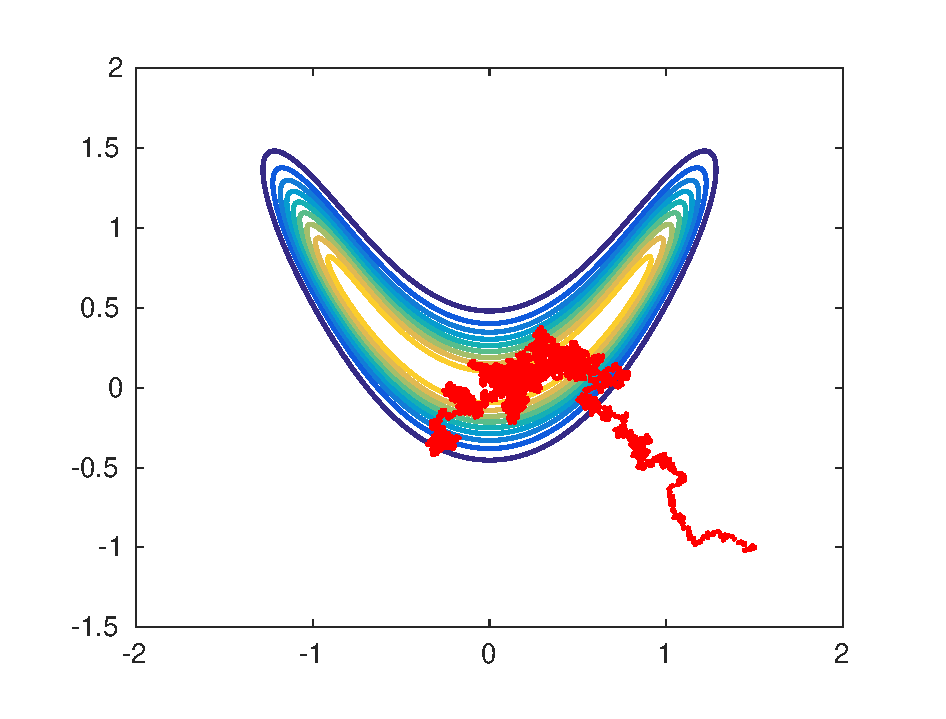
\includegraphics[width=1\linewidth]{../plots/MHvsRAM/MH_small}
		\end{subfigure}
		\begin{subfigure}{0.32\linewidth}
			\centering
			\tiny{$\bar \alpha = 0.35$}
			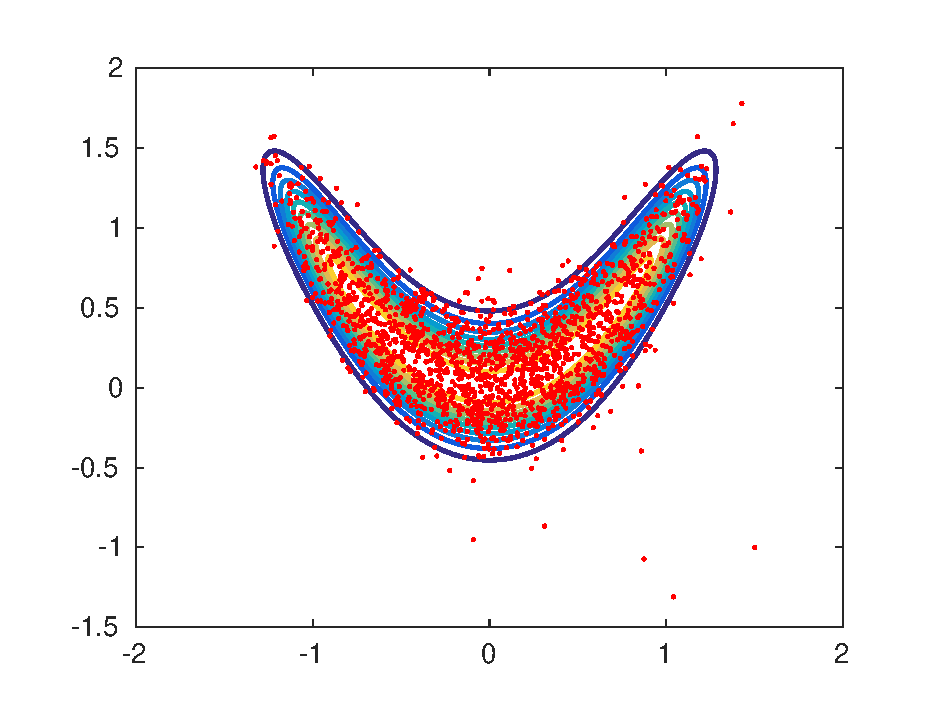
\includegraphics[width=1\linewidth]{../plots/MHvsRAM/MH_medium}
		\end{subfigure}
		\begin{subfigure}{0.32\linewidth}
			\centering
			\tiny{$\bar \alpha = 0.06$}
			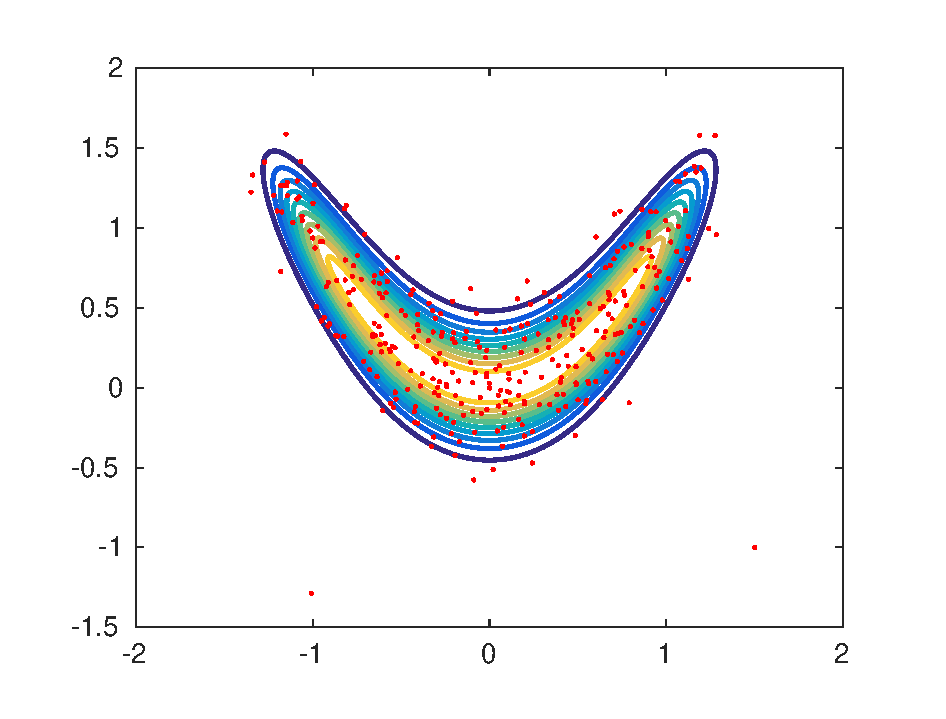
\includegraphics[width=1\linewidth]{../plots/MHvsRAM/MH_big}
		\end{subfigure}
		
		\begin{subfigure}{0.32\linewidth}
			\centering
			\tiny{$\bar \alpha = 0.43$}
			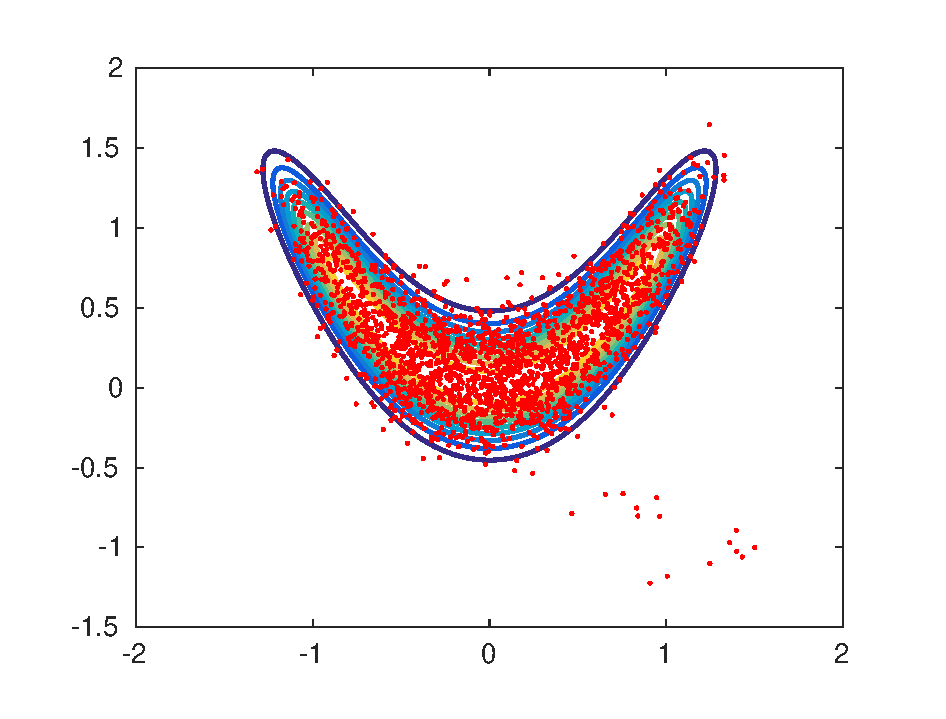
\includegraphics[width=1\linewidth]{../plots/MHvsRAM/RAM_small}
		\end{subfigure}
		\begin{subfigure}{0.32\linewidth}
			\centering
			\tiny{$\bar \alpha = 0.40$}
			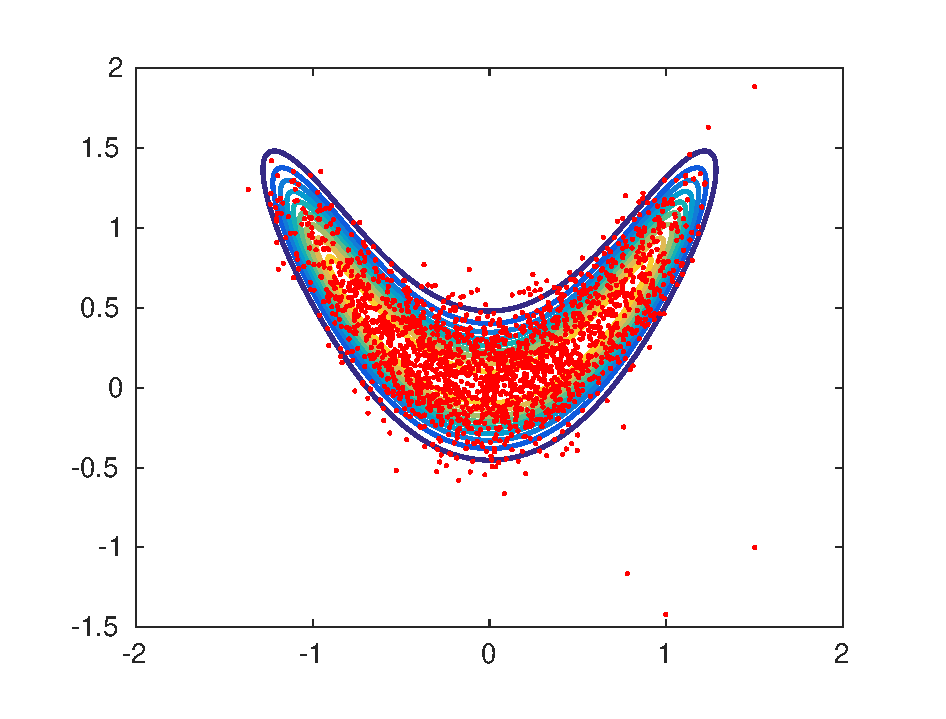
\includegraphics[width=1\linewidth]{../plots/MHvsRAM/RAM_medium}
		\end{subfigure}
		\begin{subfigure}{0.32\linewidth}
			\centering
			\tiny{$\bar \alpha = 0.38$}
			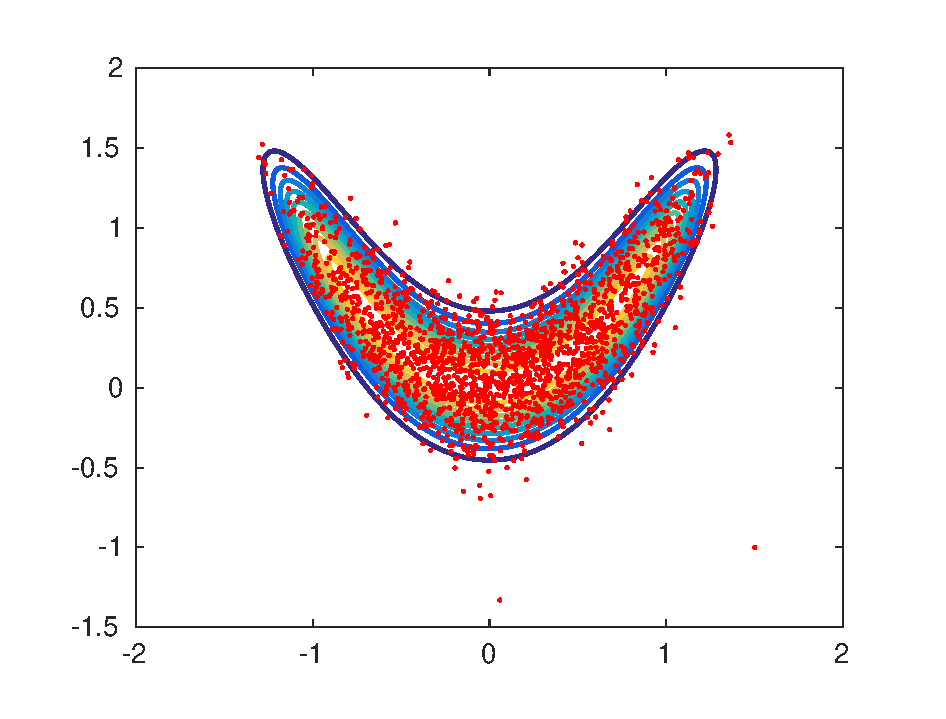
\includegraphics[width=1\linewidth]{../plots/MHvsRAM/RAM_big}
		\end{subfigure}
	\end{figure}
	Samples produced by MH and RAM for the distribution with standard MH (first row) and RAM (second row).
\end{frame}

\begin{frame}
	\frametitle{Bayesian inference and MCMC}
	\framesubtitle{Pseudo-marginal MCMC \cite{ADH10, DPD15, MLR16}}
	
	\underline{Problem.} Impossible to evaluate $\pi(\theta)$ (no closed form available). \\[0.5cm]
	\underline{Idea.} Find evaluable $\pi(\theta, \xi)$ that admits $\pi(\theta)$ as marginal distribution, then compute
	\begin{equation*}
		\hat \pi_M(\theta) = \frac{1}{M} \sum_{i = 1}^{M} \pi(\theta, \xi^{(i)}),
	\end{equation*}
	with $\xi^{(i)}$, $i = 1, \ldots, M$ realizations of $\xi$. Use $\hat \pi_M$ for $\alpha(\theta^{(i)}, \vartheta)$. \\[0.5cm]
	\underline{Remark.} The rest of MH is unchanged.	
\end{frame}

%%%%%%%%%%%%%%%%%%%%%%%%%%%%%%%%%%%%%%%%%%%%%%%%%%%%%%%%%%%%
%%%%%%%%%%%%%%%%%%%%%%%%%%%%%%%%%%%% PART TWO %%%%%%%%%%%%%%
%%%%%%%%%%%%%%%%%%%%%%%%%%%%%%%%%%%%%%%%%%%%%%%%%%%%%%%%%%%%

\begin{frame}
	\frametitle{Outline of the presentation}
	\begin{enumerate}
		\item \color{mygray} Introduction on Bayesian inference and MCMC
		\item \color{black} Probabilistic solvers for ODE's
		\item Bayesian inference inverse problems with differential equations
	\end{enumerate}
\end{frame}

\begin{frame}
	\frametitle{Probabilistic solvers for ODE's}
	\framesubtitle{Method presentation \cite{CGS16}}
	
	\underline{Problem.} Given $f\colon\R^d\to\R^d$ and the autonomous ODE 
	\begin{equation*}
		u'(t) = f(u), \quad	u(0) = u_0, 
	\end{equation*}
	build a probabilistic numerical solution. There exists flow map $\Phi_t(y)$ such that
	\begin{equation*}
		u(t) = \Phi_t(u_0).
	\end{equation*}
	\underline{Idea.} Given $h > 0$, the flow map of a Runge-Kutta method $\Psi_h(y)$ is
	\begin{equation*}
		u_{k+1} = \Psi_h(u_k), \quad k = 0, 1, \ldots,
	\end{equation*}
	consider $\xi_k(h)$ i.i.d. random variables in $\R^d$ and compute
	\begin{equation*}
		U_{k+1} = \underbrace{\Psi_h(U_k)}_{\text{deterministic}} + \overbrace{\xi_k(h)}^{\text{random}}, \quad k = 0, 1, \ldots,
	\end{equation*}
	
\end{frame}

\begin{frame}
	\frametitle{Probabilistic solvers for ODE's}
	\framesubtitle{Method motivation}
	
	Consider chaotic differential equation, e.g., Lorenz system
	\begin{equation*}\label{eq:Lorenz}
	\begin{aligned}
		x' &= \sigma(y - x), \quad &&x(0) = -10,\\
		y' &= x(\rho - z) - y, \quad &&y(0) = -1,\\
		z' &= xy - \beta z, \quad &&z(0) = 40,\\
		\sigma &= 10, \quad \rho = 28, \quad \beta = \frac{8}{3}.
	\end{aligned}
	\end{equation*}
	Small perturbation $\implies$ uncontrollable deviation of the solution. \\
	Deterministic solvers not reliable for any time step $h > 0$. \\
	$\rightsquigarrow$ Family of $M$ probabilistic numerical solutions.
\end{frame}

\begin{frame}
	\frametitle{Probabilistic solvers for ODE's}
	\framesubtitle{Method motivation}
	
	\begin{figure}[t]
		\centering
		\begin{subfigure}{1\linewidth}
			\resizebox{1.0\linewidth}{!}{% This file was created by matlab2tikz.
%
%The latest EFupdates can be retrieved from
%  http://www.mathworks.com/matlabcentral/fileexchange/22022-matlab2tikz-matlab2tikz
%where you can also make suggestions and rate matlab2tikz.
%
\begin{tikzpicture}

\begin{axis}[%
width=10.783in,
height=3in,
at={(1.809in,1.132in)},
scale only axis,
xmin=0,
xmax=20,
ymin=-20,
ymax=20,
axis background/.style={fill=white},
axis x line*=bottom,
axis y line*=left,
ylabel = {$x$},
ylabel style = {font=\LARGE},
ticklabel style={font=\LARGE},legend style={font=\LARGE},title style={font=\LARGE}
]
\addplot [color=white!65!black,solid,line width=0.0pt,forget plot]
  table[row sep=crcr]{%
0	-10\\
0.05	-5.53726\\
0.1	-2.11573\\
0.15	0.00290185\\
0.2	1.243\\
0.25	2.07127\\
0.3	2.83212\\
0.35	3.76911\\
0.4	5.07637\\
0.45	6.91238\\
0.5	9.31371\\
0.55	11.9319\\
0.6	13.7307\\
0.65	13.4256\\
0.7	10.939\\
0.75	7.6592\\
0.8	4.90597\\
0.85	3.11777\\
0.9	2.17349\\
0.95	1.82389\\
1	1.88526\\
1.05	2.28038\\
1.1	3.03009\\
1.15	4.23953\\
1.2	6.07584\\
1.25	8.67801\\
1.3	11.8547\\
1.35	14.5188\\
1.4	14.7739\\
1.45	11.9736\\
1.5	7.86494\\
1.55	4.36306\\
1.6	2.07385\\
1.65	0.779623\\
1.7	0.0912073\\
1.75	-0.297369\\
1.8	-0.580875\\
1.85	-0.882299\\
1.9	-1.29757\\
1.95	-1.93266\\
2	-2.9359\\
2.05	-4.5252\\
2.1	-6.98077\\
2.15	-10.4717\\
2.2	-14.4101\\
2.25	-16.5548\\
2.3	-14.5195\\
2.35	-9.50439\\
2.4	-4.63478\\
2.45	-1.3018\\
2.5	0.670719\\
2.55	1.86014\\
2.6	2.75657\\
2.65	3.69883\\
2.7	4.92602\\
2.75	6.61407\\
2.8	8.82711\\
2.85	11.3163\\
2.9	13.24\\
2.95	13.3948\\
3	11.4189\\
3.05	8.38538\\
3.1	5.62454\\
3.15	3.73239\\
3.2	2.69504\\
3.25	2.30201\\
3.3	2.3757\\
3.35	2.83754\\
3.4	3.7082\\
3.45	5.08908\\
3.5	7.11599\\
3.55	9.80975\\
3.6	12.7058\\
3.65	14.4678\\
3.7	13.6221\\
3.75	10.445\\
3.8	6.76369\\
3.85	3.91259\\
3.9	2.14911\\
3.95	1.21714\\
4	0.803274\\
4.05	0.69067\\
4.1	0.768019\\
4.15	1.00336\\
4.2	1.42436\\
4.25	2.11464\\
4.3	3.22491\\
4.35	4.98752\\
4.4	7.68515\\
4.45	11.398\\
4.5	15.2112\\
4.55	16.5316\\
4.6	13.5273\\
4.65	8.26251\\
4.7	3.67817\\
4.75	0.691149\\
4.8	-1.05683\\
4.85	-2.14931\\
4.9	-3.0425\\
4.95	-4.04801\\
5	-5.38819\\
5.05	-7.21605\\
5.1	-9.53107\\
5.15	-11.9392\\
5.2	-13.4441\\
5.25	-12.9653\\
5.3	-10.5781\\
5.35	-7.55759\\
5.4	-5.04928\\
5.45	-3.43443\\
5.5	-2.61484\\
5.55	-2.38232\\
5.6	-2.59001\\
5.65	-3.19243\\
5.7	-4.23811\\
5.75	-5.84355\\
5.8	-8.11841\\
5.85	-10.9437\\
5.9	-13.5427\\
5.95	-14.3797\\
6	-12.512\\
6.05	-8.99153\\
6.1	-5.60438\\
6.15	-3.22329\\
6.2	-1.84405\\
6.25	-1.168\\
6.3	-0.922954\\
6.35	-0.944707\\
6.4	-1.16741\\
6.45	-1.60093\\
6.5	-2.32066\\
6.55	-3.47236\\
6.6	-5.27881\\
6.65	-7.99266\\
6.7	-11.6186\\
6.75	-15.1482\\
6.8	-16.1093\\
6.85	-13.0512\\
6.9	-8.04999\\
6.95	-3.7558\\
7	-0.964672\\
7.05	0.661168\\
7.1	1.6603\\
7.15	2.45503\\
7.2	3.33751\\
7.25	4.52774\\
7.3	6.21094\\
7.35	8.49411\\
7.4	11.1964\\
7.45	13.4827\\
7.5	13.9456\\
7.55	11.9529\\
7.6	8.62465\\
7.65	5.53215\\
7.7	3.39303\\
7.75	2.18408\\
7.8	1.64408\\
7.85	1.5455\\
7.9	1.76617\\
7.95	2.28522\\
8	3.16859\\
8.05	4.56004\\
8.1	6.65537\\
8.15	9.57181\\
8.2	12.9293\\
8.25	15.2284\\
8.3	14.4834\\
8.35	10.8197\\
8.4	6.52229\\
8.45	3.23864\\
8.5	1.21334\\
8.55	0.079742\\
8.6	-0.573965\\
8.65	-1.04549\\
8.7	-1.53263\\
8.75	-2.18721\\
8.8	-3.16518\\
8.85	-4.66141\\
8.9	-6.90371\\
8.95	-10.0081\\
9	-13.4896\\
9.05	-15.6056\\
9.1	-14.3343\\
9.15	-10.2309\\
9.2	-5.82348\\
9.25	-2.61182\\
9.3	-0.67399\\
9.35	0.425366\\
9.4	1.11428\\
9.45	1.69623\\
9.5	2.38271\\
9.55	3.35239\\
9.6	4.79528\\
9.65	6.91185\\
9.7	9.78543\\
9.75	12.9739\\
9.8	14.991\\
9.85	14.0749\\
9.9	10.5205\\
9.95	6.46498\\
10	3.38577\\
10.05	1.49565\\
10.1	0.459756\\
10.15	-0.0954721\\
10.2	-0.434648\\
10.25	-0.722625\\
10.3	-1.06993\\
10.35	-1.57545\\
10.4	-2.3618\\
10.45	-3.60662\\
10.5	-5.56081\\
10.55	-8.49019\\
10.6	-12.3266\\
10.65	-15.7773\\
10.7	-16.1102\\
10.75	-12.3404\\
10.8	-7.1129\\
10.85	-2.93651\\
10.9	-0.31362\\
10.95	1.21571\\
11	2.208\\
11.05	3.07664\\
11.1	4.10573\\
11.15	5.50569\\
11.2	7.4227\\
11.25	9.83304\\
11.3	12.2724\\
11.35	13.6438\\
11.4	12.8819\\
11.45	10.2513\\
11.5	7.15116\\
11.55	4.68047\\
11.6	3.13508\\
11.65	2.3704\\
11.7	2.16553\\
11.75	2.37483\\
11.8	2.95689\\
11.85	3.96472\\
11.9	5.52407\\
11.95	7.77132\\
12	10.6512\\
12.05	13.471\\
12.1	14.6523\\
12.15	12.9865\\
12.2	9.38101\\
12.25	5.77205\\
12.3	3.18823\\
12.35	1.66432\\
12.4	0.880569\\
12.45	0.531508\\
12.5	0.420811\\
12.55	0.448859\\
12.6	0.581706\\
12.65	0.830212\\
12.7	1.24405\\
12.75	1.91956\\
12.8	3.01967\\
12.85	4.79786\\
12.9	7.57857\\
12.95	11.503\\
13	15.637\\
13.05	17.0761\\
13.1	13.721\\
13.15	7.98438\\
13.2	3.11738\\
13.25	0.00161994\\
13.3	-1.8233\\
13.35	-3.00137\\
13.4	-4.01439\\
13.45	-5.17603\\
13.5	-6.67828\\
13.55	-8.57814\\
13.6	-10.6746\\
13.65	-12.3429\\
13.7	-12.6923\\
13.75	-11.3434\\
13.8	-8.95226\\
13.85	-6.56761\\
13.9	-4.81796\\
13.95	-3.82614\\
14	-3.48516\\
14.05	-3.67171\\
14.1	-4.33014\\
14.15	-5.47858\\
14.2	-7.16508\\
14.25	-9.34787\\
14.3	-11.6563\\
14.35	-13.1817\\
14.4	-12.892\\
14.45	-10.7481\\
14.5	-7.87786\\
14.55	-5.40917\\
14.6	-3.78028\\
14.65	-2.94179\\
14.7	-2.70896\\
14.75	-2.9432\\
14.8	-3.60121\\
14.85	-4.72932\\
14.9	-6.42876\\
14.95	-8.7562\\
15	-11.4688\\
15.05	-13.6461\\
15.1	-13.8692\\
15.15	-11.6651\\
15.2	-8.28816\\
15.25	-5.26511\\
15.3	-3.22074\\
15.35	-2.0866\\
15.4	-1.59522\\
15.45	-1.5269\\
15.5	-1.76883\\
15.55	-2.30787\\
15.6	-3.2163\\
15.65	-4.64345\\
15.7	-6.78803\\
15.75	-9.75705\\
15.8	-13.1236\\
15.85	-15.3114\\
15.9	-14.3625\\
15.95	-10.5724\\
16	-6.28191\\
16.05	-3.06027\\
16.1	-1.09055\\
16.15	0.0115172\\
16.2	0.656289\\
16.25	1.13725\\
16.3	1.65086\\
16.35	2.35162\\
16.4	3.40176\\
16.45	5.00267\\
16.5	7.37575\\
16.55	10.5772\\
16.6	13.9494\\
16.65	15.5856\\
16.7	13.7471\\
16.75	9.47772\\
16.8	5.2559\\
16.85	2.29574\\
16.9	0.542254\\
16.95	-0.449782\\
17	-1.0828\\
17.05	-1.63601\\
17.1	-2.3058\\
17.15	-3.26376\\
17.2	-4.69923\\
17.25	-6.81934\\
17.3	-9.7241\\
17.35	-12.9914\\
17.4	-15.114\\
17.45	-14.2355\\
17.5	-10.6084\\
17.55	-6.44619\\
17.6	-3.28716\\
17.65	-1.34686\\
17.7	-0.272965\\
17.75	0.324939\\
17.8	0.725654\\
17.85	1.10893\\
17.9	1.60527\\
17.95	2.34309\\
18	3.48683\\
18.05	5.25993\\
18.1	7.90716\\
18.15	11.4366\\
18.2	14.9062\\
18.25	15.9725\\
18.3	13.1499\\
18.35	8.31084\\
18.4	4.05833\\
18.45	1.25921\\
18.5	-0.37155\\
18.55	-1.35173\\
18.6	-2.09636\\
18.65	-2.8929\\
18.7	-3.95823\\
18.75	-5.48594\\
18.8	-7.6333\\
18.85	-10.3654\\
18.9	-13.0763\\
18.95	-14.3536\\
19	-13.0096\\
19.05	-9.71104\\
19.1	-6.23841\\
19.15	-3.67075\\
19.2	-2.13312\\
19.25	-1.35837\\
19.3	-1.0651\\
19.35	-1.07359\\
19.4	-1.30767\\
19.45	-1.77357\\
19.5	-2.54844\\
19.55	-3.78263\\
19.6	-5.69924\\
19.65	-8.52345\\
19.7	-12.1488\\
19.75	-15.3572\\
19.8	-15.7027\\
19.85	-12.2846\\
19.9	-7.41775\\
19.95	-3.43692\\
20	-0.902631\\
};
\addplot [color=white!65!black,solid,line width=0.0pt,forget plot]
  table[row sep=crcr]{%
0	-10\\
0.05	-5.53725\\
0.1	-2.11573\\
0.15	0.00290251\\
0.2	1.243\\
0.25	2.07128\\
0.3	2.83212\\
0.35	3.76912\\
0.4	5.07637\\
0.45	6.91239\\
0.5	9.31372\\
0.55	11.932\\
0.6	13.7307\\
0.65	13.4256\\
0.7	10.939\\
0.75	7.65919\\
0.8	4.90597\\
0.85	3.11777\\
0.9	2.17349\\
0.95	1.82389\\
1	1.88527\\
1.05	2.28039\\
1.1	3.0301\\
1.15	4.23955\\
1.2	6.07587\\
1.25	8.67804\\
1.3	11.8548\\
1.35	14.5188\\
1.4	14.7739\\
1.45	11.9735\\
1.5	7.8649\\
1.55	4.36303\\
1.6	2.07384\\
1.65	0.779622\\
1.7	0.0912115\\
1.75	-0.297362\\
1.8	-0.580863\\
1.85	-0.88228\\
1.9	-1.29754\\
1.95	-1.93262\\
2	-2.93584\\
2.05	-4.52512\\
2.1	-6.98066\\
2.15	-10.4716\\
2.2	-14.41\\
2.25	-16.5548\\
2.3	-14.5197\\
2.35	-9.50459\\
2.4	-4.63492\\
2.45	-1.30186\\
2.5	0.670691\\
2.55	1.86013\\
2.6	2.75657\\
2.65	3.69883\\
2.7	4.92602\\
2.75	6.61406\\
2.8	8.82708\\
2.85	11.3162\\
2.9	13.24\\
2.95	13.3948\\
3	11.4189\\
3.05	8.38542\\
3.1	5.62459\\
3.15	3.73244\\
3.2	2.69509\\
3.25	2.30206\\
3.3	2.37575\\
3.35	2.8376\\
3.4	3.70827\\
3.45	5.08918\\
3.5	7.1161\\
3.55	9.80986\\
3.6	12.7059\\
3.65	14.4678\\
3.7	13.622\\
3.75	10.4449\\
3.8	6.76359\\
3.85	3.91255\\
3.9	2.14912\\
3.95	1.21718\\
4	0.803345\\
4.05	0.690772\\
4.1	0.768159\\
4.15	1.00356\\
4.2	1.42464\\
4.25	2.11507\\
4.3	3.22555\\
4.35	4.98848\\
4.4	7.68651\\
4.45	11.3996\\
4.5	15.2123\\
4.55	16.531\\
4.6	13.5253\\
4.65	8.26045\\
4.7	3.6768\\
4.75	0.690443\\
4.8	-1.05712\\
4.85	-2.14942\\
4.9	-3.04255\\
4.95	-4.04809\\
5	-5.38836\\
5.05	-7.21637\\
5.1	-9.53155\\
5.15	-11.9397\\
5.2	-13.4444\\
5.25	-12.9652\\
5.3	-10.5776\\
5.35	-7.55692\\
5.4	-5.04865\\
5.45	-3.4339\\
5.5	-2.6144\\
5.55	-2.38192\\
5.6	-2.58962\\
5.65	-3.192\\
5.7	-4.23762\\
5.75	-5.84298\\
5.8	-8.1178\\
5.85	-10.9432\\
5.9	-13.5426\\
5.95	-14.3802\\
6	-12.5128\\
6.05	-8.9922\\
6.1	-5.60465\\
6.15	-3.22321\\
6.2	-1.84372\\
6.25	-1.16747\\
6.3	-0.922241\\
6.35	-0.943753\\
6.4	-1.1661\\
6.45	-1.59907\\
6.5	-2.31796\\
6.55	-3.46837\\
6.6	-5.27297\\
6.65	-7.98463\\
6.7	-11.6094\\
6.75	-15.1426\\
6.8	-16.1132\\
6.85	-13.0627\\
6.9	-8.06139\\
6.95	-3.76317\\
7	-0.968296\\
7.05	0.659893\\
7.1	1.66021\\
7.15	2.4554\\
7.2	3.33791\\
7.25	4.5279\\
7.3	6.21055\\
7.35	8.49288\\
7.4	11.1942\\
7.45	13.4801\\
7.5	13.9442\\
7.55	11.9537\\
7.6	8.62715\\
7.65	5.53525\\
7.7	3.39612\\
7.75	2.18705\\
7.8	1.64709\\
7.85	1.54886\\
7.9	1.77025\\
7.95	2.29051\\
8	3.17574\\
8.05	4.56981\\
8.1	6.66835\\
8.15	9.58717\\
8.2	12.9422\\
8.25	15.2293\\
8.3	14.4686\\
8.35	10.799\\
8.4	6.50657\\
8.45	3.23062\\
8.5	1.21133\\
8.55	0.0815477\\
8.6	-0.569711\\
8.65	-1.03928\\
8.7	-1.52427\\
8.75	-2.17593\\
8.8	-3.14972\\
8.85	-4.64015\\
8.9	-6.87553\\
8.95	-9.97542\\
9	-13.4643\\
9.05	-15.6086\\
9.1	-14.3701\\
9.15	-10.2747\\
9.2	-5.85396\\
9.25	-2.62571\\
9.3	-0.675796\\
9.35	0.430987\\
9.4	1.12463\\
9.45	1.71041\\
9.5	2.40112\\
9.55	3.37629\\
9.6	4.82624\\
9.65	6.95038\\
9.7	9.82704\\
9.75	13.0027\\
9.8	14.983\\
9.85	14.0276\\
9.9	10.4649\\
9.95	6.42807\\
10	3.37213\\
10.05	1.4996\\
10.1	0.475486\\
10.15	-0.0708016\\
10.2	-0.400819\\
10.25	-0.676677\\
10.3	-1.00594\\
10.35	-1.48354\\
10.4	-2.22647\\
10.45	-3.40486\\
10.5	-5.26365\\
10.55	-8.08119\\
10.6	-11.871\\
10.65	-15.5308\\
10.7	-16.3649\\
10.75	-12.9431\\
10.8	-7.66571\\
10.85	-3.27708\\
10.9	-0.473901\\
10.95	1.16233\\
11	2.20459\\
11.05	3.0881\\
11.1	4.11041\\
11.15	5.48704\\
11.2	7.36522\\
11.25	9.72699\\
11.3	12.1337\\
11.35	13.5353\\
11.4	12.8774\\
11.45	10.3565\\
11.5	7.31102\\
11.55	4.84587\\
11.6	3.28763\\
11.65	2.5125\\
11.7	2.30819\\
11.75	2.53179\\
11.8	3.14309\\
11.85	4.19553\\
11.9	5.81081\\
11.95	8.10511\\
12	10.965\\
12.05	13.606\\
12.1	14.458\\
12.15	12.5523\\
12.2	8.97113\\
12.25	5.53912\\
12.3	3.13424\\
12.35	1.74113\\
12.4	1.05041\\
12.45	0.782337\\
12.5	0.766151\\
12.55	0.92781\\
12.6	1.2648\\
12.65	1.83349\\
12.7	2.75268\\
12.75	4.21764\\
12.8	6.49628\\
12.85	9.79881\\
12.9	13.7393\\
12.95	16.3908\\
13	15.1352\\
13.05	10.4486\\
13.1	5.42709\\
13.15	1.83233\\
13.2	-0.327073\\
13.25	-1.60432\\
13.3	-2.5115\\
13.35	-3.40876\\
13.4	-4.54826\\
13.45	-6.12078\\
13.5	-8.23288\\
13.55	-10.7425\\
13.6	-12.9566\\
13.65	-13.6468\\
13.7	-12.1016\\
13.75	-9.12796\\
13.8	-6.16658\\
13.85	-4.02175\\
13.9	-2.77857\\
13.95	-2.23469\\
14	-2.18681\\
14.05	-2.52582\\
14.1	-3.24531\\
14.15	-4.42729\\
14.2	-6.21306\\
14.25	-8.70819\\
14.3	-11.6987\\
14.35	-14.1648\\
14.4	-14.4118\\
14.45	-11.8632\\
14.5	-8.05315\\
14.55	-4.73998\\
14.6	-2.54509\\
14.65	-1.31431\\
14.7	-0.70769\\
14.75	-0.454031\\
14.8	-0.392897\\
14.85	-0.44933\\
14.9	-0.604492\\
14.95	-0.879361\\
15	-1.33291\\
15.05	-2.07332\\
15.1	-3.28061\\
15.15	-5.22906\\
15.2	-8.24586\\
15.25	-12.3657\\
15.3	-16.2881\\
15.35	-16.8414\\
15.4	-12.6786\\
15.45	-6.87682\\
15.5	-2.32031\\
15.55	0.50531\\
15.6	2.16566\\
15.65	3.28839\\
15.7	4.32057\\
15.75	5.54797\\
15.8	7.13464\\
15.85	9.08787\\
15.9	11.1166\\
15.95	12.5087\\
16	12.4386\\
16.05	10.7811\\
16.1	8.35467\\
16.15	6.12988\\
16.2	4.59076\\
16.25	3.7841\\
16.3	3.59234\\
16.35	3.90951\\
16.4	4.70082\\
16.45	5.99498\\
16.5	7.82252\\
16.55	10.0642\\
16.6	12.1972\\
16.65	13.2153\\
16.7	12.3123\\
16.75	9.86501\\
16.8	7.09318\\
16.85	4.9094\\
16.9	3.56484\\
16.95	2.94957\\
17	2.89127\\
17.05	3.28519\\
17.1	4.12079\\
17.15	5.46529\\
17.2	7.40801\\
17.25	9.90719\\
17.3	12.4688\\
17.35	13.9046\\
17.4	13.0527\\
17.45	10.2284\\
17.5	6.96251\\
17.55	4.40119\\
17.6	2.81307\\
17.65	2.016\\
17.7	1.7631\\
17.75	1.89145\\
17.8	2.34474\\
17.85	3.16144\\
17.9	4.46159\\
17.95	6.42057\\
18	9.15767\\
18.05	12.3817\\
18.1	14.8153\\
18.15	14.5542\\
18.2	11.3529\\
18.25	7.20593\\
18.3	3.86584\\
18.35	1.7484\\
18.4	0.567296\\
18.45	-0.0678897\\
18.5	-0.448643\\
18.55	-0.759777\\
18.6	-1.12378\\
18.65	-1.64625\\
18.7	-2.45375\\
18.75	-3.72593\\
18.8	-5.71171\\
18.85	-8.66233\\
18.9	-12.4657\\
18.95	-15.7701\\
19	-15.9075\\
19.05	-12.0906\\
19.1	-6.96835\\
19.15	-2.9171\\
19.2	-0.381898\\
19.25	1.09323\\
19.3	2.04781\\
19.35	2.8817\\
19.4	3.87165\\
19.45	5.22848\\
19.5	7.11288\\
19.55	9.54224\\
19.6	12.1185\\
19.65	13.7593\\
19.7	13.2439\\
19.75	10.6496\\
19.8	7.40542\\
19.85	4.7507\\
19.9	3.05616\\
19.95	2.18131\\
20	1.88292\\
};
\addplot [color=white!65!black,solid,line width=0.0pt,forget plot]
  table[row sep=crcr]{%
0	-10\\
0.05	-5.53726\\
0.1	-2.11573\\
0.15	0.00290269\\
0.2	1.243\\
0.25	2.07127\\
0.3	2.83212\\
0.35	3.76911\\
0.4	5.07637\\
0.45	6.91238\\
0.5	9.31371\\
0.55	11.932\\
0.6	13.7307\\
0.65	13.4256\\
0.7	10.939\\
0.75	7.6592\\
0.8	4.90597\\
0.85	3.11777\\
0.9	2.17349\\
0.95	1.82389\\
1	1.88527\\
1.05	2.28039\\
1.1	3.03009\\
1.15	4.23954\\
1.2	6.07585\\
1.25	8.67802\\
1.3	11.8547\\
1.35	14.5188\\
1.4	14.7739\\
1.45	11.9735\\
1.5	7.86492\\
1.55	4.36305\\
1.6	2.07385\\
1.65	0.779623\\
1.7	0.0912114\\
1.75	-0.297364\\
1.8	-0.580865\\
1.85	-0.882282\\
1.9	-1.29754\\
1.95	-1.93263\\
2	-2.93585\\
2.05	-4.52513\\
2.1	-6.98067\\
2.15	-10.4716\\
2.2	-14.41\\
2.25	-16.5548\\
2.3	-14.5197\\
2.35	-9.50456\\
2.4	-4.6349\\
2.45	-1.30186\\
2.5	0.670692\\
2.55	1.86013\\
2.6	2.75657\\
2.65	3.69883\\
2.7	4.92602\\
2.75	6.61406\\
2.8	8.82709\\
2.85	11.3162\\
2.9	13.24\\
2.95	13.3948\\
3	11.4189\\
3.05	8.38542\\
3.1	5.62459\\
3.15	3.73244\\
3.2	2.69508\\
3.25	2.30206\\
3.3	2.37575\\
3.35	2.8376\\
3.4	3.70826\\
3.45	5.08917\\
3.5	7.11608\\
3.55	9.80984\\
3.6	12.7059\\
3.65	14.4678\\
3.7	13.622\\
3.75	10.4449\\
3.8	6.76361\\
3.85	3.91256\\
3.9	2.14912\\
3.95	1.21718\\
4	0.80334\\
4.05	0.690764\\
4.1	0.768144\\
4.15	1.00354\\
4.2	1.42462\\
4.25	2.11503\\
4.3	3.22549\\
4.35	4.9884\\
4.4	7.6864\\
4.45	11.3995\\
4.5	15.2122\\
4.55	16.5311\\
4.6	13.5255\\
4.65	8.26062\\
4.7	3.67692\\
4.75	0.690505\\
4.8	-1.05709\\
4.85	-2.1494\\
4.9	-3.04253\\
4.95	-4.04808\\
5	-5.38834\\
5.05	-7.21633\\
5.1	-9.5315\\
5.15	-11.9397\\
5.2	-13.4444\\
5.25	-12.9653\\
5.3	-10.5777\\
5.35	-7.55698\\
5.4	-5.0487\\
5.45	-3.43394\\
5.5	-2.61443\\
5.55	-2.38194\\
5.6	-2.58963\\
5.65	-3.19202\\
5.7	-4.23763\\
5.75	-5.84299\\
5.8	-8.11781\\
5.85	-10.9432\\
5.9	-13.5426\\
5.95	-14.3802\\
6	-12.5128\\
6.05	-8.9922\\
6.1	-5.60466\\
6.15	-3.22323\\
6.2	-1.84374\\
6.25	-1.1675\\
6.3	-0.922269\\
6.35	-0.943787\\
6.4	-1.16615\\
6.45	-1.59914\\
6.5	-2.31805\\
6.55	-3.46851\\
6.6	-5.27317\\
6.65	-7.9849\\
6.7	-11.6098\\
6.75	-15.1428\\
6.8	-16.1131\\
6.85	-13.0623\\
6.9	-8.06101\\
6.95	-3.76293\\
7	-0.968176\\
7.05	0.659931\\
7.1	1.6602\\
7.15	2.45538\\
7.2	3.33788\\
7.25	4.52787\\
7.3	6.21055\\
7.35	8.4929\\
7.4	11.1943\\
7.45	13.4802\\
7.5	13.9442\\
7.55	11.9537\\
7.6	8.62709\\
7.65	5.53516\\
7.7	3.39601\\
7.75	2.18694\\
7.8	1.64697\\
7.85	1.54872\\
7.9	1.77008\\
7.95	2.29028\\
8	3.17543\\
8.05	4.56939\\
8.1	6.66778\\
8.15	9.58649\\
8.2	12.9416\\
8.25	15.2292\\
8.3	14.4692\\
8.35	10.7999\\
8.4	6.50727\\
8.45	3.23098\\
8.5	1.21144\\
8.55	0.0814906\\
8.6	-0.569875\\
8.65	-1.03952\\
8.7	-1.5246\\
8.75	-2.17637\\
8.8	-3.15032\\
8.85	-4.64098\\
8.9	-6.87663\\
8.95	-9.97669\\
9	-13.4653\\
9.05	-15.6085\\
9.1	-14.3687\\
9.15	-10.273\\
9.2	-5.85278\\
9.25	-2.62519\\
9.3	-0.675746\\
9.35	0.430747\\
9.4	1.1242\\
9.45	1.70983\\
9.5	2.40037\\
9.55	3.37531\\
9.6	4.82496\\
9.65	6.94878\\
9.7	9.82532\\
9.75	13.0015\\
9.8	14.9833\\
9.85	14.0295\\
9.9	10.4672\\
9.95	6.42961\\
10	3.37272\\
10.05	1.49946\\
10.1	0.474862\\
10.15	-0.0717895\\
10.2	-0.402184\\
10.25	-0.67853\\
10.3	-1.00852\\
10.35	-1.48726\\
10.4	-2.23194\\
10.45	-3.41304\\
10.5	-5.27573\\
10.55	-8.09797\\
10.6	-11.8901\\
10.65	-15.542\\
10.7	-16.3555\\
10.75	-12.9182\\
10.8	-7.64223\\
10.85	-3.26236\\
10.9	-0.46685\\
10.95	1.16478\\
11	2.20489\\
11.05	3.08775\\
11.1	4.11034\\
11.15	5.48797\\
11.2	7.36779\\
11.25	9.73157\\
11.3	12.1396\\
11.35	13.5399\\
11.4	12.8775\\
11.45	10.352\\
11.5	7.30422\\
11.55	4.8389\\
11.6	3.28128\\
11.65	2.50667\\
11.7	2.30242\\
11.75	2.52553\\
11.8	3.13575\\
11.85	4.18654\\
11.9	5.79981\\
11.95	8.09257\\
12	10.9537\\
12.05	13.602\\
12.1	14.4663\\
12.15	12.5688\\
12.2	8.98594\\
12.25	5.54703\\
12.3	3.13546\\
12.35	1.73749\\
12.4	1.04324\\
12.45	0.771983\\
12.5	0.751965\\
12.55	0.908141\\
12.6	1.23675\\
12.65	1.79234\\
12.7	2.69116\\
12.75	4.12533\\
12.8	6.36177\\
12.85	9.62285\\
12.9	13.573\\
12.95	16.3606\\
13	15.3064\\
13.05	10.6954\\
13.1	5.61777\\
13.15	1.94022\\
13.2	-0.278484\\
13.25	-1.58757\\
13.3	-2.5075\\
13.35	-3.4058\\
13.4	-4.53852\\
13.45	-6.09778\\
13.5	-8.19148\\
13.55	-10.6839\\
13.6	-12.8987\\
13.65	-13.6237\\
13.7	-12.1322\\
13.75	-9.1946\\
13.8	-6.24066\\
13.85	-4.08777\\
13.9	-2.8344\\
13.95	-2.28421\\
14	-2.2354\\
14.05	-2.57878\\
14.1	-3.30772\\
14.15	-4.50371\\
14.2	-6.30551\\
14.25	-8.80946\\
14.3	-11.7795\\
14.35	-14.1719\\
14.4	-14.3188\\
14.45	-11.7259\\
14.5	-7.94824\\
14.55	-4.69484\\
14.6	-2.55082\\
14.65	-1.35571\\
14.7	-0.775975\\
14.75	-0.548857\\
14.8	-0.521968\\
14.85	-0.629063\\
14.9	-0.863001\\
14.95	-1.26265\\
15	-1.91534\\
15.05	-2.97276\\
15.1	-4.67214\\
15.15	-7.32079\\
15.2	-11.0772\\
15.25	-15.1615\\
15.3	-16.9284\\
15.35	-14.0989\\
15.4	-8.60332\\
15.45	-3.70203\\
15.5	-0.488649\\
15.55	1.39683\\
15.6	2.58078\\
15.65	3.55294\\
15.7	4.64073\\
15.75	6.0602\\
15.8	7.92225\\
15.85	10.1288\\
15.9	12.1619\\
15.95	13.0599\\
16	12.1083\\
16.05	9.72096\\
16.1	7.05983\\
16.15	4.97591\\
16.2	3.70341\\
16.25	3.14219\\
16.3	3.13519\\
16.35	3.59024\\
16.4	4.50421\\
16.45	5.94165\\
16.5	7.96397\\
16.55	10.4483\\
16.6	12.7685\\
16.65	13.7121\\
16.7	12.4139\\
16.75	9.51247\\
16.8	6.47112\\
16.85	4.202\\
16.9	2.85246\\
16.95	2.23127\\
17	2.12464\\
17.05	2.4088\\
17.1	3.06385\\
17.15	4.16093\\
17.2	5.83801\\
17.25	8.22381\\
17.3	11.1949\\
17.35	13.8923\\
17.4	14.6297\\
17.45	12.4719\\
17.5	8.6923\\
17.55	5.19099\\
17.6	2.78911\\
17.65	1.40853\\
17.7	0.70781\\
17.75	0.392895\\
17.8	0.281316\\
17.85	0.280346\\
17.9	0.35449\\
17.95	0.504208\\
18	0.757942\\
18.05	1.17556\\
18.1	1.86249\\
18.15	2.9947\\
18.2	4.84761\\
18.25	7.7765\\
18.3	11.9269\\
18.35	16.2054\\
18.4	17.3559\\
18.45	13.401\\
18.5	7.31513\\
18.55	2.39937\\
18.6	-0.672279\\
18.65	-2.47218\\
18.7	-3.67109\\
18.75	-4.74489\\
18.8	-5.985\\
18.85	-7.53562\\
18.9	-9.36048\\
18.95	-11.1306\\
19	-12.1865\\
19.05	-11.8963\\
19.1	-10.2946\\
19.15	-8.13118\\
19.2	-6.20208\\
19.25	-4.89668\\
19.3	-4.2589\\
19.35	-4.20322\\
19.4	-4.65356\\
19.45	-5.58675\\
19.5	-7.0098\\
19.55	-8.87119\\
19.6	-10.8887\\
19.65	-12.3871\\
19.7	-12.518\\
19.75	-11.0346\\
19.8	-8.66107\\
19.85	-6.38858\\
19.9	-4.76578\\
19.95	-3.87992\\
20	-3.62383\\
};
\addplot [color=white!65!black,solid,line width=0.0pt,forget plot]
  table[row sep=crcr]{%
0	-10\\
0.05	-5.53726\\
0.1	-2.11573\\
0.15	0.00290209\\
0.2	1.243\\
0.25	2.07127\\
0.3	2.83212\\
0.35	3.76911\\
0.4	5.07636\\
0.45	6.91238\\
0.5	9.31371\\
0.55	11.9319\\
0.6	13.7307\\
0.65	13.4256\\
0.7	10.939\\
0.75	7.6592\\
0.8	4.90597\\
0.85	3.11777\\
0.9	2.17348\\
0.95	1.82389\\
1	1.88526\\
1.05	2.28037\\
1.1	3.03008\\
1.15	4.23952\\
1.2	6.07583\\
1.25	8.678\\
1.3	11.8547\\
1.35	14.5188\\
1.4	14.7739\\
1.45	11.9736\\
1.5	7.86496\\
1.55	4.36307\\
1.6	2.07385\\
1.65	0.779619\\
1.7	0.0911986\\
1.75	-0.297382\\
1.8	-0.58089\\
1.85	-0.882318\\
1.9	-1.2976\\
1.95	-1.93271\\
2	-2.93596\\
2.05	-4.5253\\
2.1	-6.98091\\
2.15	-10.4719\\
2.2	-14.4103\\
2.25	-16.5548\\
2.3	-14.5194\\
2.35	-9.50416\\
2.4	-4.63462\\
2.45	-1.30171\\
2.5	0.670756\\
2.55	1.86015\\
2.6	2.75657\\
2.65	3.69883\\
2.7	4.92603\\
2.75	6.61409\\
2.8	8.82715\\
2.85	11.3163\\
2.9	13.2401\\
2.95	13.3948\\
3	11.4189\\
3.05	8.38532\\
3.1	5.62448\\
3.15	3.73234\\
3.2	2.69499\\
3.25	2.30197\\
3.3	2.37566\\
3.35	2.8375\\
3.4	3.70815\\
3.45	5.08902\\
3.5	7.11592\\
3.55	9.80968\\
3.6	12.7058\\
3.65	14.4679\\
3.7	13.6222\\
3.75	10.4451\\
3.8	6.76375\\
3.85	3.91261\\
3.9	2.14909\\
3.95	1.2171\\
4	0.803215\\
4.05	0.690593\\
4.1	0.767911\\
4.15	1.00321\\
4.2	1.42414\\
4.25	2.11431\\
4.3	3.22441\\
4.35	4.98677\\
4.4	7.68409\\
4.45	11.3967\\
4.5	15.2103\\
4.55	16.532\\
4.6	13.5289\\
4.65	8.26413\\
4.7	3.67924\\
4.75	0.691701\\
4.8	-1.05659\\
4.85	-2.14923\\
4.9	-3.04246\\
4.95	-4.04795\\
5	-5.38804\\
5.05	-7.21578\\
5.1	-9.53066\\
5.15	-11.9387\\
5.2	-13.4438\\
5.25	-12.9654\\
5.3	-10.5785\\
5.35	-7.55813\\
5.4	-5.04979\\
5.45	-3.43485\\
5.5	-2.61518\\
5.55	-2.38262\\
5.6	-2.59031\\
5.65	-3.19276\\
5.7	-4.23848\\
5.75	-5.84398\\
5.8	-8.11886\\
5.85	-10.9441\\
5.9	-13.5427\\
5.95	-14.3793\\
6	-12.5113\\
6.05	-8.99105\\
6.1	-5.60419\\
6.15	-3.22337\\
6.2	-1.84432\\
6.25	-1.1684\\
6.3	-0.923504\\
6.35	-0.945444\\
6.4	-1.16842\\
6.45	-1.60236\\
6.5	-2.32274\\
6.55	-3.47543\\
6.6	-5.28329\\
6.65	-7.99882\\
6.7	-11.6256\\
6.75	-15.1525\\
6.8	-16.1063\\
6.85	-13.0423\\
6.9	-8.04125\\
6.95	-3.75015\\
7	-0.961903\\
7.05	0.662136\\
7.1	1.66036\\
7.15	2.45474\\
7.2	3.33718\\
7.25	4.52761\\
7.3	6.21122\\
7.35	8.49503\\
7.4	11.1981\\
7.45	13.4847\\
7.5	13.9467\\
7.55	11.9523\\
7.6	8.62278\\
7.65	5.5298\\
7.7	3.39068\\
7.75	2.18182\\
7.8	1.64176\\
7.85	1.54292\\
7.9	1.76303\\
7.95	2.28114\\
8	3.1631\\
8.05	4.55252\\
8.1	6.64536\\
8.15	9.55996\\
8.2	12.9194\\
8.25	15.2277\\
8.3	14.4949\\
8.35	10.8356\\
8.4	6.53446\\
8.45	3.24487\\
8.5	1.21493\\
8.55	0.0783758\\
8.6	-0.577218\\
8.65	-1.05025\\
8.7	-1.53905\\
8.75	-2.19585\\
8.8	-3.17701\\
8.85	-4.67765\\
8.9	-6.92521\\
8.95	-10.033\\
9	-13.5087\\
9.05	-15.6029\\
9.1	-14.307\\
9.15	-10.1978\\
9.2	-5.80045\\
9.25	-2.60141\\
9.3	-0.672743\\
9.35	0.42097\\
9.4	1.10628\\
9.45	1.68528\\
9.5	2.36847\\
9.55	3.33388\\
9.6	4.77122\\
9.65	6.88182\\
9.7	9.75279\\
9.75	12.9509\\
9.8	14.9966\\
9.85	14.1116\\
9.9	10.5641\\
9.95	6.49428\\
10	3.39688\\
10.05	1.49299\\
10.1	0.447878\\
10.15	-0.114282\\
10.2	-0.460481\\
10.25	-0.757695\\
10.3	-1.11872\\
10.35	-1.6454\\
10.4	-2.46457\\
10.45	-3.75926\\
10.5	-5.78396\\
10.55	-8.79222\\
10.6	-12.6491\\
10.65	-15.9229\\
10.7	-15.8895\\
10.75	-11.8997\\
10.8	-6.72967\\
10.85	-2.70788\\
10.9	-0.210036\\
10.95	1.24655\\
11	2.20513\\
11.05	3.06372\\
11.1	4.09732\\
11.15	5.51314\\
11.2	7.45724\\
11.25	9.90275\\
11.3	12.3679\\
11.35	13.7222\\
11.4	12.89\\
11.45	10.1826\\
11.5	7.04204\\
11.55	4.56447\\
11.6	3.02511\\
11.65	2.26491\\
11.7	2.0566\\
11.75	2.25198\\
11.8	2.808\\
11.85	3.77626\\
11.9	5.28407\\
11.95	7.48166\\
12	10.3596\\
12.05	13.3099\\
12.1	14.7754\\
12.15	13.3535\\
12.2	9.7618\\
12.25	6.01019\\
12.3	3.26882\\
12.35	1.62792\\
12.4	0.76343\\
12.45	0.348868\\
12.5	0.166561\\
12.55	0.0963942\\
12.6	0.0803052\\
12.65	0.094421\\
12.7	0.13317\\
12.75	0.202427\\
12.8	0.31859\\
12.85	0.51228\\
12.9	0.837082\\
12.95	1.38547\\
13	2.31538\\
13.05	3.88813\\
13.1	6.4925\\
13.15	10.5014\\
13.2	15.4435\\
13.25	18.341\\
13.3	15.5333\\
13.35	8.94106\\
13.4	3.002\\
13.45	-0.829\\
13.5	-3.05126\\
13.55	-4.44098\\
13.6	-5.55665\\
13.65	-6.7155\\
13.7	-8.03865\\
13.75	-9.45358\\
13.8	-10.6699\\
13.85	-11.2476\\
13.9	-10.874\\
13.95	-9.66775\\
14	-8.12229\\
14.05	-6.74583\\
14.1	-5.82224\\
14.15	-5.42556\\
14.2	-5.53132\\
14.25	-6.09721\\
14.3	-7.08205\\
14.35	-8.40714\\
14.4	-9.87057\\
14.45	-11.0703\\
14.5	-11.4896\\
14.55	-10.8445\\
14.6	-9.38196\\
14.65	-7.69829\\
14.7	-6.30648\\
14.75	-5.44142\\
14.8	-5.13275\\
14.85	-5.3356\\
14.9	-6.00619\\
14.95	-7.10962\\
15	-8.56711\\
15.05	-10.1515\\
15.1	-11.398\\
15.15	-11.725\\
15.2	-10.8668\\
15.25	-9.18177\\
15.3	-7.36002\\
15.35	-5.92537\\
15.4	-5.07687\\
15.45	-4.80979\\
15.5	-5.06322\\
15.55	-5.79395\\
15.6	-6.97825\\
15.65	-8.55087\\
15.7	-10.2825\\
15.75	-11.6624\\
15.8	-12.0218\\
15.85	-11.0498\\
15.9	-9.16961\\
15.95	-7.1729\\
16	-5.62784\\
16.05	-4.72304\\
16.1	-4.42833\\
16.15	-4.66547\\
16.2	-5.38858\\
16.25	-6.58829\\
16.3	-8.2325\\
16.35	-10.1344\\
16.4	-11.7868\\
16.45	-12.413\\
16.5	-11.5274\\
16.55	-9.50684\\
16.6	-7.26214\\
16.65	-5.48442\\
16.7	-4.40382\\
16.75	-3.97752\\
16.8	-4.10198\\
16.85	-4.71587\\
16.9	-5.81731\\
16.95	-7.42179\\
17	-9.44614\\
17.05	-11.5033\\
17.1	-12.7737\\
17.15	-12.4213\\
17.2	-10.48\\
17.25	-7.91923\\
17.3	-5.70409\\
17.35	-4.23823\\
17.4	-3.50931\\
17.45	-3.37801\\
17.5	-3.73862\\
17.55	-4.56577\\
17.6	-5.90164\\
17.65	-7.79244\\
17.7	-10.1294\\
17.75	-12.3702\\
17.8	-13.4344\\
17.85	-12.4502\\
17.9	-9.84376\\
17.95	-6.93613\\
18	-4.67576\\
18.05	-3.29389\\
18.1	-2.65182\\
18.15	-2.55715\\
18.2	-2.89335\\
18.25	-3.6437\\
18.3	-4.87796\\
18.35	-6.71249\\
18.4	-9.19217\\
18.45	-11.9907\\
18.5	-14.0195\\
18.55	-13.8104\\
18.6	-11.1785\\
18.65	-7.64723\\
18.7	-4.68797\\
18.75	-2.76761\\
18.8	-1.73011\\
18.85	-1.28507\\
18.9	-1.21461\\
18.95	-1.4097\\
19	-1.85473\\
19.05	-2.61234\\
19.1	-3.8205\\
19.15	-5.6876\\
19.2	-8.42266\\
19.25	-11.9243\\
19.3	-15.0646\\
19.35	-15.5485\\
19.4	-12.4089\\
19.45	-7.72917\\
19.5	-3.80261\\
19.55	-1.26844\\
19.6	0.19225\\
19.65	1.06168\\
19.7	1.71494\\
19.75	2.41014\\
19.8	3.34578\\
19.85	4.71222\\
19.9	6.70114\\
19.95	9.40358\\
20	12.4654\\
};
\addplot [color=white!65!black,solid,line width=0.0pt,forget plot]
  table[row sep=crcr]{%
0	-10\\
0.05	-5.53726\\
0.1	-2.11573\\
0.15	0.00290342\\
0.2	1.243\\
0.25	2.07128\\
0.3	2.83212\\
0.35	3.76912\\
0.4	5.07637\\
0.45	6.91239\\
0.5	9.31372\\
0.55	11.932\\
0.6	13.7307\\
0.65	13.4256\\
0.7	10.939\\
0.75	7.65919\\
0.8	4.90596\\
0.85	3.11777\\
0.9	2.17348\\
0.95	1.82389\\
1	1.88527\\
1.05	2.28039\\
1.1	3.03009\\
1.15	4.23955\\
1.2	6.07586\\
1.25	8.67804\\
1.3	11.8548\\
1.35	14.5188\\
1.4	14.7739\\
1.45	11.9735\\
1.5	7.86491\\
1.55	4.36303\\
1.6	2.07384\\
1.65	0.779616\\
1.7	0.091205\\
1.75	-0.29737\\
1.8	-0.580874\\
1.85	-0.882296\\
1.9	-1.29756\\
1.95	-1.93266\\
2	-2.93589\\
2.05	-4.52519\\
2.1	-6.98076\\
2.15	-10.4717\\
2.2	-14.4101\\
2.25	-16.5548\\
2.3	-14.5196\\
2.35	-9.50441\\
2.4	-4.63479\\
2.45	-1.30179\\
2.5	0.670724\\
2.55	1.86015\\
2.6	2.75658\\
2.65	3.69885\\
2.7	4.92604\\
2.75	6.61409\\
2.8	8.82713\\
2.85	11.3163\\
2.9	13.24\\
2.95	13.3947\\
3	11.4189\\
3.05	8.38536\\
3.1	5.62454\\
3.15	3.7324\\
3.2	2.69505\\
3.25	2.30203\\
3.3	2.37573\\
3.35	2.83758\\
3.4	3.70824\\
3.45	5.08915\\
3.5	7.11607\\
3.55	9.80983\\
3.6	12.7059\\
3.65	14.4678\\
3.7	13.622\\
3.75	10.4449\\
3.8	6.76361\\
3.85	3.91255\\
3.9	2.1491\\
3.95	1.21715\\
4	0.803299\\
4.05	0.690711\\
4.1	0.768074\\
4.15	1.00344\\
4.2	1.42448\\
4.25	2.11482\\
4.3	3.22517\\
4.35	4.98792\\
4.4	7.68572\\
4.45	11.3987\\
4.5	15.2117\\
4.55	16.5314\\
4.6	13.5265\\
4.65	8.26165\\
4.7	3.67759\\
4.75	0.690844\\
4.8	-1.05696\\
4.85	-2.14937\\
4.9	-3.04253\\
4.95	-4.04806\\
5	-5.38828\\
5.05	-7.2162\\
5.1	-9.53128\\
5.15	-11.9394\\
5.2	-13.4442\\
5.25	-12.9653\\
5.3	-10.5779\\
5.35	-7.5573\\
5.4	-5.04902\\
5.45	-3.43422\\
5.5	-2.61467\\
5.55	-2.38216\\
5.6	-2.58986\\
5.65	-3.19228\\
5.7	-4.23793\\
5.75	-5.84335\\
5.8	-8.1182\\
5.85	-10.9436\\
5.9	-13.5427\\
5.95	-14.3799\\
6	-12.5123\\
6.05	-8.99175\\
6.1	-5.60445\\
6.15	-3.22324\\
6.2	-1.84391\\
6.25	-1.16779\\
6.3	-0.922676\\
6.35	-0.944338\\
6.4	-1.16691\\
6.45	-1.60021\\
6.5	-2.31961\\
6.55	-3.47083\\
6.6	-5.27656\\
6.65	-7.98957\\
6.7	-11.6151\\
6.75	-15.146\\
6.8	-16.1108\\
6.85	-13.0556\\
6.9	-8.05437\\
6.95	-3.75863\\
7	-0.966058\\
7.05	0.660688\\
7.1	1.66028\\
7.15	2.45519\\
7.2	3.33768\\
7.25	4.52782\\
7.3	6.21082\\
7.35	8.49367\\
7.4	11.1956\\
7.45	13.4817\\
7.5	13.945\\
7.55	11.9532\\
7.6	8.62558\\
7.65	5.53332\\
7.7	3.39421\\
7.75	2.18523\\
7.8	1.64525\\
7.85	1.54681\\
7.9	1.76776\\
7.95	2.28729\\
8	3.17139\\
8.05	4.56387\\
8.1	6.66046\\
8.15	9.57784\\
8.2	12.9344\\
8.25	15.2288\\
8.3	14.4776\\
8.35	10.8115\\
8.4	6.5161\\
8.45	3.23547\\
8.5	1.21254\\
8.55	0.0804323\\
8.6	-0.572318\\
8.65	-1.04308\\
8.7	-1.52939\\
8.75	-2.18283\\
8.8	-3.15918\\
8.85	-4.65317\\
8.9	-6.8928\\
8.95	-9.99549\\
9	-13.4799\\
9.05	-15.6068\\
9.1	-14.3482\\
9.15	-10.2478\\
9.2	-5.83523\\
9.25	-2.61715\\
9.3	-0.674648\\
9.35	0.427582\\
9.4	1.11833\\
9.45	1.70177\\
9.5	2.38991\\
9.55	3.36175\\
9.6	4.80741\\
9.65	6.92697\\
9.7	9.80181\\
9.75	12.9853\\
9.8	14.988\\
9.85	14.0564\\
9.9	10.4986\\
9.95	6.45039\\
10	3.38031\\
10.05	1.49712\\
10.1	0.465842\\
10.15	-0.0858873\\
10.2	-0.421496\\
10.25	-0.70476\\
10.3	-1.04506\\
10.35	-1.53975\\
10.4	-2.30928\\
10.45	-3.52842\\
10.5	-5.44592\\
10.55	-8.33296\\
10.6	-12.154\\
10.65	-15.6893\\
10.7	-16.2145\\
10.75	-12.5714\\
10.8	-7.32066\\
10.85	-3.06301\\
10.9	-0.372366\\
10.95	1.19685\\
11	2.20771\\
11.05	3.08187\\
11.1	4.10844\\
11.15	5.49967\\
11.2	7.40204\\
11.25	9.79385\\
11.3	12.2203\\
11.35	13.6025\\
11.4	12.8793\\
11.45	10.2902\\
11.5	7.21096\\
11.55	4.74288\\
11.6	3.19319\\
11.65	2.4251\\
11.7	2.22101\\
11.75	2.43642\\
11.8	3.03054\\
11.85	4.05673\\
11.9	5.63941\\
11.95	7.90733\\
12	10.7822\\
12.05	13.533\\
12.1	14.5801\\
12.15	12.8109\\
12.2	9.21009\\
12.25	5.67153\\
12.3	3.16082\\
12.35	1.69059\\
12.4	0.944601\\
12.45	0.627644\\
12.5	0.553644\\
12.55	0.63311\\
12.6	0.844403\\
12.65	1.21626\\
12.7	1.82625\\
12.75	2.8136\\
12.8	4.3996\\
12.85	6.88169\\
12.9	10.463\\
12.95	14.5748\\
13	16.8607\\
13.05	14.726\\
13.1	9.45562\\
13.15	4.39126\\
13.2	0.957843\\
13.25	-1.07027\\
13.3	-2.31053\\
13.35	-3.27412\\
13.4	-4.30806\\
13.45	-5.64564\\
13.5	-7.42788\\
13.55	-9.62486\\
13.6	-11.8273\\
13.65	-13.1146\\
13.7	-12.5784\\
13.75	-10.3561\\
13.8	-7.58582\\
13.85	-5.28111\\
13.9	-3.79898\\
13.95	-3.07297\\
14	-2.93246\\
14.05	-3.25942\\
14.1	-4.02811\\
14.15	-5.29374\\
14.2	-7.14361\\
14.25	-9.56207\\
14.3	-12.1352\\
14.35	-13.7706\\
14.4	-13.2447\\
14.45	-10.6401\\
14.5	-7.39133\\
14.55	-4.73668\\
14.6	-3.04379\\
14.65	-2.17028\\
14.7	-1.87217\\
14.75	-1.97797\\
14.8	-2.4226\\
14.85	-3.23786\\
14.9	-4.53805\\
14.95	-6.4908\\
15	-9.20238\\
15.05	-12.3667\\
15.1	-14.7193\\
15.15	-14.4256\\
15.2	-11.2815\\
15.25	-7.22418\\
15.3	-3.95158\\
15.35	-1.8752\\
15.4	-0.723719\\
15.45	-0.121352\\
15.5	0.211565\\
15.55	0.447795\\
15.6	0.69362\\
15.65	1.02985\\
15.7	1.54466\\
15.75	2.36266\\
15.8	3.67399\\
15.85	5.75137\\
15.9	8.87728\\
15.95	12.924\\
16	16.3318\\
16.05	16.1259\\
16.1	11.7488\\
16.15	6.31306\\
16.2	2.19683\\
16.25	-0.326882\\
16.3	-1.81216\\
16.35	-2.83211\\
16.4	-3.79515\\
16.45	-4.97525\\
16.5	-6.55652\\
16.55	-8.60548\\
16.6	-10.9133\\
16.65	-12.7682\\
16.7	-13.1138\\
16.75	-11.5164\\
16.8	-8.79813\\
16.85	-6.17629\\
16.9	-4.30426\\
16.95	-3.25319\\
17	-2.86394\\
17.05	-2.98138\\
17.1	-3.53586\\
17.15	-4.5494\\
17.2	-6.10759\\
17.25	-8.27789\\
17.3	-10.8972\\
17.35	-13.214\\
17.4	-13.8877\\
17.45	-12.1698\\
17.5	-8.99022\\
17.55	-5.89892\\
17.6	-3.69921\\
17.65	-2.43247\\
17.7	-1.86102\\
17.75	-1.7605\\
17.8	-2.00745\\
17.85	-2.5818\\
17.9	-3.55315\\
17.95	-5.06692\\
18	-7.30072\\
18.05	-10.2877\\
18.1	-13.4456\\
18.15	-15.1171\\
18.2	-13.6862\\
18.25	-9.86807\\
18.3	-5.87268\\
18.35	-2.96894\\
18.4	-1.22783\\
18.45	-0.279354\\
18.5	0.241736\\
18.55	0.586379\\
18.6	0.912861\\
18.65	1.33469\\
18.7	1.96369\\
18.75	2.94598\\
18.8	4.49038\\
18.85	6.86298\\
18.9	10.2295\\
18.95	14.0684\\
19	16.3178\\
19.05	14.619\\
19.1	9.87032\\
19.15	5.06659\\
19.2	1.70528\\
19.25	-0.296667\\
19.3	-1.48266\\
19.35	-2.33561\\
19.4	-3.19368\\
19.45	-4.2987\\
19.5	-5.84443\\
19.55	-7.95972\\
19.6	-10.5501\\
19.65	-12.9663\\
19.7	-13.914\\
19.75	-12.4867\\
19.8	-9.41437\\
19.85	-6.25914\\
19.9	-3.94076\\
19.95	-2.57159\\
20	-1.92997\\
};
\addplot [color=white!65!black,solid,line width=0.0pt,forget plot]
  table[row sep=crcr]{%
0	-10\\
0.05	-5.53726\\
0.1	-2.11573\\
0.15	0.00290363\\
0.2	1.243\\
0.25	2.07128\\
0.3	2.83212\\
0.35	3.76912\\
0.4	5.07637\\
0.45	6.91239\\
0.5	9.31371\\
0.55	11.932\\
0.6	13.7307\\
0.65	13.4256\\
0.7	10.939\\
0.75	7.6592\\
0.8	4.90597\\
0.85	3.11777\\
0.9	2.17349\\
0.95	1.8239\\
1	1.88527\\
1.05	2.2804\\
1.1	3.03011\\
1.15	4.23956\\
1.2	6.07588\\
1.25	8.67806\\
1.3	11.8548\\
1.35	14.5188\\
1.4	14.7739\\
1.45	11.9735\\
1.5	7.86488\\
1.55	4.36302\\
1.6	2.07384\\
1.65	0.779624\\
1.7	0.0912172\\
1.75	-0.297353\\
1.8	-0.580851\\
1.85	-0.882263\\
1.9	-1.29752\\
1.95	-1.93259\\
2	-2.93579\\
2.05	-4.52504\\
2.1	-6.98055\\
2.15	-10.4714\\
2.2	-14.4099\\
2.25	-16.5548\\
2.3	-14.5199\\
2.35	-9.50477\\
2.4	-4.63504\\
2.45	-1.30193\\
2.5	0.670668\\
2.55	1.86013\\
2.6	2.75658\\
2.65	3.69885\\
2.7	4.92603\\
2.75	6.61406\\
2.8	8.82707\\
2.85	11.3162\\
2.9	13.2399\\
2.95	13.3947\\
3	11.4189\\
3.05	8.38545\\
3.1	5.62464\\
3.15	3.73249\\
3.2	2.69514\\
3.25	2.30211\\
3.3	2.37581\\
3.35	2.83768\\
3.4	3.70837\\
3.45	5.08929\\
3.5	7.11624\\
3.55	9.81001\\
3.6	12.706\\
3.65	14.4678\\
3.7	13.6218\\
3.75	10.4447\\
3.8	6.76345\\
3.85	3.9125\\
3.9	2.14913\\
3.95	1.21724\\
4	0.803434\\
4.05	0.690896\\
4.1	0.768328\\
4.15	1.0038\\
4.2	1.425\\
4.25	2.11559\\
4.3	3.22634\\
4.35	4.98967\\
4.4	7.68821\\
4.45	11.4016\\
4.5	15.2137\\
4.55	16.5304\\
4.6	13.5228\\
4.65	8.25787\\
4.7	3.67509\\
4.75	0.689564\\
4.8	-1.05749\\
4.85	-2.14954\\
4.9	-3.0426\\
4.95	-4.04819\\
5	-5.38858\\
5.05	-7.21678\\
5.1	-9.53217\\
5.15	-11.9404\\
5.2	-13.4449\\
5.25	-12.9651\\
5.3	-10.577\\
5.35	-7.55606\\
5.4	-5.04785\\
5.45	-3.43324\\
5.5	-2.61385\\
5.55	-2.38143\\
5.6	-2.58913\\
5.65	-3.19147\\
5.7	-4.237\\
5.75	-5.84227\\
5.8	-8.11705\\
5.85	-10.9426\\
5.9	-13.5425\\
5.95	-14.3808\\
6	-12.5138\\
6.05	-8.99302\\
6.1	-5.60498\\
6.15	-3.2231\\
6.2	-1.84329\\
6.25	-1.16681\\
6.3	-0.921344\\
6.35	-0.942553\\
6.4	-1.16446\\
6.45	-1.59674\\
6.5	-2.31456\\
6.55	-3.46336\\
6.6	-5.26563\\
6.65	-7.97453\\
6.7	-11.5979\\
6.75	-15.1355\\
6.8	-16.1181\\
6.85	-13.0772\\
6.9	-8.07576\\
6.95	-3.77247\\
7	-0.972864\\
7.05	0.658282\\
7.1	1.66009\\
7.15	2.45586\\
7.2	3.33842\\
7.25	4.52808\\
7.3	6.21006\\
7.35	8.49132\\
7.4	11.1914\\
7.45	13.4769\\
7.5	13.9424\\
7.55	11.9547\\
7.6	8.63029\\
7.65	5.53916\\
7.7	3.4\\
7.75	2.19077\\
7.8	1.65088\\
7.85	1.55307\\
7.9	1.77536\\
7.95	2.29713\\
8	3.18467\\
8.05	4.58203\\
8.1	6.68457\\
8.15	9.60633\\
8.2	12.9581\\
8.25	15.2302\\
8.3	14.4499\\
8.35	10.7732\\
8.4	6.48702\\
8.45	3.22068\\
8.5	1.20887\\
8.55	0.0838537\\
8.6	-0.564351\\
8.65	-1.03146\\
8.7	-1.51373\\
8.75	-2.16171\\
8.8	-3.13021\\
8.85	-4.6133\\
8.9	-6.83987\\
8.95	-9.93384\\
9	-13.4319\\
9.05	-15.612\\
9.1	-14.4152\\
9.15	-10.3303\\
9.2	-5.89299\\
9.25	-2.64367\\
9.3	-0.678372\\
9.35	0.437861\\
9.4	1.13747\\
9.45	1.72804\\
9.5	2.42399\\
9.55	3.4059\\
9.6	4.86447\\
9.65	6.9977\\
9.7	9.87774\\
9.75	13.0371\\
9.8	14.9719\\
9.85	13.9689\\
9.9	10.3973\\
9.95	6.38378\\
10	3.35638\\
10.05	1.50532\\
10.1	0.495635\\
10.15	-0.0395777\\
10.2	-0.358105\\
10.25	-0.618621\\
10.3	-0.924951\\
10.35	-1.36701\\
10.4	-2.0544\\
10.45	-3.14716\\
10.5	-4.88065\\
10.55	-7.54328\\
10.6	-11.2405\\
10.65	-15.119\\
10.7	-16.611\\
10.75	-13.7389\\
10.8	-8.45665\\
10.85	-3.78654\\
10.9	-0.724906\\
10.95	1.06919\\
11	2.18655\\
11.05	3.09286\\
11.1	4.10567\\
11.15	5.44886\\
11.2	7.27249\\
11.25	9.56837\\
11.3	11.9349\\
11.35	13.3859\\
11.4	12.879\\
11.45	10.5136\\
11.5	7.54205\\
11.55	5.07903\\
11.6	3.49615\\
11.65	2.69967\\
11.7	2.48889\\
11.75	2.72348\\
11.8	3.3631\\
11.85	4.4595\\
11.9	6.12659\\
11.95	8.45319\\
12	11.2594\\
12.05	13.677\\
12.1	14.1884\\
12.15	12.0872\\
12.2	8.58131\\
12.25	5.35169\\
12.3	3.13412\\
12.35	1.87624\\
12.4	1.2862\\
12.45	1.11371\\
12.5	1.21677\\
12.55	1.55123\\
12.6	2.15204\\
12.65	3.12692\\
12.7	4.65898\\
12.75	6.98373\\
12.8	10.2235\\
12.85	13.8398\\
12.9	15.9159\\
12.95	14.3427\\
13	9.92461\\
13.05	5.3818\\
13.1	2.15605\\
13.15	0.228212\\
13.2	-0.886989\\
13.25	-1.63751\\
13.3	-2.33917\\
13.35	-3.21852\\
13.4	-4.47115\\
13.45	-6.28634\\
13.5	-8.78114\\
13.55	-11.7319\\
13.6	-14.1154\\
13.65	-14.2877\\
13.7	-11.7433\\
13.75	-8.00188\\
13.8	-4.76192\\
13.85	-2.61951\\
13.9	-1.42499\\
13.95	-0.850547\\
14	-0.636552\\
14.05	-0.633674\\
14.1	-0.780501\\
14.15	-1.0781\\
14.2	-1.57894\\
14.25	-2.3918\\
14.3	-3.69875\\
14.35	-5.76593\\
14.4	-8.86781\\
14.45	-12.8724\\
14.5	-16.2444\\
14.55	-16.0669\\
14.6	-11.7709\\
14.65	-6.396\\
14.7	-2.30489\\
14.75	0.209642\\
14.8	1.68662\\
14.85	2.69252\\
14.9	3.63355\\
14.95	4.78467\\
15	6.33684\\
15.05	8.37663\\
15.1	10.735\\
15.15	12.737\\
15.2	13.2838\\
15.25	11.8051\\
15.3	9.0548\\
15.35	6.31626\\
15.4	4.32355\\
15.45	3.1776\\
15.5	2.7144\\
15.55	2.76342\\
15.6	3.24003\\
15.65	4.15569\\
15.7	5.59641\\
15.75	7.66046\\
15.8	10.2826\\
15.85	12.8739\\
15.9	14.1154\\
15.95	12.8945\\
16	9.79037\\
16.05	6.45794\\
16.1	3.95656\\
16.15	2.44933\\
16.2	1.70503\\
16.25	1.46516\\
16.3	1.56704\\
16.35	1.95367\\
16.4	2.65827\\
16.45	3.79429\\
16.5	5.54526\\
16.55	8.10226\\
16.6	11.402\\
16.65	14.5095\\
16.7	15.3688\\
16.75	12.795\\
16.8	8.41975\\
16.85	4.51311\\
16.9	1.90549\\
16.95	0.397102\\
17	-0.454088\\
17.05	-1.01129\\
17.1	-1.52014\\
17.15	-2.15617\\
17.2	-3.08022\\
17.25	-4.47939\\
17.3	-6.57102\\
17.35	-9.4908\\
17.4	-12.8842\\
17.45	-15.2647\\
17.5	-14.5939\\
17.55	-10.9279\\
17.6	-6.57465\\
17.65	-3.23418\\
17.7	-1.16903\\
17.75	-0.0082776\\
17.8	0.668759\\
17.85	1.16783\\
17.9	1.69395\\
17.95	2.40668\\
18	3.47074\\
18.05	5.08756\\
18.1	7.47324\\
18.15	10.6667\\
18.2	13.9807\\
18.25	15.5105\\
18.3	13.6049\\
18.35	9.3642\\
18.4	5.21363\\
18.45	2.31472\\
18.5	0.602281\\
18.55	-0.360886\\
18.6	-0.967025\\
18.65	-1.48671\\
18.7	-2.10865\\
18.75	-2.99673\\
18.8	-4.3344\\
18.85	-6.33501\\
18.9	-9.14924\\
18.95	-12.5018\\
19	-15.0576\\
19.05	-14.7703\\
19.1	-11.3828\\
19.15	-7.04912\\
19.2	-3.60161\\
19.25	-1.43077\\
19.3	-0.20826\\
19.35	0.485696\\
19.4	0.963739\\
19.45	1.43283\\
19.5	2.04638\\
19.55	2.9557\\
19.6	4.34775\\
19.65	6.45021\\
19.7	9.4229\\
19.75	12.9383\\
19.8	15.472\\
19.85	14.8331\\
19.9	11.0242\\
19.95	6.49362\\
20	3.03371\\
};
\addplot [color=white!65!black,solid,line width=0.0pt,forget plot]
  table[row sep=crcr]{%
0	-10\\
0.05	-5.53725\\
0.1	-2.11573\\
0.15	0.00290174\\
0.2	1.243\\
0.25	2.07128\\
0.3	2.83213\\
0.35	3.76912\\
0.4	5.07637\\
0.45	6.91239\\
0.5	9.31371\\
0.55	11.932\\
0.6	13.7307\\
0.65	13.4256\\
0.7	10.939\\
0.75	7.6592\\
0.8	4.90597\\
0.85	3.11777\\
0.9	2.17349\\
0.95	1.8239\\
1	1.88527\\
1.05	2.28039\\
1.1	3.0301\\
1.15	4.23956\\
1.2	6.07587\\
1.25	8.67805\\
1.3	11.8548\\
1.35	14.5188\\
1.4	14.7739\\
1.45	11.9735\\
1.5	7.86489\\
1.55	4.36303\\
1.6	2.07385\\
1.65	0.779627\\
1.7	0.0912222\\
1.75	-0.297348\\
1.8	-0.580847\\
1.85	-0.882257\\
1.9	-1.29751\\
1.95	-1.93257\\
2	-2.93576\\
2.05	-4.52501\\
2.1	-6.9805\\
2.15	-10.4714\\
2.2	-14.4099\\
2.25	-16.5548\\
2.3	-14.5199\\
2.35	-9.50485\\
2.4	-4.6351\\
2.45	-1.30196\\
2.5	0.670656\\
2.55	1.86013\\
2.6	2.75658\\
2.65	3.69885\\
2.7	4.92602\\
2.75	6.61405\\
2.8	8.82705\\
2.85	11.3162\\
2.9	13.2399\\
2.95	13.3947\\
3	11.4189\\
3.05	8.38548\\
3.1	5.62466\\
3.15	3.73251\\
3.2	2.69515\\
3.25	2.30212\\
3.3	2.37583\\
3.35	2.83769\\
3.4	3.70838\\
3.45	5.08931\\
3.5	7.11626\\
3.55	9.81003\\
3.6	12.706\\
3.65	14.4678\\
3.7	13.6218\\
3.75	10.4447\\
3.8	6.76344\\
3.85	3.9125\\
3.9	2.14914\\
3.95	1.21725\\
4	0.803449\\
4.05	0.690918\\
4.1	0.76836\\
4.15	1.00384\\
4.2	1.42506\\
4.25	2.11569\\
4.3	3.22648\\
4.35	4.98988\\
4.4	7.68851\\
4.45	11.402\\
4.5	15.214\\
4.55	16.5303\\
4.6	13.5224\\
4.65	8.25742\\
4.7	3.67479\\
4.75	0.689409\\
4.8	-1.05755\\
4.85	-2.14956\\
4.9	-3.04261\\
4.95	-4.0482\\
5	-5.38862\\
5.05	-7.21684\\
5.1	-9.53227\\
5.15	-11.9406\\
5.2	-13.445\\
5.25	-12.9651\\
5.3	-10.5769\\
5.35	-7.55592\\
5.4	-5.04772\\
5.45	-3.43312\\
5.5	-2.61375\\
5.55	-2.38134\\
5.6	-2.58904\\
5.65	-3.19137\\
5.7	-4.23688\\
5.75	-5.84212\\
5.8	-8.11689\\
5.85	-10.9425\\
5.9	-13.5425\\
5.95	-14.3809\\
6	-12.5141\\
6.05	-8.99319\\
6.1	-5.60506\\
6.15	-3.22309\\
6.2	-1.84322\\
6.25	-1.16669\\
6.3	-0.921181\\
6.35	-0.942334\\
6.4	-1.16415\\
6.45	-1.59631\\
6.5	-2.31393\\
6.55	-3.46243\\
6.6	-5.26428\\
6.65	-7.97267\\
6.7	-11.5958\\
6.75	-15.1342\\
6.8	-16.1189\\
6.85	-13.0799\\
6.9	-8.07842\\
6.95	-3.7742\\
7	-0.973719\\
7.05	0.657976\\
7.1	1.66005\\
7.15	2.45593\\
7.2	3.3385\\
7.25	4.5281\\
7.3	6.20994\\
7.35	8.49101\\
7.4	11.1909\\
7.45	13.4763\\
7.5	13.9421\\
7.55	11.9549\\
7.6	8.6309\\
7.65	5.5399\\
7.7	3.40072\\
7.75	2.19146\\
7.8	1.65157\\
7.85	1.55383\\
7.9	1.77628\\
7.95	2.29832\\
8	3.18627\\
8.05	4.58422\\
8.1	6.68747\\
8.15	9.60976\\
8.2	12.9609\\
8.25	15.2304\\
8.3	14.4466\\
8.35	10.7686\\
8.4	6.48354\\
8.45	3.21892\\
8.5	1.20845\\
8.55	0.0842801\\
8.6	-0.563377\\
8.65	-1.03005\\
8.7	-1.51183\\
8.75	-2.15914\\
8.8	-3.12668\\
8.85	-4.60842\\
8.9	-6.83338\\
8.95	-9.92626\\
9	-13.4259\\
9.05	-15.6125\\
9.1	-14.4233\\
9.15	-10.3405\\
9.2	-5.90016\\
9.25	-2.647\\
9.3	-0.678887\\
9.35	0.439072\\
9.4	1.13977\\
9.45	1.73119\\
9.5	2.42808\\
9.55	3.41118\\
9.6	4.87127\\
9.65	7.00609\\
9.7	9.88668\\
9.75	13.043\\
9.8	14.9698\\
9.85	13.9585\\
9.9	10.3854\\
9.95	6.37606\\
10	3.35372\\
10.05	1.50645\\
10.1	0.499324\\
10.15	-0.0339052\\
10.2	-0.350359\\
10.25	-0.608095\\
10.3	-0.910253\\
10.35	-1.34583\\
10.4	-2.02308\\
10.45	-3.10012\\
10.5	-4.81034\\
10.55	-7.44328\\
10.6	-11.1195\\
10.65	-15.0313\\
10.7	-16.6444\\
10.75	-13.8863\\
10.8	-8.61217\\
10.85	-3.88985\\
10.9	-0.777256\\
10.95	1.04866\\
11	2.18137\\
11.05	3.09246\\
11.1	4.10349\\
11.15	5.44016\\
11.2	7.25323\\
11.25	9.53657\\
11.3	11.8958\\
11.35	13.357\\
11.4	12.8798\\
11.45	10.5449\\
11.5	7.5876\\
11.55	5.12447\\
11.6	3.53608\\
11.65	2.73467\\
11.7	2.52177\\
11.75	2.75743\\
11.8	3.40106\\
11.85	4.50389\\
11.9	6.1781\\
11.95	8.50753\\
12	11.3014\\
12.05	13.6799\\
12.1	14.1389\\
12.15	12.0133\\
12.2	8.52459\\
12.25	5.32888\\
12.3	3.14109\\
12.35	1.90459\\
12.4	1.33104\\
12.45	1.17509\\
12.5	1.29956\\
12.55	1.66538\\
12.6	2.31376\\
12.65	3.36043\\
12.7	4.99573\\
12.75	7.44854\\
12.8	10.7788\\
12.85	14.2696\\
12.9	15.8487\\
12.95	13.7295\\
13	9.19271\\
13.05	4.85913\\
13.1	1.88322\\
13.15	0.129982\\
13.2	-0.88675\\
13.25	-1.58748\\
13.3	-2.26471\\
13.35	-3.13178\\
13.4	-4.37986\\
13.45	-6.20184\\
13.5	-8.72685\\
13.55	-11.7466\\
13.6	-14.226\\
13.65	-14.4461\\
13.7	-11.8429\\
13.75	-7.99214\\
13.8	-4.66407\\
13.85	-2.46761\\
13.9	-1.23629\\
13.95	-0.623692\\
14	-0.355144\\
14.05	-0.266724\\
14.1	-0.277923\\
14.15	-0.360334\\
14.2	-0.518695\\
14.25	-0.784866\\
14.3	-1.22274\\
14.35	-1.94375\\
14.4	-3.1331\\
14.45	-5.07789\\
14.5	-8.13578\\
14.55	-12.3935\\
14.6	-16.5486\\
14.65	-17.2002\\
14.7	-12.8183\\
14.75	-6.72346\\
14.8	-1.98545\\
14.85	0.931325\\
14.9	2.64647\\
14.95	3.81778\\
15	4.90068\\
15.05	6.16972\\
15.1	7.75097\\
15.15	9.57954\\
15.2	11.2869\\
15.25	12.1966\\
15.3	11.7352\\
15.35	10.0383\\
15.4	7.88916\\
15.45	6.03857\\
15.5	4.82398\\
15.55	4.26589\\
15.6	4.27744\\
15.65	4.78938\\
15.7	5.784\\
15.75	7.2647\\
15.8	9.15705\\
15.85	11.1303\\
15.9	12.4654\\
15.95	12.3603\\
16	10.7121\\
16.05	8.32695\\
16.1	6.14727\\
16.15	4.6428\\
16.2	3.86069\\
16.25	3.68892\\
16.3	4.02658\\
16.35	4.84128\\
16.4	6.15955\\
16.45	8.00076\\
16.5	10.2198\\
16.55	12.2613\\
16.6	13.1282\\
16.65	12.1053\\
16.7	9.64967\\
16.75	6.95507\\
16.8	4.8672\\
16.85	3.60243\\
16.9	3.04849\\
16.95	3.04339\\
17	3.49407\\
17.05	4.39867\\
17.1	5.82568\\
17.15	7.84645\\
17.2	10.3579\\
17.25	12.7551\\
17.3	13.8075\\
17.35	12.5721\\
17.4	9.64317\\
17.45	6.52616\\
17.5	4.18423\\
17.55	2.78064\\
17.6	2.11835\\
17.65	1.97237\\
17.7	2.20813\\
17.75	2.79601\\
17.8	3.79886\\
17.85	5.35349\\
17.9	7.61548\\
17.95	10.5629\\
18	13.5296\\
18.05	14.8756\\
18.1	13.2392\\
18.15	9.50513\\
18.2	5.73473\\
18.25	3.03234\\
18.3	1.43065\\
18.35	0.583556\\
18.4	0.160112\\
18.45	-0.0589631\\
18.5	-0.199444\\
18.55	-0.332836\\
18.6	-0.508308\\
18.65	-0.775434\\
18.7	-1.20311\\
18.75	-1.90079\\
18.8	-3.04633\\
18.85	-4.91505\\
18.9	-7.85696\\
18.95	-11.9981\\
19	-16.2108\\
19.05	-17.2581\\
19.1	-13.2758\\
19.15	-7.24966\\
19.2	-2.40208\\
19.25	0.624499\\
19.3	2.39902\\
19.35	3.58378\\
19.4	4.64966\\
19.45	5.88787\\
19.5	7.44763\\
19.55	9.30237\\
19.6	11.1305\\
19.65	12.2593\\
19.7	12.0149\\
19.75	10.4\\
19.8	8.18007\\
19.85	6.18749\\
19.9	4.83143\\
19.95	4.15672\\
20	4.07149\\
};
\addplot [color=white!65!black,solid,line width=0.0pt,forget plot]
  table[row sep=crcr]{%
0	-10\\
0.05	-5.53725\\
0.1	-2.11573\\
0.15	0.00290281\\
0.2	1.243\\
0.25	2.07127\\
0.3	2.83212\\
0.35	3.76911\\
0.4	5.07637\\
0.45	6.91239\\
0.5	9.31372\\
0.55	11.932\\
0.6	13.7307\\
0.65	13.4256\\
0.7	10.939\\
0.75	7.65919\\
0.8	4.90596\\
0.85	3.11777\\
0.9	2.17348\\
0.95	1.82389\\
1	1.88526\\
1.05	2.28039\\
1.1	3.03009\\
1.15	4.23954\\
1.2	6.07586\\
1.25	8.67803\\
1.3	11.8548\\
1.35	14.5188\\
1.4	14.7739\\
1.45	11.9735\\
1.5	7.86492\\
1.55	4.36304\\
1.6	2.07385\\
1.65	0.77962\\
1.7	0.0912082\\
1.75	-0.297367\\
1.8	-0.580871\\
1.85	-0.88229\\
1.9	-1.29756\\
1.95	-1.93265\\
2	-2.93587\\
2.05	-4.52517\\
2.1	-6.98073\\
2.15	-10.4717\\
2.2	-14.4101\\
2.25	-16.5548\\
2.3	-14.5196\\
2.35	-9.50447\\
2.4	-4.63483\\
2.45	-1.30182\\
2.5	0.670713\\
2.55	1.86014\\
2.6	2.75658\\
2.65	3.69884\\
2.7	4.92604\\
2.75	6.61408\\
2.8	8.82711\\
2.85	11.3163\\
2.9	13.24\\
2.95	13.3947\\
3	11.4189\\
3.05	8.38538\\
3.1	5.62455\\
3.15	3.73242\\
3.2	2.69507\\
3.25	2.30205\\
3.3	2.37574\\
3.35	2.83759\\
3.4	3.70826\\
3.45	5.08917\\
3.5	7.11609\\
3.55	9.80986\\
3.6	12.7059\\
3.65	14.4678\\
3.7	13.622\\
3.75	10.4449\\
3.8	6.76359\\
3.85	3.91255\\
3.9	2.14911\\
3.95	1.21718\\
4	0.803334\\
4.05	0.690756\\
4.1	0.768135\\
4.15	1.00353\\
4.2	1.4246\\
4.25	2.115\\
4.3	3.22545\\
4.35	4.98833\\
4.4	7.68631\\
4.45	11.3994\\
4.5	15.2121\\
4.55	16.5311\\
4.6	13.5256\\
4.65	8.26075\\
4.7	3.677\\
4.75	0.690545\\
4.8	-1.05708\\
4.85	-2.1494\\
4.9	-3.04254\\
4.95	-4.04808\\
5	-5.38834\\
5.05	-7.21632\\
5.1	-9.53148\\
5.15	-11.9396\\
5.2	-13.4444\\
5.25	-12.9652\\
5.3	-10.5777\\
5.35	-7.55702\\
5.4	-5.04875\\
5.45	-3.43398\\
5.5	-2.61447\\
5.55	-2.38199\\
5.6	-2.58968\\
5.65	-3.19208\\
5.7	-4.2377\\
5.75	-5.84308\\
5.8	-8.11791\\
5.85	-10.9433\\
5.9	-13.5426\\
5.95	-14.3801\\
6	-12.5127\\
6.05	-8.99207\\
6.1	-5.60459\\
6.15	-3.22322\\
6.2	-1.84377\\
6.25	-1.16756\\
6.3	-0.922356\\
6.35	-0.943908\\
6.4	-1.16632\\
6.45	-1.59938\\
6.5	-2.3184\\
6.55	-3.46903\\
6.6	-5.27393\\
6.65	-7.98594\\
6.7	-11.6109\\
6.75	-15.1435\\
6.8	-16.1126\\
6.85	-13.0608\\
6.9	-8.05952\\
6.95	-3.76196\\
7	-0.967699\\
7.05	0.660106\\
7.1	1.66023\\
7.15	2.45535\\
7.2	3.33785\\
7.25	4.52788\\
7.3	6.21063\\
7.35	8.49309\\
7.4	11.1946\\
7.45	13.4806\\
7.5	13.9444\\
7.55	11.9536\\
7.6	8.62673\\
7.65	5.53474\\
7.7	3.39561\\
7.75	2.18657\\
7.8	1.64661\\
7.85	1.54832\\
7.9	1.76959\\
7.95	2.28966\\
8	3.17459\\
8.05	4.56824\\
8.1	6.66626\\
8.15	9.58471\\
8.2	12.9401\\
8.25	15.2292\\
8.3	14.471\\
8.35	10.8023\\
8.4	6.50909\\
8.45	3.2319\\
8.5	1.21165\\
8.55	0.0812514\\
8.6	-0.570402\\
8.65	-1.04028\\
8.7	-1.52562\\
8.75	-2.17775\\
8.8	-3.15222\\
8.85	-4.64359\\
8.9	-6.8801\\
8.95	-9.98074\\
9	-13.4685\\
9.05	-15.6082\\
9.1	-14.3643\\
9.15	-10.2676\\
9.2	-5.84899\\
9.25	-2.62344\\
9.3	-0.675488\\
9.35	0.43009\\
9.4	1.12297\\
9.45	1.70813\\
9.5	2.39816\\
9.55	3.37245\\
9.6	4.82127\\
9.65	6.9442\\
9.7	9.8204\\
9.75	12.9981\\
9.8	14.9844\\
9.85	14.0352\\
9.9	10.4738\\
9.95	6.43393\\
10	3.37427\\
10.05	1.49893\\
10.1	0.472921\\
10.15	-0.0748027\\
10.2	-0.406303\\
10.25	-0.684127\\
10.3	-1.01632\\
10.35	-1.49846\\
10.4	-2.24846\\
10.45	-3.4377\\
10.5	-5.31218\\
10.55	-8.1485\\
10.6	-11.9474\\
10.65	-15.5753\\
10.7	-16.3267\\
10.75	-12.8436\\
10.8	-7.57194\\
10.85	-3.21842\\
10.9	-0.445827\\
10.95	1.17209\\
11	2.20575\\
11.05	3.08669\\
11.1	4.11016\\
11.15	5.49077\\
11.2	7.3755\\
11.25	9.74534\\
11.3	12.1573\\
11.35	13.5534\\
11.4	12.8777\\
11.45	10.3383\\
11.5	7.28376\\
11.55	4.81796\\
11.6	3.26221\\
11.65	2.48915\\
11.7	2.28507\\
11.75	2.50668\\
11.8	3.11364\\
11.85	4.15943\\
11.9	5.76656\\
11.95	8.05457\\
12	10.9193\\
12.05	13.5894\\
12.1	14.4912\\
12.15	12.6188\\
12.2	9.03107\\
12.25	5.57133\\
12.3	3.13944\\
12.35	1.7267\\
12.4	1.02179\\
12.45	0.740931\\
12.5	0.709409\\
12.55	0.849144\\
12.6	1.15259\\
12.65	1.66888\\
12.7	2.50634\\
12.75	3.84713\\
12.8	5.95326\\
12.85	9.07825\\
12.9	13.0301\\
12.95	16.2043\\
13	15.7948\\
13.05	11.4744\\
13.1	6.24431\\
13.15	2.30369\\
13.2	-0.110249\\
13.25	-1.52613\\
13.3	-2.48974\\
13.35	-3.39276\\
13.4	-4.50445\\
13.45	-6.02185\\
13.5	-8.05759\\
13.55	-10.4961\\
13.6	-12.713\\
13.65	-13.5474\\
13.7	-12.2273\\
13.75	-9.40712\\
13.8	-6.47781\\
13.85	-4.29813\\
13.9	-3.00989\\
13.95	-2.43672\\
14	-2.38148\\
14.05	-2.73429\\
14.1	-3.48696\\
14.15	-4.71833\\
14.2	-6.55822\\
14.25	-9.0752\\
14.3	-11.9732\\
14.35	-14.1549\\
14.4	-14.0453\\
14.45	-11.3628\\
14.5	-7.69133\\
14.55	-4.60311\\
14.6	-2.59488\\
14.65	-1.49536\\
14.7	-0.990589\\
14.75	-0.84159\\
14.8	-0.918831\\
14.85	-1.18152\\
14.9	-1.65705\\
14.95	-2.43568\\
15	-3.6793\\
15.05	-5.62709\\
15.1	-8.52914\\
15.15	-12.2979\\
15.2	-15.6526\\
15.25	-15.9574\\
15.3	-12.2845\\
15.35	-7.18064\\
15.4	-3.08202\\
15.45	-0.499475\\
15.5	1.0021\\
15.55	1.96248\\
15.6	2.78565\\
15.65	3.75112\\
15.7	5.07189\\
15.75	6.91548\\
15.8	9.32196\\
15.85	11.9426\\
15.9	13.7381\\
15.95	13.4239\\
16	10.9286\\
16.05	7.64558\\
16.1	4.89345\\
16.15	3.10758\\
16.2	2.16511\\
16.25	1.81634\\
16.3	1.87752\\
16.35	2.2715\\
16.4	3.0191\\
16.45	4.22544\\
16.5	6.05795\\
16.55	8.65723\\
16.6	11.8365\\
16.65	14.5146\\
16.7	14.7912\\
16.75	12.0019\\
16.8	7.88776\\
16.85	4.37422\\
16.9	2.07505\\
16.95	0.774032\\
17	0.0808601\\
17.05	-0.312004\\
17.1	-0.600721\\
17.15	-0.909649\\
17.2	-1.33641\\
17.25	-1.98939\\
17.3	-3.02026\\
17.35	-4.65057\\
17.4	-7.15965\\
17.45	-10.6937\\
17.5	-14.5894\\
17.55	-16.5296\\
17.6	-14.2664\\
17.65	-9.20885\\
17.7	-4.42877\\
17.75	-1.19483\\
17.8	0.712443\\
17.85	1.86846\\
17.9	2.75224\\
17.95	3.69434\\
18	4.92999\\
18.05	6.63421\\
18.1	8.86989\\
18.15	11.3802\\
18.2	13.3031\\
18.25	13.4185\\
18.3	11.3853\\
18.35	8.31398\\
18.4	5.5432\\
18.45	3.65555\\
18.5	2.62448\\
18.55	2.23346\\
18.6	2.30282\\
18.65	2.75329\\
18.7	3.60513\\
18.75	4.96058\\
18.8	6.96139\\
18.85	9.64864\\
18.9	12.5992\\
18.95	14.5019\\
19	13.8035\\
19.05	10.6599\\
19.1	6.90929\\
19.15	3.96687\\
19.2	2.13153\\
19.25	1.14933\\
19.3	0.695616\\
19.35	0.540898\\
19.4	0.561721\\
19.45	0.712324\\
19.5	1.00129\\
19.55	1.48346\\
19.6	2.26713\\
19.65	3.53311\\
19.7	5.55016\\
19.75	8.61355\\
19.8	12.6592\\
19.85	16.2487\\
19.9	16.3667\\
19.95	12.1384\\
20	6.60993\\
};
\addplot [color=white!65!black,solid,line width=0.0pt,forget plot]
  table[row sep=crcr]{%
0	-10\\
0.05	-5.53725\\
0.1	-2.11573\\
0.15	0.0029021\\
0.2	1.243\\
0.25	2.07127\\
0.3	2.83213\\
0.35	3.76912\\
0.4	5.07637\\
0.45	6.91239\\
0.5	9.31372\\
0.55	11.932\\
0.6	13.7307\\
0.65	13.4256\\
0.7	10.939\\
0.75	7.65919\\
0.8	4.90596\\
0.85	3.11777\\
0.9	2.17349\\
0.95	1.8239\\
1	1.88527\\
1.05	2.28039\\
1.1	3.0301\\
1.15	4.23956\\
1.2	6.07588\\
1.25	8.67806\\
1.3	11.8548\\
1.35	14.5188\\
1.4	14.7739\\
1.45	11.9735\\
1.5	7.86489\\
1.55	4.36302\\
1.6	2.07384\\
1.65	0.779626\\
1.7	0.0912209\\
1.75	-0.297349\\
1.8	-0.580848\\
1.85	-0.88226\\
1.9	-1.29751\\
1.95	-1.93258\\
2	-2.93578\\
2.05	-4.52503\\
2.1	-6.98053\\
2.15	-10.4714\\
2.2	-14.4099\\
2.25	-16.5548\\
2.3	-14.5199\\
2.35	-9.5048\\
2.4	-4.63507\\
2.45	-1.30194\\
2.5	0.670668\\
2.55	1.86013\\
2.6	2.75658\\
2.65	3.69885\\
2.7	4.92603\\
2.75	6.61406\\
2.8	8.82707\\
2.85	11.3162\\
2.9	13.2399\\
2.95	13.3947\\
3	11.4189\\
3.05	8.38546\\
3.1	5.62465\\
3.15	3.7325\\
3.2	2.69515\\
3.25	2.30212\\
3.3	2.37582\\
3.35	2.83768\\
3.4	3.70838\\
3.45	5.0893\\
3.5	7.11625\\
3.55	9.81002\\
3.6	12.706\\
3.65	14.4678\\
3.7	13.6218\\
3.75	10.4447\\
3.8	6.76344\\
3.85	3.91249\\
3.9	2.14913\\
3.95	1.21724\\
4	0.803447\\
4.05	0.690916\\
4.1	0.768356\\
4.15	1.00384\\
4.2	1.42505\\
4.25	2.11568\\
4.3	3.22647\\
4.35	4.98986\\
4.4	7.68847\\
4.45	11.402\\
4.5	15.2139\\
4.55	16.5303\\
4.6	13.5224\\
4.65	8.25747\\
4.7	3.67482\\
4.75	0.689425\\
4.8	-1.05755\\
4.85	-2.14956\\
4.9	-3.04261\\
4.95	-4.04821\\
5	-5.38862\\
5.05	-7.21684\\
5.1	-9.53227\\
5.15	-11.9405\\
5.2	-13.445\\
5.25	-12.9651\\
5.3	-10.5769\\
5.35	-7.55593\\
5.4	-5.04773\\
5.45	-3.43314\\
5.5	-2.61377\\
5.55	-2.38136\\
5.6	-2.58906\\
5.65	-3.19139\\
5.7	-4.23692\\
5.75	-5.84217\\
5.8	-8.11694\\
5.85	-10.9425\\
5.9	-13.5425\\
5.95	-14.3809\\
6	-12.514\\
6.05	-8.99312\\
6.1	-5.60502\\
6.15	-3.22308\\
6.2	-1.84323\\
6.25	-1.16672\\
6.3	-0.921217\\
6.35	-0.942383\\
6.4	-1.16422\\
6.45	-1.59641\\
6.5	-2.31407\\
6.55	-3.46264\\
6.6	-5.26459\\
6.65	-7.97309\\
6.7	-11.5963\\
6.75	-15.1345\\
6.8	-16.1187\\
6.85	-13.0793\\
6.9	-8.0778\\
6.95	-3.77379\\
7	-0.973516\\
7.05	0.658052\\
7.1	1.66007\\
7.15	2.45593\\
7.2	3.33849\\
7.25	4.52811\\
7.3	6.20999\\
7.35	8.4911\\
7.4	11.191\\
7.45	13.4765\\
7.5	13.9422\\
7.55	11.9549\\
7.6	8.63074\\
7.65	5.53971\\
7.7	3.40054\\
7.75	2.19129\\
7.8	1.6514\\
7.85	1.55366\\
7.9	1.77607\\
7.95	2.29805\\
8	3.18591\\
8.05	4.58372\\
8.1	6.68682\\
8.15	9.60899\\
8.2	12.9603\\
8.25	15.2304\\
8.3	14.4473\\
8.35	10.7696\\
8.4	6.48432\\
8.45	3.2193\\
8.5	1.20854\\
8.55	0.0841749\\
8.6	-0.563607\\
8.65	-1.03038\\
8.7	-1.51227\\
8.75	-2.15974\\
8.8	-3.12751\\
8.85	-4.60958\\
8.9	-6.83492\\
8.95	-9.92806\\
9	-13.4273\\
9.05	-15.6124\\
9.1	-14.4214\\
9.15	-10.338\\
9.2	-5.89844\\
9.25	-2.6462\\
9.3	-0.678751\\
9.35	0.438801\\
9.4	1.13924\\
9.45	1.73047\\
9.5	2.42714\\
9.55	3.40997\\
9.6	4.86971\\
9.65	7.00417\\
9.7	9.88464\\
9.75	13.0417\\
9.8	14.9703\\
9.85	13.9609\\
9.9	10.3881\\
9.95	6.37781\\
10	3.3543\\
10.05	1.50617\\
10.1	0.498452\\
10.15	-0.0352364\\
10.2	-0.352175\\
10.25	-0.610561\\
10.3	-0.913695\\
10.35	-1.35079\\
10.4	-2.03042\\
10.45	-3.11115\\
10.5	-4.82683\\
10.55	-7.46677\\
10.6	-11.1481\\
10.65	-15.0522\\
10.7	-16.6369\\
10.75	-13.8517\\
10.8	-8.57538\\
10.85	-3.86531\\
10.9	-0.764774\\
10.95	1.05359\\
11	2.18265\\
11.05	3.09261\\
11.1	4.10405\\
11.15	5.44227\\
11.2	7.25784\\
11.25	9.54413\\
11.3	11.9051\\
11.35	13.3638\\
11.4	12.8796\\
11.45	10.5375\\
11.5	7.57681\\
11.55	5.11373\\
11.6	3.52667\\
11.65	2.72646\\
11.7	2.51409\\
11.75	2.74953\\
11.8	3.39227\\
11.85	4.49365\\
11.9	6.16627\\
11.95	8.49513\\
12	11.2919\\
12.05	13.6795\\
12.1	14.1505\\
12.15	12.0302\\
12.2	8.5374\\
12.25	5.33386\\
12.3	3.13925\\
12.35	1.89786\\
12.4	1.32051\\
12.45	1.16073\\
12.5	1.28021\\
12.55	1.63871\\
12.6	2.27602\\
12.65	3.30601\\
12.7	4.9175\\
12.75	7.34133\\
12.8	10.6529\\
12.85	14.177\\
12.9	15.8727\\
12.95	13.8731\\
13	9.35681\\
13.05	4.97373\\
13.1	1.94183\\
13.15	0.150068\\
13.2	-0.888323\\
13.25	-1.60014\\
13.3	-2.28308\\
13.35	-3.15344\\
13.4	-4.40335\\
13.45	-6.22485\\
13.5	-8.74401\\
13.55	-11.748\\
13.6	-14.2029\\
13.65	-14.4071\\
13.7	-11.8142\\
13.75	-7.98864\\
13.8	-4.68268\\
13.85	-2.50052\\
13.9	-1.27898\\
13.95	-0.675996\\
14	-0.420571\\
14.05	-0.352356\\
14.1	-0.395428\\
14.15	-0.52842\\
14.2	-0.76755\\
14.25	-1.16366\\
14.3	-1.81176\\
14.35	-2.87228\\
14.4	-4.59761\\
14.45	-7.32238\\
14.5	-11.237\\
14.55	-15.5205\\
14.6	-17.288\\
14.65	-14.1259\\
14.7	-8.28602\\
14.75	-3.22495\\
14.8	0.0372212\\
14.85	1.94797\\
14.9	3.17286\\
14.95	4.21196\\
15	5.38606\\
15.05	6.88171\\
15.1	8.73721\\
15.15	10.7275\\
15.2	12.2336\\
15.25	12.4447\\
15.3	11.0834\\
15.35	8.80375\\
15.4	6.56778\\
15.45	4.94203\\
15.5	4.03953\\
15.55	3.76812\\
15.6	4.02178\\
15.65	4.75539\\
15.7	5.98504\\
15.75	7.73201\\
15.8	9.88354\\
15.85	11.9604\\
15.9	13.03\\
15.95	12.2965\\
16	10.0304\\
16.05	7.35733\\
16.1	5.19315\\
16.15	3.83358\\
16.2	3.20204\\
16.25	3.14101\\
16.3	3.54944\\
16.35	4.41475\\
16.4	5.79532\\
16.45	7.75609\\
16.5	10.2018\\
16.55	12.5683\\
16.6	13.6872\\
16.65	12.6062\\
16.7	9.81311\\
16.75	6.74955\\
16.8	4.40285\\
16.85	2.97841\\
16.9	2.30323\\
16.95	2.16118\\
17	2.42047\\
17.05	3.05343\\
17.1	4.1246\\
17.15	5.7669\\
17.2	8.10901\\
17.25	11.0444\\
17.3	13.7618\\
17.35	14.6135\\
17.4	12.5969\\
17.45	8.88107\\
17.5	5.36641\\
17.55	2.92637\\
17.6	1.51498\\
17.65	0.799747\\
17.7	0.486424\\
17.75	0.391732\\
17.8	0.424855\\
17.85	0.556478\\
17.9	0.799231\\
17.95	1.20273\\
18	1.86199\\
18.05	2.93772\\
18.1	4.68154\\
18.15	7.42195\\
18.2	11.3278\\
18.25	15.5378\\
18.3	17.1776\\
18.35	13.9663\\
18.4	8.19429\\
18.45	3.22246\\
18.5	0.0220264\\
18.55	-1.85278\\
18.6	-3.05603\\
18.65	-4.08\\
18.7	-5.24354\\
18.75	-6.73823\\
18.8	-8.61601\\
18.85	-10.6706\\
18.9	-12.2846\\
18.95	-12.5988\\
19	-11.2641\\
19.05	-8.92493\\
19.1	-6.59581\\
19.15	-4.88693\\
19.2	-3.92205\\
19.25	-3.60172\\
19.3	-3.80933\\
19.35	-4.49285\\
19.4	-5.66935\\
19.45	-7.37714\\
19.5	-9.54867\\
19.55	-11.7727\\
19.6	-13.1284\\
19.65	-12.6694\\
19.7	-10.4775\\
19.75	-7.68357\\
19.8	-5.33323\\
19.85	-3.80842\\
19.9	-3.04923\\
19.95	-2.88188\\
20	-3.18284\\
};
\addplot [color=black,solid,line width=2.0pt,forget plot]
  table[row sep=crcr]{%
0	-10\\
0.05	-5.53726\\
0.1	-2.11573\\
0.15	0.00290306\\
0.2	1.243\\
0.25	2.07127\\
0.3	2.83212\\
0.35	3.76912\\
0.4	5.07637\\
0.45	6.91239\\
0.5	9.31372\\
0.55	11.932\\
0.6	13.7307\\
0.65	13.4256\\
0.7	10.939\\
0.75	7.65919\\
0.8	4.90597\\
0.85	3.11777\\
0.9	2.17348\\
0.95	1.82389\\
1	1.88527\\
1.05	2.28039\\
1.1	3.0301\\
1.15	4.23955\\
1.2	6.07586\\
1.25	8.67804\\
1.3	11.8548\\
1.35	14.5188\\
1.4	14.7739\\
1.45	11.9735\\
1.5	7.86491\\
1.55	4.36304\\
1.6	2.07385\\
1.65	0.779622\\
1.7	0.091212\\
1.75	-0.297362\\
1.8	-0.580864\\
1.85	-0.882281\\
1.9	-1.29754\\
1.95	-1.93263\\
2	-2.93584\\
2.05	-4.52512\\
2.1	-6.98066\\
2.15	-10.4716\\
2.2	-14.41\\
2.25	-16.5548\\
2.3	-14.5197\\
2.35	-9.50457\\
2.4	-4.63491\\
2.45	-1.30186\\
2.5	0.670696\\
2.55	1.86014\\
2.6	2.75657\\
2.65	3.69884\\
2.7	4.92603\\
2.75	6.61407\\
2.8	8.82709\\
2.85	11.3162\\
2.9	13.24\\
2.95	13.3947\\
3	11.4189\\
3.05	8.38541\\
3.1	5.62459\\
3.15	3.73244\\
3.2	2.69509\\
3.25	2.30206\\
3.3	2.37576\\
3.35	2.83761\\
3.4	3.70828\\
3.45	5.08919\\
3.5	7.11611\\
3.55	9.80988\\
3.6	12.7059\\
3.65	14.4678\\
3.7	13.6219\\
3.75	10.4449\\
3.8	6.76357\\
3.85	3.91254\\
3.9	2.14912\\
3.95	1.21719\\
4	0.803353\\
4.05	0.690782\\
4.1	0.768172\\
4.15	1.00358\\
4.2	1.42467\\
4.25	2.11511\\
4.3	3.22562\\
4.35	4.98858\\
4.4	7.68666\\
4.45	11.3998\\
4.5	15.2124\\
4.55	16.531\\
4.6	13.5251\\
4.65	8.26023\\
4.7	3.67665\\
4.75	0.690367\\
4.8	-1.05715\\
4.85	-2.14942\\
4.9	-3.04255\\
4.95	-4.0481\\
5	-5.38838\\
5.05	-7.2164\\
5.1	-9.5316\\
5.15	-11.9398\\
5.2	-13.4445\\
5.25	-12.9652\\
5.3	-10.5776\\
5.35	-7.55684\\
5.4	-5.04858\\
5.45	-3.43384\\
5.5	-2.61435\\
5.55	-2.38188\\
5.6	-2.58957\\
5.65	-3.19195\\
5.7	-4.23756\\
5.75	-5.84291\\
5.8	-8.11773\\
5.85	-10.9432\\
5.9	-13.5426\\
5.95	-14.3802\\
6	-12.5129\\
6.05	-8.99228\\
6.1	-5.60469\\
6.15	-3.2232\\
6.2	-1.84368\\
6.25	-1.16741\\
6.3	-0.922158\\
6.35	-0.943641\\
6.4	-1.16595\\
6.45	-1.59885\\
6.5	-2.31764\\
6.55	-3.4679\\
6.6	-5.27228\\
6.65	-7.98368\\
6.7	-11.6084\\
6.75	-15.1419\\
6.8	-16.1137\\
6.85	-13.0641\\
6.9	-8.06275\\
6.95	-3.76405\\
7	-0.968725\\
7.05	0.659741\\
7.1	1.66019\\
7.15	2.45544\\
7.2	3.33796\\
7.25	4.52791\\
7.3	6.2105\\
7.35	8.49272\\
7.4	11.1939\\
7.45	13.4798\\
7.5	13.944\\
7.55	11.9538\\
7.6	8.62745\\
7.65	5.53563\\
7.7	3.39648\\
7.75	2.1874\\
7.8	1.64744\\
7.85	1.54925\\
7.9	1.77072\\
7.95	2.29111\\
8	3.17655\\
8.05	4.57093\\
8.1	6.66983\\
8.15	9.58892\\
8.2	12.9436\\
8.25	15.2294\\
8.3	14.4669\\
8.35	10.7966\\
8.4	6.50479\\
8.45	3.22971\\
8.5	1.21111\\
8.55	0.0817645\\
8.6	-0.569216\\
8.65	-1.03856\\
8.7	-1.5233\\
8.75	-2.17462\\
8.8	-3.14792\\
8.85	-4.63767\\
8.9	-6.87224\\
8.95	-9.97159\\
9	-13.4614\\
9.05	-15.609\\
9.1	-14.3743\\
9.15	-10.2798\\
9.2	-5.85754\\
9.25	-2.62736\\
9.3	-0.676032\\
9.35	0.43162\\
9.4	1.12581\\
9.45	1.71203\\
9.5	2.40322\\
9.55	3.37902\\
9.6	4.82976\\
9.65	6.95474\\
9.7	9.83173\\
9.75	13.0059\\
9.8	14.982\\
9.85	14.0222\\
9.9	10.4587\\
9.95	6.42396\\
10	3.37065\\
10.05	1.50011\\
10.1	0.477328\\
10.15	-0.0679383\\
10.2	-0.396905\\
10.25	-0.671359\\
10.3	-0.998522\\
10.35	-1.47288\\
10.4	-2.21075\\
10.45	-3.38138\\
10.5	-5.2289\\
10.55	-8.03287\\
10.6	-11.8158\\
10.65	-15.4979\\
10.7	-16.3913\\
10.75	-13.0145\\
10.8	-7.73371\\
10.85	-3.31985\\
10.9	-0.494489\\
10.95	1.15507\\
11	2.20361\\
11.05	3.08899\\
11.1	4.11046\\
11.15	5.48421\\
11.2	7.35765\\
11.25	9.71359\\
11.3	12.1166\\
11.35	13.5223\\
11.4	12.8773\\
11.45	10.3698\\
11.5	7.33083\\
11.55	4.86608\\
11.6	3.30597\\
11.65	2.52927\\
11.7	2.32471\\
11.75	2.54965\\
11.8	3.16396\\
11.85	4.221\\
11.9	5.8419\\
11.95	8.14037\\
12	10.9966\\
12.05	13.6168\\
12.1	14.434\\
12.15	12.5058\\
12.2	8.92978\\
12.25	5.51733\\
12.3	3.13132\\
12.35	1.75189\\
12.4	1.07112\\
12.45	0.812096\\
12.5	0.806865\\
12.55	0.984242\\
12.6	1.34529\\
12.65	1.95145\\
12.7	2.92882\\
12.75	4.48109\\
12.8	6.8772\\
12.85	10.2875\\
12.9	14.1769\\
12.95	16.4236\\
13	14.6297\\
13.05	9.77646\\
13.1	4.92511\\
13.15	1.55454\\
13.2	-0.448793\\
13.25	-1.64351\\
13.3	-2.51823\\
13.35	-3.41355\\
13.4	-4.57168\\
13.45	-6.18029\\
13.5	-8.3427\\
13.55	-10.8996\\
13.6	-13.1123\\
13.65	-13.7084\\
13.7	-12.0186\\
13.75	-8.94849\\
13.8	-5.96708\\
13.85	-3.84261\\
13.9	-2.62492\\
13.95	-2.09566\\
14	-2.04741\\
14.05	-2.37073\\
14.1	-3.05909\\
14.15	-4.19485\\
14.2	-5.92526\\
14.25	-8.38164\\
14.3	-11.4177\\
14.35	-14.1008\\
14.4	-14.6767\\
14.45	-12.3034\\
14.5	-8.41368\\
14.55	-4.91576\\
14.6	-2.55734\\
14.65	-1.21193\\
14.7	-0.522071\\
14.75	-0.190823\\
14.8	-0.0333706\\
14.85	0.0506004\\
14.9	0.113065\\
14.95	0.183665\\
15	0.285887\\
15.05	0.448029\\
15.1	0.713483\\
15.15	1.15439\\
15.2	1.89276\\
15.25	3.13221\\
15.3	5.19203\\
15.35	8.47195\\
15.4	13.0409\\
15.45	17.2966\\
15.5	17.3753\\
15.55	12.1834\\
15.6	5.75199\\
15.65	1.02813\\
15.7	-1.80782\\
15.75	-3.48402\\
15.8	-4.66737\\
15.85	-5.78777\\
15.9	-7.07262\\
15.95	-8.57035\\
16	-10.1129\\
16.05	-11.2801\\
16.1	-11.5498\\
16.15	-10.7065\\
16.2	-9.10234\\
16.25	-7.38022\\
16.3	-6.0275\\
16.35	-5.23508\\
16.4	-5.00521\\
16.45	-5.28496\\
16.5	-6.03298\\
16.55	-7.21754\\
16.6	-8.75338\\
16.65	-10.3856\\
16.7	-11.6025\\
16.75	-11.7992\\
16.8	-10.7642\\
16.85	-8.94967\\
16.9	-7.08617\\
16.95	-5.67446\\
17	-4.87607\\
17.05	-4.66355\\
17.1	-4.96976\\
17.15	-5.75476\\
17.2	-7.00094\\
17.25	-8.64446\\
17.3	-10.4414\\
17.35	-11.8419\\
17.4	-12.1381\\
17.45	-11.0373\\
17.5	-9.03578\\
17.55	-6.97391\\
17.6	-5.41523\\
17.65	-4.5228\\
17.7	-4.24708\\
17.75	-4.50211\\
17.8	-5.24326\\
17.85	-6.46874\\
17.9	-8.15888\\
17.95	-10.138\\
18	-11.8896\\
18.05	-12.5863\\
18.1	-11.684\\
18.15	-9.56891\\
18.2	-7.21465\\
18.25	-5.35442\\
18.3	-4.22133\\
18.35	-3.75889\\
18.4	-3.8504\\
18.45	-4.4277\\
18.5	-5.49103\\
18.55	-7.07265\\
18.6	-9.13\\
18.65	-11.3347\\
18.7	-12.8773\\
18.75	-12.7878\\
18.8	-10.9162\\
18.85	-8.22565\\
18.9	-5.8102\\
18.95	-4.1664\\
19	-3.30099\\
19.05	-3.05729\\
19.1	-3.30564\\
19.15	-4.00261\\
19.2	-5.18723\\
19.25	-6.93772\\
19.3	-9.25187\\
19.35	-11.7813\\
19.4	-13.543\\
19.45	-13.3157\\
19.5	-10.9814\\
19.55	-7.82403\\
19.6	-5.12721\\
19.65	-3.35557\\
19.7	-2.41986\\
19.75	-2.09041\\
19.8	-2.19436\\
19.85	-2.66289\\
19.9	-3.52553\\
19.95	-4.8931\\
20	-6.91783\\
};
\end{axis}
\end{tikzpicture}%}
		\end{subfigure}
		\begin{subfigure}{1\linewidth}
			\resizebox{1.0\linewidth}{!}{% This file was created by matlab2tikz.
%
%The latest EFupdates can be retrieved from
%  http://www.mathworks.com/matlabcentral/fileexchange/22022-matlab2tikz-matlab2tikz
%where you can also make suggestions and rate matlab2tikz.
%
\begin{tikzpicture}

\begin{axis}[%
width=10.783in,
height=3in,
at={(1.809in,1.132in)},
scale only axis,
xmin=0,
xmax=20,
ymin=-25,
ymax=25,
axis background/.style={fill=white},
axis x line*=bottom,
axis y line*=left,
ylabel = {$y$},
ylabel style = {font=\LARGE},
ticklabel style={font=\LARGE},legend style={font=\LARGE},title style={font=\LARGE}
]
\addplot [color=white!65!black,solid,line width=0.0pt,forget plot]
  table[row sep=crcr]{%
0	-1\\
0.05	2.65643\\
0.1	3.33245\\
0.15	3.19178\\
0.2	3.17528\\
0.25	3.56649\\
0.3	4.4601\\
0.35	5.95342\\
0.4	8.1767\\
0.45	11.1781\\
0.5	14.5539\\
0.55	16.8145\\
0.6	15.5538\\
0.65	10.3384\\
0.7	4.60993\\
0.75	1.33387\\
0.8	0.347758\\
0.85	0.467242\\
0.9	0.957197\\
0.95	1.57883\\
1	2.34989\\
1.05	3.40321\\
1.1	4.94145\\
1.15	7.22409\\
1.2	10.4928\\
1.25	14.6308\\
1.3	18.2627\\
1.35	18.0565\\
1.4	11.9744\\
1.45	4.25915\\
1.5	-0.169563\\
1.55	-1.43571\\
1.6	-1.38\\
1.65	-1.08148\\
1.7	-0.904591\\
1.75	-0.919957\\
1.8	-1.13218\\
1.85	-1.56764\\
1.9	-2.30766\\
1.95	-3.51148\\
2	-5.44262\\
2.05	-8.4739\\
2.1	-12.9329\\
2.15	-18.3375\\
2.2	-21.5303\\
2.25	-17.0244\\
2.3	-6.39074\\
2.35	1.23501\\
2.4	3.67462\\
2.45	3.82338\\
2.5	3.64328\\
2.55	3.81077\\
2.6	4.50332\\
2.65	5.79988\\
2.7	7.79407\\
2.75	10.5271\\
2.8	13.6975\\
2.85	16.1235\\
2.9	15.6802\\
2.95	11.4208\\
3	5.89869\\
3.05	2.25001\\
3.1	0.905236\\
3.15	0.862864\\
3.2	1.33711\\
3.25	2.02609\\
3.3	2.91973\\
3.35	4.14791\\
3.4	5.91531\\
3.45	8.45526\\
3.5	11.878\\
3.55	15.6906\\
3.6	17.9515\\
3.65	15.6932\\
3.7	9.10941\\
3.75	2.94714\\
3.8	-0.0076954\\
3.85	-0.659618\\
3.9	-0.433675\\
3.95	-0.0376247\\
4	0.329599\\
4.05	0.67727\\
4.1	1.0805\\
4.15	1.64141\\
4.2	2.49771\\
4.25	3.85205\\
4.3	6.00662\\
4.35	9.35778\\
4.4	14.1612\\
4.45	19.5193\\
4.5	21.4104\\
4.55	14.8243\\
4.6	4.06215\\
4.65	-2.25067\\
4.7	-3.88998\\
4.75	-3.84504\\
4.8	-3.71791\\
4.85	-4.01102\\
4.9	-4.85599\\
4.95	-6.33023\\
5	-8.52061\\
5.05	-11.4044\\
5.1	-14.485\\
5.15	-16.2754\\
5.2	-14.7139\\
5.25	-9.7991\\
5.3	-4.67742\\
5.35	-1.77687\\
5.4	-0.909578\\
5.45	-1.06863\\
5.5	-1.62695\\
5.55	-2.38945\\
5.6	-3.39825\\
5.65	-4.81044\\
5.7	-6.84361\\
5.75	-9.70356\\
5.8	-13.3361\\
5.85	-16.785\\
5.9	-17.5411\\
5.95	-13.3424\\
6	-6.4865\\
6.05	-1.5936\\
6.1	0.266385\\
6.15	0.454197\\
6.2	0.105751\\
6.25	-0.319913\\
6.3	-0.735997\\
6.35	-1.19708\\
6.4	-1.80921\\
6.45	-2.71799\\
6.5	-4.13067\\
6.55	-6.34448\\
6.6	-9.725\\
6.65	-14.4327\\
6.7	-19.3884\\
6.75	-20.5938\\
6.8	-13.8799\\
6.85	-3.88997\\
6.9	1.82948\\
6.95	3.3205\\
7	3.26881\\
7.05	3.12046\\
7.1	3.33901\\
7.15	4.05114\\
7.2	5.3436\\
7.25	7.3457\\
7.3	10.1688\\
7.35	13.6254\\
7.4	16.605\\
7.45	16.7014\\
7.5	12.3158\\
7.55	6.04387\\
7.6	1.79215\\
7.65	0.222244\\
7.7	0.119635\\
7.75	0.525421\\
7.8	1.0642\\
7.85	1.69001\\
7.9	2.49744\\
7.95	3.65208\\
8	5.3836\\
8.05	7.9798\\
8.1	11.6704\\
8.15	16.1273\\
8.2	19.3042\\
8.25	17.2715\\
8.3	9.49015\\
8.35	2.04602\\
8.4	-1.33255\\
8.45	-1.99452\\
8.5	-1.7959\\
8.55	-1.58791\\
8.6	-1.62032\\
8.65	-1.94981\\
8.7	-2.62612\\
8.75	-3.76295\\
8.8	-5.56627\\
8.85	-8.32535\\
8.9	-12.2648\\
8.95	-16.9389\\
9	-19.8932\\
9.05	-16.8551\\
9.1	-8.20773\\
9.15	-0.917382\\
9.2	1.99809\\
9.25	2.42448\\
9.3	2.2032\\
9.35	2.09217\\
9.4	2.30366\\
9.45	2.90357\\
9.5	3.97956\\
9.55	5.69751\\
9.6	8.29234\\
9.65	11.9235\\
9.7	16.1492\\
9.75	18.86\\
9.8	16.479\\
9.85	9.02383\\
9.9	2.17652\\
9.95	-0.912554\\
10	-1.51371\\
10.05	-1.29412\\
10.1	-1.02349\\
10.15	-0.921454\\
10.2	-1.01924\\
10.25	-1.32566\\
10.3	-1.88808\\
10.35	-2.81927\\
10.4	-4.32189\\
10.45	-6.71084\\
10.5	-10.3726\\
10.55	-15.4091\\
10.6	-20.3636\\
10.65	-20.5138\\
10.7	-12.2589\\
10.75	-2.18345\\
10.8	2.75633\\
10.85	3.78473\\
10.9	3.63898\\
10.95	3.57335\\
11	3.95717\\
11.05	4.89527\\
11.1	6.47344\\
11.15	8.79016\\
11.2	11.8092\\
11.25	14.9472\\
11.3	16.5341\\
11.35	14.4543\\
11.4	9.11688\\
11.45	4.02093\\
11.5	1.35992\\
11.55	0.670912\\
11.6	0.901985\\
11.65	1.46588\\
11.7	2.20064\\
11.75	3.16296\\
11.8	4.51492\\
11.85	6.48148\\
11.9	9.29652\\
11.95	12.9871\\
12	16.7459\\
12.05	18.0935\\
12.1	14.2643\\
12.15	7.06271\\
12.2	1.60553\\
12.25	-0.553714\\
12.3	-0.83498\\
12.35	-0.527038\\
12.4	-0.168238\\
12.45	0.118599\\
12.5	0.358348\\
12.55	0.61261\\
12.6	0.953005\\
12.65	1.46917\\
12.7	2.2919\\
12.75	3.62721\\
12.8	5.7972\\
12.85	9.24831\\
12.9	14.3297\\
12.95	20.2007\\
13	22.434\\
13.05	15.1184\\
13.1	3.25904\\
13.15	-3.31087\\
13.2	-4.82451\\
13.25	-4.71256\\
13.3	-4.63387\\
13.35	-5.06408\\
13.4	-6.10723\\
13.45	-7.79453\\
13.5	-10.0927\\
13.55	-12.705\\
13.6	-14.7259\\
13.65	-14.6396\\
13.7	-11.6406\\
13.75	-7.2449\\
13.8	-3.86652\\
13.85	-2.32385\\
13.9	-2.09289\\
13.95	-2.54068\\
14	-3.36244\\
14.05	-4.52141\\
14.1	-6.12116\\
14.15	-8.301\\
14.2	-11.0838\\
14.25	-14.0493\\
14.3	-15.8785\\
14.35	-14.6703\\
14.4	-10.2196\\
14.45	-5.27064\\
14.5	-2.27265\\
14.55	-1.27445\\
14.6	-1.36996\\
14.65	-1.93026\\
14.7	-2.74098\\
14.75	-3.83339\\
14.8	-5.35914\\
14.85	-7.52038\\
14.9	-10.4632\\
14.95	-13.9684\\
15	-16.8061\\
15.05	-16.4897\\
15.1	-11.7172\\
15.15	-5.48421\\
15.2	-1.51104\\
15.25	-0.143714\\
15.3	-0.123454\\
15.35	-0.549844\\
15.4	-1.09095\\
15.45	-1.72005\\
15.5	-2.53909\\
15.55	-3.71779\\
15.6	-5.49036\\
15.65	-8.14827\\
15.7	-11.9126\\
15.75	-16.3986\\
15.8	-19.4179\\
15.85	-16.9943\\
15.9	-8.98447\\
15.95	-1.69568\\
16	1.4748\\
16.05	2.04369\\
16.1	1.83047\\
16.15	1.64027\\
16.2	1.70422\\
16.25	2.07724\\
16.3	2.81542\\
16.35	4.04321\\
16.4	5.97821\\
16.45	8.90919\\
16.5	13.0005\\
16.55	17.5739\\
16.6	19.7739\\
16.65	15.5927\\
16.7	6.79736\\
16.75	0.285804\\
16.8	-2.05283\\
16.85	-2.2885\\
16.9	-2.04987\\
16.95	-1.96272\\
17	-2.1941\\
17.05	-2.80145\\
17.1	-3.87548\\
17.15	-5.5889\\
17.2	-8.18868\\
17.25	-11.8583\\
17.3	-16.1934\\
17.35	-19.0831\\
17.4	-16.7818\\
17.45	-9.13706\\
17.5	-2.0533\\
17.55	1.1262\\
17.6	1.73755\\
17.65	1.5249\\
17.7	1.28594\\
17.75	1.25058\\
17.8	1.46157\\
17.85	1.94833\\
17.9	2.79292\\
17.95	4.16074\\
18	6.31948\\
18.05	9.60902\\
18.1	14.177\\
18.15	19.0106\\
18.2	20.3601\\
18.25	14.1476\\
18.3	4.44088\\
18.35	-1.38274\\
18.4	-3.00858\\
18.45	-2.99812\\
18.5	-2.82039\\
18.55	-2.96302\\
18.6	-3.55796\\
18.65	-4.68843\\
18.7	-6.48892\\
18.75	-9.12359\\
18.8	-12.5885\\
18.85	-16.1557\\
18.9	-17.6312\\
18.95	-14.4331\\
19	-7.80784\\
19.05	-2.38648\\
19.1	-0.0315511\\
19.15	0.374455\\
19.2	0.0741112\\
19.25	-0.368783\\
19.3	-0.821219\\
19.35	-1.32633\\
19.4	-1.99341\\
19.45	-2.97686\\
19.5	-4.49449\\
19.55	-6.84948\\
19.6	-10.3843\\
19.65	-15.1319\\
19.7	-19.668\\
19.75	-19.7531\\
19.8	-12.2869\\
19.85	-2.95748\\
19.9	1.89344\\
19.95	3.03217\\
20	2.91886\\
};
\addplot [color=white!65!black,solid,line width=0.0pt,forget plot]
  table[row sep=crcr]{%
0	-1\\
0.05	2.65643\\
0.1	3.33245\\
0.15	3.19178\\
0.2	3.17528\\
0.25	3.56649\\
0.3	4.4601\\
0.35	5.95343\\
0.4	8.17671\\
0.45	11.1781\\
0.5	14.554\\
0.55	16.8145\\
0.6	15.5538\\
0.65	10.3384\\
0.7	4.60992\\
0.75	1.33387\\
0.8	0.347761\\
0.85	0.467246\\
0.9	0.957203\\
0.95	1.57884\\
1	2.3499\\
1.05	3.40323\\
1.1	4.94147\\
1.15	7.22412\\
1.2	10.4928\\
1.25	14.6309\\
1.3	18.2627\\
1.35	18.0565\\
1.4	11.9743\\
1.45	4.25909\\
1.5	-0.169577\\
1.55	-1.4357\\
1.6	-1.37998\\
1.65	-1.08147\\
1.7	-0.904575\\
1.75	-0.919939\\
1.8	-1.13216\\
1.85	-1.56761\\
1.9	-2.30762\\
1.95	-3.51141\\
2	-5.44251\\
2.05	-8.47375\\
2.1	-12.9327\\
2.15	-18.3373\\
2.2	-21.5304\\
2.25	-17.0247\\
2.3	-6.39112\\
2.35	1.23488\\
2.4	3.67462\\
2.45	3.82342\\
2.5	3.64332\\
2.55	3.81079\\
2.6	4.50332\\
2.65	5.79988\\
2.7	7.79405\\
2.75	10.527\\
2.8	13.6974\\
2.85	16.1234\\
2.9	15.6802\\
2.95	11.4209\\
3	5.89877\\
3.05	2.25008\\
3.1	0.905291\\
3.15	0.862909\\
3.2	1.33716\\
3.25	2.02614\\
3.3	2.9198\\
3.35	4.14799\\
3.4	5.91541\\
3.45	8.45539\\
3.5	11.8781\\
3.55	15.6907\\
3.6	17.9514\\
3.65	15.6929\\
3.7	9.10915\\
3.75	2.94704\\
3.8	-0.00766896\\
3.85	-0.659541\\
3.9	-0.433587\\
3.95	-0.0375244\\
4	0.329721\\
4.05	0.677432\\
4.1	1.08073\\
4.15	1.64174\\
4.2	2.49821\\
4.25	3.85282\\
4.3	6.00778\\
4.35	9.35947\\
4.4	14.1633\\
4.45	19.521\\
4.5	21.4093\\
4.55	14.82\\
4.6	4.05859\\
4.65	-2.25173\\
4.7	-3.88984\\
4.75	-3.84466\\
4.8	-3.71762\\
4.85	-4.0109\\
4.9	-4.85603\\
4.95	-6.33044\\
5	-8.52103\\
5.05	-11.405\\
5.1	-14.4858\\
5.15	-16.2759\\
5.2	-14.7136\\
5.25	-9.79802\\
5.3	-4.67631\\
5.35	-1.77612\\
5.4	-0.909133\\
5.45	-1.06831\\
5.5	-1.62664\\
5.55	-2.3891\\
5.6	-3.39782\\
5.65	-4.8099\\
5.7	-6.84296\\
5.75	-9.70284\\
5.8	-13.3355\\
5.85	-16.785\\
5.9	-17.5422\\
5.95	-13.3441\\
6	-6.48745\\
6.05	-1.59358\\
6.1	0.266904\\
6.15	0.454876\\
6.2	0.106505\\
6.25	-0.319032\\
6.3	-0.734878\\
6.35	-1.19555\\
6.4	-1.80703\\
6.45	-2.71479\\
6.5	-4.12589\\
6.55	-6.33738\\
6.6	-9.71494\\
6.65	-14.4206\\
6.7	-19.3803\\
6.75	-20.6022\\
6.8	-13.9047\\
6.85	-3.90888\\
6.9	1.82417\\
6.95	3.3217\\
7	3.27132\\
7.05	3.12257\\
7.1	3.34043\\
7.15	4.05194\\
7.2	5.34377\\
7.25	7.34507\\
7.3	10.167\\
7.35	13.6222\\
7.4	16.6012\\
7.45	16.6995\\
7.5	12.3182\\
7.55	6.04902\\
7.6	1.79688\\
7.65	0.22573\\
7.7	0.122451\\
7.75	0.528258\\
7.8	1.06759\\
7.85	1.69441\\
7.9	2.50341\\
7.95	3.66037\\
8	5.39519\\
8.05	7.99558\\
8.1	11.6898\\
8.15	16.1444\\
8.2	19.3033\\
8.25	17.24\\
8.3	9.45037\\
8.35	2.02696\\
8.4	-1.33321\\
8.45	-1.98823\\
8.5	-1.78827\\
8.55	-1.58016\\
8.6	-1.61192\\
8.65	-1.93968\\
8.7	-2.61284\\
8.75	-3.74473\\
8.8	-5.54088\\
8.85	-8.29092\\
8.9	-12.2231\\
8.95	-16.9047\\
9	-19.9032\\
9.05	-16.9307\\
9.1	-8.28946\\
9.15	-0.949364\\
9.2	2.00207\\
9.25	2.4401\\
9.3	2.22035\\
9.35	2.10926\\
9.4	2.32205\\
9.45	2.92547\\
9.5	4.00748\\
9.55	5.734\\
9.6	8.3387\\
9.65	11.9753\\
9.7	16.1858\\
9.75	18.8386\\
9.8	16.3813\\
9.85	8.92268\\
9.9	2.1392\\
9.95	-0.901549\\
10	-1.48535\\
10.05	-1.26161\\
10.1	-0.988113\\
10.15	-0.879629\\
10.2	-0.965048\\
10.25	-1.25064\\
10.3	-1.77968\\
10.35	-2.65826\\
10.4	-4.0794\\
10.45	-6.34805\\
10.5	-9.85722\\
10.55	-14.7949\\
10.6	-19.9966\\
10.65	-21.0516\\
10.7	-13.5506\\
10.75	-3.04924\\
10.8	2.56225\\
10.85	3.86951\\
10.9	3.76454\\
10.95	3.66878\\
11	4.01254\\
11.05	4.91192\\
11.1	6.44738\\
11.15	8.70905\\
11.2	11.6602\\
11.25	14.7464\\
11.3	16.3773\\
11.35	14.4912\\
11.4	9.35624\\
11.45	4.29857\\
11.5	1.57006\\
11.55	0.819581\\
11.6	1.02675\\
11.65	1.59662\\
11.7	2.35768\\
11.75	3.36313\\
11.8	4.77513\\
11.85	6.81572\\
11.9	9.69772\\
11.95	13.3759\\
12	16.89\\
12.05	17.6766\\
12.1	13.3972\\
12.15	6.41103\\
12.2	1.46039\\
12.25	-0.397567\\
12.3	-0.576756\\
12.35	-0.234251\\
12.4	0.16679\\
12.45	0.536696\\
12.5	0.922796\\
12.55	1.41711\\
12.6	2.14198\\
12.65	3.27006\\
12.7	5.05783\\
12.75	7.86512\\
12.8	12.0511\\
12.85	17.3715\\
12.9	21.2928\\
12.95	18.3903\\
13	8.28549\\
13.05	-0.238426\\
13.1	-3.39858\\
13.15	-3.7663\\
13.2	-3.56959\\
13.25	-3.64502\\
13.3	-4.21852\\
13.35	-5.37362\\
13.4	-7.20583\\
13.45	-9.79468\\
13.5	-12.9736\\
13.55	-15.8181\\
13.6	-16.2924\\
13.65	-12.7847\\
13.7	-7.09034\\
13.75	-2.77393\\
13.8	-0.939735\\
13.85	-0.680412\\
13.9	-1.06986\\
13.95	-1.69668\\
14	-2.4962\\
14.05	-3.57034\\
14.1	-5.1066\\
14.15	-7.34363\\
14.2	-10.4845\\
14.25	-14.3678\\
14.3	-17.6727\\
14.35	-17.4221\\
14.4	-11.8939\\
14.45	-4.78549\\
14.5	-0.522054\\
14.55	0.796439\\
14.6	0.770796\\
14.65	0.414663\\
14.7	0.0819351\\
14.75	-0.175929\\
14.8	-0.402082\\
14.85	-0.659904\\
14.9	-1.02149\\
14.95	-1.58108\\
15	-2.48069\\
15.05	-3.94639\\
15.1	-6.32894\\
15.15	-10.0936\\
15.2	-15.4998\\
15.25	-21.2171\\
15.3	-21.9391\\
15.35	-12.7886\\
15.4	-1.34667\\
15.45	3.98604\\
15.5	4.94757\\
15.55	4.7607\\
15.6	4.76818\\
15.65	5.32552\\
15.7	6.50651\\
15.75	8.32787\\
15.8	10.7098\\
15.85	13.2368\\
15.9	14.8396\\
15.95	14.0464\\
16	10.5652\\
16.05	6.33029\\
16.1	3.44574\\
16.15	2.29612\\
16.2	2.27313\\
16.25	2.82966\\
16.3	3.74204\\
16.35	5.01668\\
16.4	6.77005\\
16.45	9.11754\\
16.5	11.9809\\
16.55	14.7077\\
16.6	15.7305\\
16.65	13.4408\\
16.7	8.6128\\
16.75	4.22886\\
16.8	1.95466\\
16.85	1.38317\\
16.9	1.66551\\
16.95	2.32577\\
17	3.24562\\
17.05	4.50305\\
17.1	6.26909\\
17.15	8.72952\\
17.2	11.9131\\
17.25	15.2507\\
17.3	16.9591\\
17.35	14.7042\\
17.4	8.95857\\
17.45	3.60338\\
17.5	0.916914\\
17.55	0.271948\\
17.6	0.515585\\
17.65	1.0378\\
17.7	1.67425\\
17.75	2.47484\\
17.8	3.58736\\
17.85	5.22609\\
17.9	7.65911\\
17.95	11.1107\\
18	15.3462\\
18.05	18.6713\\
18.1	17.5299\\
18.15	10.6746\\
18.2	3.20675\\
18.25	-0.622998\\
18.3	-1.55796\\
18.35	-1.41367\\
18.4	-1.13183\\
18.45	-1.00729\\
18.5	-1.09284\\
18.55	-1.39977\\
18.6	-1.97392\\
18.65	-2.92717\\
18.7	-4.46207\\
18.75	-6.89097\\
18.8	-10.5848\\
18.85	-15.5906\\
18.9	-20.3361\\
18.95	-20.104\\
19	-11.7612\\
19.05	-2.03607\\
19.1	2.63462\\
19.15	3.58685\\
19.2	3.43423\\
19.25	3.3644\\
19.3	3.72803\\
19.35	4.62779\\
19.4	6.15524\\
19.45	8.42884\\
19.5	11.4664\\
19.55	14.7898\\
19.6	16.8059\\
19.65	15.1656\\
19.7	9.79401\\
19.75	4.26527\\
19.8	1.24536\\
19.85	0.398076\\
19.9	0.569185\\
19.95	1.08185\\
20	1.73017\\
};
\addplot [color=white!65!black,solid,line width=0.0pt,forget plot]
  table[row sep=crcr]{%
0	-1\\
0.05	2.65643\\
0.1	3.33245\\
0.15	3.19178\\
0.2	3.17528\\
0.25	3.56649\\
0.3	4.4601\\
0.35	5.95342\\
0.4	8.17671\\
0.45	11.1781\\
0.5	14.5539\\
0.55	16.8145\\
0.6	15.5538\\
0.65	10.3384\\
0.7	4.60993\\
0.75	1.33387\\
0.8	0.347756\\
0.85	0.467242\\
0.9	0.957199\\
0.95	1.57883\\
1	2.3499\\
1.05	3.40322\\
1.1	4.94146\\
1.15	7.2241\\
1.2	10.4928\\
1.25	14.6309\\
1.3	18.2627\\
1.35	18.0565\\
1.4	11.9744\\
1.45	4.25913\\
1.5	-0.169565\\
1.55	-1.43571\\
1.6	-1.37999\\
1.65	-1.08147\\
1.7	-0.904578\\
1.75	-0.919944\\
1.8	-1.13216\\
1.85	-1.56762\\
1.9	-2.30762\\
1.95	-3.51142\\
2	-5.44253\\
2.05	-8.47377\\
2.1	-12.9327\\
2.15	-18.3373\\
2.2	-21.5304\\
2.25	-17.0247\\
2.3	-6.39107\\
2.35	1.23489\\
2.4	3.67462\\
2.45	3.82342\\
2.5	3.64332\\
2.55	3.81079\\
2.6	4.50333\\
2.65	5.79988\\
2.7	7.79405\\
2.75	10.527\\
2.8	13.6974\\
2.85	16.1234\\
2.9	15.6802\\
2.95	11.4208\\
3	5.89876\\
3.05	2.25007\\
3.1	0.905286\\
3.15	0.862906\\
3.2	1.33715\\
3.25	2.02613\\
3.3	2.91979\\
3.35	4.14798\\
3.4	5.9154\\
3.45	8.45537\\
3.5	11.8781\\
3.55	15.6907\\
3.6	17.9514\\
3.65	15.693\\
3.7	9.10918\\
3.75	2.94705\\
3.8	-0.00767127\\
3.85	-0.659548\\
3.9	-0.433593\\
3.95	-0.0375335\\
4	0.329711\\
4.05	0.677418\\
4.1	1.08071\\
4.15	1.64171\\
4.2	2.49817\\
4.25	3.85275\\
4.3	6.00768\\
4.35	9.35933\\
4.4	14.1632\\
4.45	19.5208\\
4.5	21.4094\\
4.55	14.8204\\
4.6	4.05889\\
4.65	-2.25164\\
4.7	-3.88985\\
4.75	-3.84469\\
4.8	-3.71764\\
4.85	-4.0109\\
4.9	-4.85602\\
4.95	-6.33041\\
5	-8.52099\\
5.05	-11.405\\
5.1	-14.4857\\
5.15	-16.2758\\
5.2	-14.7136\\
5.25	-9.79813\\
5.3	-4.6764\\
5.35	-1.77618\\
5.4	-0.909158\\
5.45	-1.06832\\
5.5	-1.62665\\
5.55	-2.38911\\
5.6	-3.39783\\
5.65	-4.80991\\
5.7	-6.84297\\
5.75	-9.70285\\
5.8	-13.3355\\
5.85	-16.785\\
5.9	-17.5421\\
5.95	-13.344\\
6	-6.48747\\
6.05	-1.5936\\
6.1	0.266878\\
6.15	0.454854\\
6.2	0.106482\\
6.25	-0.319059\\
6.3	-0.734914\\
6.35	-1.19561\\
6.4	-1.8071\\
6.45	-2.7149\\
6.5	-4.12605\\
6.55	-6.33762\\
6.6	-9.71528\\
6.65	-14.421\\
6.7	-19.3805\\
6.75	-20.6019\\
6.8	-13.9038\\
6.85	-3.90824\\
6.9	1.82434\\
6.95	3.32165\\
7	3.27123\\
7.05	3.12248\\
7.1	3.34037\\
7.15	4.0519\\
7.2	5.34375\\
7.25	7.34507\\
7.3	10.167\\
7.35	13.6223\\
7.4	16.6013\\
7.45	16.6996\\
7.5	12.3182\\
7.55	6.04889\\
7.6	1.79673\\
7.65	0.225597\\
7.7	0.122333\\
7.75	0.528137\\
7.8	1.06744\\
7.85	1.69422\\
7.9	2.50315\\
7.95	3.66001\\
8	5.39469\\
8.05	7.99489\\
8.1	11.689\\
8.15	16.1436\\
8.2	19.3033\\
8.25	17.2414\\
8.3	9.45212\\
8.35	2.02782\\
8.4	-1.33316\\
8.45	-1.98848\\
8.5	-1.78858\\
8.55	-1.58047\\
8.6	-1.61226\\
8.65	-1.94009\\
8.7	-2.61337\\
8.75	-3.74544\\
8.8	-5.54187\\
8.85	-8.29226\\
8.9	-12.2248\\
8.95	-16.906\\
9	-19.9028\\
9.05	-16.9278\\
9.1	-8.28629\\
9.15	-0.948142\\
9.2	2.00189\\
9.25	2.43947\\
9.3	2.21966\\
9.35	2.10857\\
9.4	2.3213\\
9.45	2.92457\\
9.5	4.00633\\
9.55	5.73249\\
9.6	8.33679\\
9.65	11.9732\\
9.7	16.1843\\
9.75	18.8395\\
9.8	16.3853\\
9.85	8.92686\\
9.9	2.14076\\
9.95	-0.901974\\
10	-1.48649\\
10.05	-1.26293\\
10.1	-0.989545\\
10.15	-0.881321\\
10.2	-0.967237\\
10.25	-1.25367\\
10.3	-1.78406\\
10.35	-2.66477\\
10.4	-4.08922\\
10.45	-6.36279\\
10.5	-9.87831\\
10.55	-14.8205\\
10.6	-20.0133\\
10.65	-21.0318\\
10.7	-13.4971\\
10.75	-3.01133\\
10.8	2.57148\\
10.85	3.8663\\
10.9	3.75936\\
10.95	3.66482\\
11	4.01029\\
11.05	4.91133\\
11.1	6.44862\\
11.15	8.71262\\
11.2	11.6666\\
11.25	14.7549\\
11.3	16.3838\\
11.35	14.4894\\
11.4	9.346\\
11.45	4.2868\\
11.5	1.56125\\
11.55	0.813465\\
11.6	1.02172\\
11.65	1.59142\\
11.7	2.35149\\
11.75	3.3553\\
11.8	4.76505\\
11.85	6.80293\\
11.9	9.68269\\
11.95	13.362\\
12	16.8863\\
12.05	17.6942\\
12.1	13.4297\\
12.15	6.43374\\
12.2	1.46425\\
12.25	-0.404384\\
12.3	-0.587137\\
12.35	-0.245974\\
12.4	0.153251\\
12.45	0.519646\\
12.5	0.899656\\
12.55	1.38406\\
12.6	2.09317\\
12.65	3.19646\\
12.7	4.94616\\
12.75	7.69912\\
12.8	11.8245\\
12.85	17.1379\\
12.9	21.2542\\
12.95	18.7604\\
13	8.78004\\
13.05	-0.00759856\\
13.1	-3.37557\\
13.15	-3.80651\\
13.2	-3.60995\\
13.25	-3.66989\\
13.3	-4.22644\\
13.35	-5.36417\\
13.4	-7.17583\\
13.45	-9.73916\\
13.5	-12.8929\\
13.55	-15.7358\\
13.6	-16.268\\
13.65	-12.862\\
13.7	-7.2207\\
13.75	-2.88182\\
13.8	-1.00764\\
13.85	-0.725042\\
13.9	-1.10819\\
13.95	-1.73887\\
14	-2.54831\\
14.05	-3.63718\\
14.1	-5.19278\\
14.15	-7.45164\\
14.2	-10.6067\\
14.25	-14.4672\\
14.3	-17.6636\\
14.35	-17.2316\\
14.4	-11.6312\\
14.45	-4.64747\\
14.5	-0.527421\\
14.55	0.724937\\
14.6	0.679642\\
14.65	0.313522\\
14.7	-0.0370348\\
14.75	-0.328875\\
14.8	-0.612845\\
14.85	-0.964396\\
14.9	-1.47618\\
14.95	-2.27661\\
15	-3.56195\\
15.05	-5.63507\\
15.1	-8.91588\\
15.15	-13.752\\
15.2	-19.4699\\
15.25	-22.1756\\
15.3	-16.0073\\
15.35	-4.49731\\
15.4	2.56222\\
15.45	4.42677\\
15.5	4.39808\\
15.55	4.27306\\
15.6	4.60463\\
15.65	5.52563\\
15.7	7.09126\\
15.75	9.32843\\
15.8	12.079\\
15.85	14.6329\\
15.9	15.4487\\
15.95	13.0864\\
16	8.42775\\
16.05	4.28217\\
16.1	2.14482\\
16.15	1.62091\\
16.2	1.92511\\
16.25	2.61889\\
16.3	3.59853\\
16.35	4.94627\\
16.4	6.82744\\
16.45	9.39459\\
16.5	12.5727\\
16.55	15.5802\\
16.6	16.4844\\
16.65	13.4262\\
16.7	7.74835\\
16.75	3.11517\\
16.8	1.00822\\
16.85	0.61992\\
16.9	0.961677\\
16.95	1.56201\\
17	2.32525\\
17.05	3.33817\\
17.1	4.77874\\
17.15	6.88232\\
17.2	9.8757\\
17.25	13.7084\\
17.3	17.3268\\
17.35	17.9346\\
17.4	13.1474\\
17.45	5.82115\\
17.5	0.92096\\
17.55	-0.786397\\
17.6	-0.890955\\
17.65	-0.557841\\
17.7	-0.229102\\
17.75	0.00959937\\
17.8	0.188078\\
17.85	0.358326\\
17.9	0.573372\\
17.95	0.893512\\
18	1.40307\\
18.05	2.23527\\
18.1	3.60818\\
18.15	5.8699\\
18.2	9.51048\\
18.25	14.9145\\
18.3	21.097\\
18.35	22.9624\\
18.4	14.3149\\
18.45	1.86385\\
18.5	-4.30887\\
18.55	-5.48907\\
18.6	-5.29896\\
18.65	-5.27735\\
18.7	-5.82016\\
18.75	-6.98741\\
18.8	-8.75266\\
18.85	-10.9636\\
18.9	-13.1273\\
18.95	-14.2152\\
19	-13.0886\\
19.05	-9.84051\\
19.1	-6.22081\\
19.15	-3.83201\\
19.2	-2.91025\\
19.25	-2.97327\\
19.3	-3.59766\\
19.35	-4.61454\\
19.4	-6.03618\\
19.45	-7.94188\\
19.5	-10.3361\\
19.55	-12.9052\\
19.6	-14.6974\\
19.65	-14.2595\\
19.7	-11.0677\\
19.75	-6.82184\\
19.8	-3.73609\\
19.85	-2.40398\\
19.9	-2.27774\\
19.95	-2.782\\
20	-3.65776\\
};
\addplot [color=white!65!black,solid,line width=0.0pt,forget plot]
  table[row sep=crcr]{%
0	-1\\
0.05	2.65643\\
0.1	3.33245\\
0.15	3.19178\\
0.2	3.17528\\
0.25	3.56648\\
0.3	4.4601\\
0.35	5.95342\\
0.4	8.1767\\
0.45	11.1781\\
0.5	14.5539\\
0.55	16.8145\\
0.6	15.5538\\
0.65	10.3384\\
0.7	4.60993\\
0.75	1.33386\\
0.8	0.347753\\
0.85	0.467238\\
0.9	0.957196\\
0.95	1.57883\\
1	2.34989\\
1.05	3.4032\\
1.1	4.94144\\
1.15	7.22407\\
1.2	10.4928\\
1.25	14.6308\\
1.3	18.2627\\
1.35	18.0565\\
1.4	11.9745\\
1.45	4.25918\\
1.5	-0.169556\\
1.55	-1.43572\\
1.6	-1.38001\\
1.65	-1.0815\\
1.7	-0.904603\\
1.75	-0.919973\\
1.8	-1.1322\\
1.85	-1.56767\\
1.9	-2.30771\\
1.95	-3.51155\\
2	-5.44273\\
2.05	-8.47407\\
2.1	-12.9331\\
2.15	-18.3377\\
2.2	-21.5303\\
2.25	-17.0239\\
2.3	-6.3903\\
2.35	1.23518\\
2.4	3.67462\\
2.45	3.82334\\
2.5	3.64325\\
2.55	3.81075\\
2.6	4.50331\\
2.65	5.79989\\
2.7	7.7941\\
2.75	10.5271\\
2.8	13.6976\\
2.85	16.1235\\
2.9	15.6802\\
2.95	11.4207\\
3	5.89857\\
3.05	2.24992\\
3.1	0.905181\\
3.15	0.86283\\
3.2	1.33708\\
3.25	2.02605\\
3.3	2.91969\\
3.35	4.14786\\
3.4	5.91524\\
3.45	8.45518\\
3.5	11.8779\\
3.55	15.6905\\
3.6	17.9515\\
3.65	15.6934\\
3.7	9.10957\\
3.75	2.94719\\
3.8	-0.00772758\\
3.85	-0.659681\\
3.9	-0.433748\\
3.95	-0.0377055\\
4	0.329502\\
4.05	0.677142\\
4.1	1.08032\\
4.15	1.64114\\
4.2	2.49732\\
4.25	3.85145\\
4.3	6.0057\\
4.35	9.35644\\
4.4	14.1595\\
4.45	19.518\\
4.5	21.4113\\
4.55	14.8278\\
4.6	4.06495\\
4.65	-2.24983\\
4.7	-3.8901\\
4.75	-3.84533\\
4.8	-3.71813\\
4.85	-4.01112\\
4.9	-4.85596\\
4.95	-6.33005\\
5	-8.52027\\
5.05	-11.4038\\
5.1	-14.4844\\
5.15	-16.275\\
5.2	-14.7142\\
5.25	-9.79998\\
5.3	-4.67833\\
5.35	-1.77747\\
5.4	-0.909926\\
5.45	-1.06887\\
5.5	-1.62717\\
5.55	-2.38971\\
5.6	-3.39857\\
5.65	-4.81083\\
5.7	-6.84409\\
5.75	-9.70409\\
5.8	-13.3365\\
5.85	-16.785\\
5.9	-17.5403\\
5.95	-13.3413\\
6	-6.48583\\
6.05	-1.59364\\
6.1	0.265973\\
6.15	0.453673\\
6.2	0.105171\\
6.25	-0.320591\\
6.3	-0.736861\\
6.35	-1.19826\\
6.4	-1.81089\\
6.45	-2.72046\\
6.5	-4.13435\\
6.55	-6.34994\\
6.6	-9.73272\\
6.65	-14.4421\\
6.7	-19.3946\\
6.75	-20.5873\\
6.8	-13.8609\\
6.85	-3.87551\\
6.9	1.83352\\
6.95	3.31956\\
7	3.26688\\
7.05	3.11884\\
7.1	3.33792\\
7.15	4.05052\\
7.2	5.34345\\
7.25	7.34616\\
7.3	10.1701\\
7.35	13.6278\\
7.4	16.608\\
7.45	16.7029\\
7.5	12.314\\
7.55	6.03997\\
7.6	1.78854\\
7.65	0.219572\\
7.7	0.117467\\
7.75	0.523235\\
7.8	1.0616\\
7.85	1.68662\\
7.9	2.49284\\
7.95	3.64569\\
8	5.37467\\
8.05	7.96763\\
8.1	11.6554\\
8.15	16.1141\\
8.2	19.3049\\
8.25	17.2957\\
8.3	9.5209\\
8.35	2.06083\\
8.4	-1.33198\\
8.45	-1.99936\\
8.5	-1.80177\\
8.55	-1.59387\\
8.6	-1.62676\\
8.65	-1.95757\\
8.7	-2.63627\\
8.75	-3.77688\\
8.8	-5.58566\\
8.85	-8.35162\\
8.9	-12.2965\\
8.95	-16.9646\\
9	-19.885\\
9.05	-16.7972\\
9.1	-8.14586\\
9.15	-0.893451\\
9.2	1.99485\\
9.25	2.41249\\
9.3	2.19006\\
9.35	2.07905\\
9.4	2.2895\\
9.45	2.88665\\
9.5	3.95793\\
9.55	5.66917\\
9.6	8.25618\\
9.65	11.8828\\
9.7	16.1198\\
9.75	18.8755\\
9.8	16.5549\\
9.85	9.10367\\
9.9	2.20671\\
9.95	-0.920539\\
10	-1.53548\\
10.05	-1.31916\\
10.1	-1.05068\\
10.15	-0.953483\\
10.2	-1.06064\\
10.25	-1.38286\\
10.3	-1.97059\\
10.35	-2.94156\\
10.4	-4.50546\\
10.45	-6.98376\\
10.5	-10.7548\\
10.55	-15.8475\\
10.6	-20.5788\\
10.65	-20.0457\\
10.7	-11.3274\\
10.75	-1.61862\\
10.8	2.86205\\
10.85	3.71391\\
10.9	3.54679\\
10.95	3.50356\\
11	3.91472\\
11.05	4.87871\\
11.1	6.48568\\
11.15	8.84055\\
11.2	11.9086\\
11.25	15.0874\\
11.3	16.65\\
11.35	14.4381\\
11.4	8.95686\\
11.45	3.82891\\
11.5	1.21007\\
11.55	0.560504\\
11.6	0.80572\\
11.65	1.36265\\
11.7	2.07494\\
11.75	3.00071\\
11.8	4.30071\\
11.85	6.20028\\
11.9	8.94696\\
11.95	12.6227\\
12	16.5523\\
12.05	18.3722\\
12.1	15.0113\\
12.15	7.70495\\
12.2	1.80181\\
12.25	-0.649833\\
12.3	-1.03362\\
12.35	-0.755081\\
12.4	-0.424189\\
12.45	-0.194386\\
12.5	-0.0586875\\
12.55	0.0222662\\
12.6	0.0824859\\
12.65	0.146984\\
12.7	0.237556\\
12.75	0.380407\\
12.8	0.615202\\
12.85	1.00782\\
12.9	1.67079\\
12.95	2.79682\\
13	4.70987\\
13.05	7.91768\\
13.1	13.0303\\
13.15	19.9238\\
13.2	24.8027\\
13.25	19.0066\\
13.3	4.44811\\
13.35	-4.6479\\
13.4	-6.76683\\
13.45	-6.60866\\
13.5	-6.43357\\
13.55	-6.80463\\
13.6	-7.76062\\
13.65	-9.18808\\
13.7	-10.8368\\
13.75	-12.2182\\
13.8	-12.615\\
13.85	-11.4965\\
13.9	-9.17171\\
13.95	-6.72332\\
14	-5.06236\\
14.05	-4.39302\\
14.1	-4.50093\\
14.15	-5.1489\\
14.2	-6.21596\\
14.25	-7.66349\\
14.3	-9.43213\\
14.35	-11.2942\\
14.4	-12.7027\\
14.45	-12.8531\\
14.5	-11.2763\\
14.55	-8.56623\\
14.6	-6.02536\\
14.65	-4.49717\\
14.7	-4.015\\
14.75	-4.27753\\
14.8	-5.04411\\
14.85	-6.22042\\
14.9	-7.79368\\
14.95	-9.71355\\
15	-11.7223\\
15.05	-13.1775\\
15.1	-13.1486\\
15.15	-11.1797\\
15.2	-8.11007\\
15.25	-5.4473\\
15.3	-3.98632\\
15.35	-3.62142\\
15.4	-3.9797\\
15.45	-4.81553\\
15.5	-6.05637\\
15.55	-7.71757\\
15.6	-9.77462\\
15.65	-11.9747\\
15.7	-13.6142\\
15.75	-13.6091\\
15.8	-11.3916\\
15.85	-7.94733\\
15.9	-5.03779\\
15.95	-3.51091\\
16	-3.1655\\
16.05	-3.54983\\
16.1	-4.39359\\
16.15	-5.63291\\
16.2	-7.3121\\
16.25	-9.45752\\
16.3	-11.8855\\
16.35	-13.9226\\
16.4	-14.3308\\
16.45	-12.1858\\
16.5	-8.35025\\
16.55	-4.93497\\
16.6	-3.09182\\
16.65	-2.61217\\
16.7	-2.93163\\
16.75	-3.70621\\
16.8	-4.84967\\
16.85	-6.42405\\
16.9	-8.52376\\
16.95	-11.1136\\
17	-13.7318\\
17.05	-15.1636\\
17.1	-13.879\\
17.15	-9.91164\\
17.2	-5.58674\\
17.25	-2.90933\\
17.3	-1.97971\\
17.35	-2.08425\\
17.4	-2.69549\\
17.45	-3.62942\\
17.5	-4.92112\\
17.55	-6.70757\\
17.6	-9.12388\\
17.65	-12.1086\\
17.7	-14.9915\\
17.75	-16.0895\\
17.8	-13.631\\
17.85	-8.47399\\
17.9	-3.88644\\
17.95	-1.58637\\
18	-1.04592\\
18.05	-1.33883\\
18.1	-1.9699\\
18.15	-2.82034\\
18.2	-3.96932\\
18.25	-5.59319\\
18.3	-7.9077\\
18.35	-11.0465\\
18.4	-14.688\\
18.45	-17.3259\\
18.5	-16.2414\\
18.55	-10.6633\\
18.6	-4.38458\\
18.65	-0.835465\\
18.7	0.201709\\
18.75	0.093679\\
18.8	-0.33764\\
18.85	-0.823188\\
18.9	-1.35836\\
18.95	-2.04124\\
19	-3.02402\\
19.05	-4.51937\\
19.1	-6.8173\\
19.15	-10.2386\\
19.2	-14.8075\\
19.25	-19.2003\\
19.3	-19.4944\\
19.35	-12.6301\\
19.4	-3.60296\\
19.45	1.3617\\
19.5	2.63856\\
19.55	2.56109\\
19.6	2.37479\\
19.65	2.48252\\
19.7	2.99173\\
19.75	3.97887\\
19.8	5.5827\\
19.85	8.00801\\
19.9	11.4036\\
19.95	15.4177\\
20	18.2704\\
};
\addplot [color=white!65!black,solid,line width=0.0pt,forget plot]
  table[row sep=crcr]{%
0	-1\\
0.05	2.65643\\
0.1	3.33245\\
0.15	3.19178\\
0.2	3.17529\\
0.25	3.56649\\
0.3	4.4601\\
0.35	5.95343\\
0.4	8.17672\\
0.45	11.1781\\
0.5	14.554\\
0.55	16.8145\\
0.6	15.5538\\
0.65	10.3384\\
0.7	4.60991\\
0.75	1.33386\\
0.8	0.347759\\
0.85	0.467246\\
0.9	0.957203\\
0.95	1.57883\\
1	2.3499\\
1.05	3.40322\\
1.1	4.94147\\
1.15	7.22411\\
1.2	10.4928\\
1.25	14.6309\\
1.3	18.2627\\
1.35	18.0565\\
1.4	11.9744\\
1.45	4.2591\\
1.5	-0.169579\\
1.55	-1.43571\\
1.6	-1.37999\\
1.65	-1.08148\\
1.7	-0.904584\\
1.75	-0.919952\\
1.8	-1.13217\\
1.85	-1.56763\\
1.9	-2.30765\\
1.95	-3.51147\\
2	-5.4426\\
2.05	-8.47388\\
2.1	-12.9328\\
2.15	-18.3374\\
2.2	-21.5303\\
2.25	-17.0244\\
2.3	-6.39078\\
2.35	1.23501\\
2.4	3.67463\\
2.45	3.8234\\
2.5	3.6433\\
2.55	3.81079\\
2.6	4.50333\\
2.65	5.7999\\
2.7	7.79409\\
2.75	10.5271\\
2.8	13.6975\\
2.85	16.1234\\
2.9	15.6801\\
2.95	11.4208\\
3	5.89866\\
3.05	2.25001\\
3.1	0.905256\\
3.15	0.862889\\
3.2	1.33714\\
3.25	2.02612\\
3.3	2.91977\\
3.35	4.14796\\
3.4	5.91538\\
3.45	8.45535\\
3.5	11.8781\\
3.55	15.6907\\
3.6	17.9514\\
3.65	15.693\\
3.7	9.10921\\
3.75	2.94704\\
3.8	-0.0077032\\
3.85	-0.659589\\
3.9	-0.433637\\
3.95	-0.0375823\\
4	0.32965\\
4.05	0.677335\\
4.1	1.08059\\
4.15	1.64154\\
4.2	2.49792\\
4.25	3.85237\\
4.3	6.0071\\
4.35	9.35848\\
4.4	14.1621\\
4.45	19.52\\
4.5	21.4099\\
4.55	14.8225\\
4.6	4.06066\\
4.65	-2.25112\\
4.7	-3.88994\\
4.75	-3.84489\\
4.8	-3.7178\\
4.85	-4.01098\\
4.9	-4.85602\\
4.95	-6.33033\\
5	-8.52081\\
5.05	-11.4047\\
5.1	-14.4853\\
5.15	-16.2755\\
5.2	-14.7138\\
5.25	-9.79862\\
5.3	-4.67695\\
5.35	-1.77657\\
5.4	-0.909405\\
5.45	-1.06851\\
5.5	-1.62684\\
5.55	-2.38932\\
5.6	-3.3981\\
5.65	-4.81025\\
5.7	-6.84339\\
5.75	-9.70332\\
5.8	-13.3359\\
5.85	-16.7851\\
5.9	-17.5415\\
5.95	-13.343\\
6	-6.4868\\
6.05	-1.59355\\
6.1	0.266594\\
6.15	0.45446\\
6.2	0.10604\\
6.25	-0.319573\\
6.3	-0.735566\\
6.35	-1.19649\\
6.4	-1.80837\\
6.45	-2.71676\\
6.5	-4.12883\\
6.55	-6.34175\\
6.6	-9.72113\\
6.65	-14.4281\\
6.7	-19.3853\\
6.75	-20.5971\\
6.8	-13.8894\\
6.85	-3.89723\\
6.9	1.82745\\
6.95	3.32097\\
7	3.26979\\
7.05	3.12128\\
7.1	3.33957\\
7.15	4.05146\\
7.2	5.34369\\
7.25	7.34549\\
7.3	10.1681\\
7.35	13.6242\\
7.4	16.6036\\
7.45	16.7006\\
7.5	12.3167\\
7.55	6.0458\\
7.6	1.79396\\
7.65	0.223595\\
7.7	0.120737\\
7.75	0.526534\\
7.8	1.06553\\
7.85	1.69173\\
7.9	2.49978\\
7.95	3.65533\\
8	5.38815\\
8.05	7.98599\\
8.1	11.678\\
8.15	16.134\\
8.2	19.3039\\
8.25	17.2592\\
8.3	9.47452\\
8.35	2.0385\\
8.4	-1.33283\\
8.45	-1.99207\\
8.5	-1.79292\\
8.55	-1.58489\\
8.6	-1.61705\\
8.65	-1.94588\\
8.7	-2.62096\\
8.75	-3.75588\\
8.8	-5.55643\\
8.85	-8.31201\\
8.9	-12.2487\\
8.95	-16.9257\\
9	-19.8972\\
9.05	-16.8844\\
9.1	-8.23928\\
9.15	-0.929656\\
9.2	1.99969\\
9.25	2.43056\\
9.3	2.20987\\
9.35	2.09883\\
9.4	2.31084\\
9.45	2.91213\\
9.5	3.99048\\
9.55	5.71181\\
9.6	8.31054\\
9.65	11.9439\\
9.7	16.1637\\
9.75	18.8518\\
9.8	16.4407\\
9.85	8.98394\\
9.9	2.16166\\
9.95	-0.908365\\
10	-1.50266\\
10.05	-1.28144\\
10.1	-1.0097\\
10.15	-0.905171\\
10.2	-0.998165\\
10.25	-1.29651\\
10.3	-1.84598\\
10.35	-2.75678\\
10.4	-4.22788\\
10.45	-6.57049\\
10.5	-10.1742\\
10.55	-15.1757\\
10.6	-20.2327\\
10.65	-20.7342\\
10.7	-12.7519\\
10.75	-2.502\\
10.8	2.68917\\
10.85	3.81898\\
10.9	3.68715\\
10.95	3.60987\\
11	3.97871\\
11.05	4.90242\\
11.1	6.46469\\
11.15	8.7607\\
11.2	11.7539\\
11.25	14.8715\\
11.3	16.4739\\
11.35	14.4666\\
11.4	9.20587\\
11.45	4.12519\\
11.5	1.43964\\
11.55	0.728119\\
11.6	0.950678\\
11.65	1.51736\\
11.7	2.26279\\
11.75	3.24255\\
11.8	4.61898\\
11.85	6.6162\\
11.9	9.46029\\
11.95	13.15\\
12	16.8157\\
12.05	17.9363\\
12.1	13.9112\\
12.15	6.78535\\
12.2	1.53565\\
12.25	-0.496439\\
12.3	-0.734209\\
12.35	-0.412412\\
12.4	-0.0378913\\
12.45	0.280251\\
12.5	0.575755\\
12.55	0.921955\\
12.6	1.41021\\
12.65	2.16325\\
12.7	3.36489\\
12.75	5.29804\\
12.8	8.36293\\
12.85	12.9372\\
12.9	18.5981\\
12.95	22.0847\\
13	17.4141\\
13.05	6.15371\\
13.1	-1.77653\\
13.15	-4.20017\\
13.2	-4.30643\\
13.25	-4.13961\\
13.3	-4.37458\\
13.35	-5.17885\\
13.4	-6.61643\\
13.45	-8.73752\\
13.5	-11.4637\\
13.55	-14.251\\
13.6	-15.6917\\
13.65	-14.0516\\
13.7	-9.54085\\
13.75	-4.93089\\
13.8	-2.28379\\
13.85	-1.4717\\
13.9	-1.64608\\
13.95	-2.25945\\
14	-3.14286\\
14.05	-4.34818\\
14.1	-6.03362\\
14.15	-8.38395\\
14.2	-11.4587\\
14.25	-14.7995\\
14.3	-16.8167\\
14.35	-15.1606\\
14.4	-9.77128\\
14.45	-4.24026\\
14.5	-1.22776\\
14.55	-0.386688\\
14.6	-0.560199\\
14.65	-1.07252\\
14.7	-1.7188\\
14.75	-2.53272\\
14.8	-3.65702\\
14.85	-5.30311\\
14.9	-7.73266\\
14.95	-11.1546\\
15	-15.3092\\
15.05	-18.5013\\
15.1	-17.2909\\
15.15	-10.5766\\
15.2	-3.30919\\
15.25	0.439265\\
15.3	1.36763\\
15.35	1.22163\\
15.4	0.917225\\
15.45	0.741123\\
15.5	0.737453\\
15.55	0.901221\\
15.6	1.24953\\
15.65	1.84739\\
15.7	2.82699\\
15.75	4.41502\\
15.8	6.95961\\
15.85	10.8823\\
15.9	16.2501\\
15.95	21.2582\\
16	20.4801\\
16.05	10.8809\\
16.1	0.740118\\
16.15	-3.60912\\
16.2	-4.31251\\
16.25	-4.12317\\
16.3	-4.15368\\
16.35	-4.7059\\
16.4	-5.86372\\
16.45	-7.6896\\
16.5	-10.1954\\
16.55	-13.1043\\
16.6	-15.4109\\
16.65	-15.3025\\
16.7	-11.7848\\
16.75	-6.76672\\
16.8	-3.11626\\
16.85	-1.58459\\
16.9	-1.41771\\
16.95	-1.87426\\
17	-2.63113\\
17.05	-3.66004\\
17.1	-5.08287\\
17.15	-7.0873\\
17.2	-9.83203\\
17.25	-13.1958\\
17.3	-16.2168\\
17.35	-16.6747\\
17.4	-12.8168\\
17.45	-6.72592\\
17.5	-2.28463\\
17.55	-0.500224\\
17.6	-0.293951\\
17.65	-0.681576\\
17.7	-1.24814\\
17.75	-1.92962\\
17.8	-2.81943\\
17.85	-4.09047\\
17.9	-5.97936\\
17.95	-8.76029\\
18	-12.571\\
18.05	-16.8003\\
18.1	-18.9885\\
18.15	-15.6096\\
18.2	-7.74461\\
18.25	-1.37594\\
18.3	1.19936\\
18.35	1.58099\\
18.4	1.32481\\
18.45	1.08738\\
18.5	1.04272\\
18.55	1.21556\\
18.6	1.6263\\
18.65	2.3448\\
18.7	3.51737\\
18.75	5.39098\\
18.8	8.31606\\
18.85	12.603\\
18.9	17.8277\\
18.95	21.126\\
19	17.2936\\
19.05	7.2005\\
19.1	-0.554489\\
19.15	-3.24784\\
19.2	-3.49673\\
19.25	-3.30005\\
19.3	-3.387\\
19.35	-3.9546\\
19.4	-5.08627\\
19.45	-6.89135\\
19.5	-9.48308\\
19.55	-12.7648\\
19.6	-15.9034\\
19.65	-16.8142\\
19.7	-13.4933\\
19.75	-7.47608\\
19.8	-2.71512\\
19.85	-0.642501\\
19.9	-0.302111\\
19.95	-0.648547\\
20	-1.20543\\
};
\addplot [color=white!65!black,solid,line width=0.0pt,forget plot]
  table[row sep=crcr]{%
0	-1\\
0.05	2.65643\\
0.1	3.33245\\
0.15	3.19178\\
0.2	3.17528\\
0.25	3.56649\\
0.3	4.4601\\
0.35	5.95343\\
0.4	8.17671\\
0.45	11.1781\\
0.5	14.554\\
0.55	16.8145\\
0.6	15.5538\\
0.65	10.3384\\
0.7	4.60993\\
0.75	1.33387\\
0.8	0.347764\\
0.85	0.467249\\
0.9	0.957208\\
0.95	1.57884\\
1	2.34991\\
1.05	3.40324\\
1.1	4.94148\\
1.15	7.22413\\
1.2	10.4929\\
1.25	14.6309\\
1.3	18.2627\\
1.35	18.0564\\
1.4	11.9743\\
1.45	4.25907\\
1.5	-0.16958\\
1.55	-1.4357\\
1.6	-1.37997\\
1.65	-1.08146\\
1.7	-0.904564\\
1.75	-0.919926\\
1.8	-1.13214\\
1.85	-1.56758\\
1.9	-2.30758\\
1.95	-3.51135\\
2	-5.44243\\
2.05	-8.47362\\
2.1	-12.9325\\
2.15	-18.3371\\
2.2	-21.5304\\
2.25	-17.025\\
2.3	-6.39145\\
2.35	1.23475\\
2.4	3.67463\\
2.45	3.82347\\
2.5	3.64336\\
2.55	3.81082\\
2.6	4.50335\\
2.65	5.79989\\
2.7	7.79405\\
2.75	10.527\\
2.8	13.6974\\
2.85	16.1233\\
2.9	15.6801\\
2.95	11.4209\\
3	5.89884\\
3.05	2.25015\\
3.1	0.905352\\
3.15	0.862962\\
3.2	1.33721\\
3.25	2.0262\\
3.3	2.91987\\
3.35	4.14809\\
3.4	5.91554\\
3.45	8.45556\\
3.5	11.8783\\
3.55	15.6908\\
3.6	17.9513\\
3.65	15.6926\\
3.7	9.10879\\
3.75	2.94689\\
3.8	-0.00764449\\
3.85	-0.659448\\
3.9	-0.433472\\
3.95	-0.0373965\\
4	0.329876\\
4.05	0.677636\\
4.1	1.08101\\
4.15	1.64216\\
4.2	2.49884\\
4.25	3.85377\\
4.3	6.00924\\
4.35	9.3616\\
4.4	14.166\\
4.45	19.5231\\
4.5	21.4079\\
4.55	14.8145\\
4.6	4.05415\\
4.65	-2.25307\\
4.7	-3.88966\\
4.75	-3.84419\\
4.8	-3.71728\\
4.85	-4.01074\\
4.9	-4.85607\\
4.95	-6.3307\\
5	-8.52157\\
5.05	-11.4059\\
5.1	-14.4867\\
5.15	-16.2765\\
5.2	-14.7132\\
5.25	-9.79664\\
5.3	-4.67489\\
5.35	-1.77518\\
5.4	-0.908571\\
5.45	-1.06792\\
5.5	-1.62627\\
5.55	-2.38867\\
5.6	-3.39729\\
5.65	-4.80924\\
5.7	-6.84216\\
5.75	-9.70196\\
5.8	-13.3348\\
5.85	-16.785\\
5.9	-17.5435\\
5.95	-13.346\\
6	-6.48861\\
6.05	-1.59353\\
6.1	0.267569\\
6.15	0.455737\\
6.2	0.107459\\
6.25	-0.31792\\
6.3	-0.733463\\
6.35	-1.19363\\
6.4	-1.80428\\
6.45	-2.71076\\
6.5	-4.11987\\
6.55	-6.32844\\
6.6	-9.70227\\
6.65	-14.4053\\
6.7	-19.37\\
6.75	-20.6127\\
6.8	-13.9358\\
6.85	-3.93272\\
6.9	1.81746\\
6.95	3.32321\\
7	3.27448\\
7.05	3.12521\\
7.1	3.34222\\
7.15	4.05293\\
7.2	5.34398\\
7.25	7.34427\\
7.3	10.1648\\
7.35	13.6182\\
7.4	16.5963\\
7.45	16.697\\
7.5	12.3213\\
7.55	6.05551\\
7.6	1.80284\\
7.65	0.230107\\
7.7	0.125983\\
7.75	0.531814\\
7.8	1.07182\\
7.85	1.69991\\
7.9	2.51087\\
7.95	3.67075\\
8	5.40969\\
8.05	8.01531\\
8.1	11.714\\
8.15	16.1656\\
8.2	19.3018\\
8.25	17.2006\\
8.3	9.40085\\
8.35	2.00336\\
8.4	-1.33393\\
8.45	-1.98033\\
8.5	-1.77871\\
8.55	-1.57043\\
8.6	-1.60138\\
8.65	-1.92695\\
8.7	-2.59613\\
8.75	-3.72175\\
8.8	-5.50882\\
8.85	-8.24735\\
8.9	-12.1702\\
8.95	-16.8608\\
9	-19.9149\\
9.05	-17.026\\
9.1	-8.39391\\
9.15	-0.990852\\
9.2	2.00665\\
9.25	2.4597\\
9.3	2.24193\\
9.35	2.13068\\
9.4	2.345\\
9.45	2.95269\\
9.5	4.04205\\
9.55	5.77902\\
9.6	8.39565\\
9.65	12.0385\\
9.7	16.2293\\
9.75	18.8102\\
9.8	16.2605\\
9.85	8.8004\\
9.9	2.09555\\
9.95	-0.886784\\
10	-1.44979\\
10.05	-1.22101\\
10.1	-0.943788\\
10.15	-0.827008\\
10.2	-0.896633\\
10.25	-1.15571\\
10.3	-1.64221\\
10.35	-2.45357\\
10.4	-3.76991\\
10.45	-5.88152\\
10.5	-9.18313\\
10.55	-13.9544\\
10.6	-19.3861\\
10.65	-21.5723\\
10.7	-15.2785\\
10.75	-4.38313\\
10.8	2.19827\\
10.85	3.95584\\
10.9	3.93137\\
10.95	3.79776\\
11	4.08359\\
11.05	4.92554\\
11.1	6.39839\\
11.15	8.5819\\
11.2	11.4407\\
11.25	14.4627\\
11.3	16.1668\\
11.35	14.5588\\
11.4	9.70699\\
11.45	4.69635\\
11.5	1.86258\\
11.55	1.01647\\
11.6	1.18298\\
11.65	1.75423\\
11.7	2.54274\\
11.75	3.59433\\
11.8	5.06847\\
11.85	7.18008\\
11.9	10.1121\\
11.95	13.7326\\
12	16.9274\\
12.05	17.1211\\
12.1	12.4956\\
12.15	5.84381\\
12.2	1.4129\\
12.25	-0.167354\\
12.3	-0.255222\\
12.35	0.127339\\
12.4	0.58902\\
12.45	1.07349\\
12.5	1.65473\\
12.55	2.4627\\
12.6	3.67937\\
12.65	5.56051\\
12.7	8.43683\\
12.75	12.5648\\
12.8	17.4622\\
12.85	20.4114\\
12.9	16.7918\\
12.95	7.48651\\
13	0.151132\\
13.05	-2.55097\\
13.1	-2.85992\\
13.15	-2.64513\\
13.2	-2.62694\\
13.25	-3.00394\\
13.3	-3.8533\\
13.35	-5.28626\\
13.4	-7.47896\\
13.45	-10.5876\\
13.5	-14.4058\\
13.55	-17.5784\\
13.6	-17.1869\\
13.65	-11.6859\\
13.7	-4.75923\\
13.75	-0.628647\\
13.8	0.647247\\
13.85	0.61141\\
13.9	0.239634\\
13.95	-0.129142\\
14	-0.452489\\
14.05	-0.786232\\
14.1	-1.21574\\
14.15	-1.85045\\
14.2	-2.84555\\
14.25	-4.43678\\
14.3	-6.97214\\
14.35	-10.8655\\
14.4	-16.1735\\
14.45	-21.1116\\
14.5	-20.3684\\
14.55	-10.9563\\
14.6	-0.921912\\
14.65	3.44534\\
14.7	4.17689\\
14.75	3.99175\\
14.8	4.00704\\
14.85	4.5305\\
14.9	5.65016\\
14.95	7.43705\\
15	9.92759\\
15.05	12.9005\\
15.1	15.4247\\
15.15	15.6557\\
15.2	12.3226\\
15.25	7.13683\\
15.3	3.19094\\
15.35	1.46852\\
15.4	1.21933\\
15.45	1.63433\\
15.5	2.34464\\
15.55	3.30027\\
15.6	4.61365\\
15.65	6.47491\\
15.7	9.07838\\
15.75	12.4272\\
15.8	15.825\\
15.85	17.2318\\
15.9	14.2815\\
15.95	8.0631\\
16	2.8257\\
16.05	0.448524\\
16.1	-0.00619056\\
16.15	0.29346\\
16.2	0.793252\\
16.25	1.3625\\
16.3	2.05829\\
16.35	3.01997\\
16.4	4.44817\\
16.45	6.61119\\
16.5	9.80408\\
16.55	14.075\\
16.6	18.3456\\
16.65	19.2454\\
16.7	13.5673\\
16.75	4.95112\\
16.8	-0.406892\\
16.85	-2.03925\\
16.9	-2.06785\\
16.95	-1.82079\\
17	-1.76355\\
17.05	-2.01138\\
17.1	-2.61249\\
17.15	-3.66034\\
17.2	-5.33436\\
17.25	-7.89755\\
17.3	-11.5786\\
17.35	-16.076\\
17.4	-19.38\\
17.45	-17.4941\\
17.5	-9.68189\\
17.55	-2.07532\\
17.6	1.40507\\
17.65	2.09628\\
17.7	1.90435\\
17.75	1.70695\\
17.8	1.76352\\
17.85	2.13627\\
17.9	2.88179\\
17.95	4.12367\\
18	6.07761\\
18.05	9.02579\\
18.1	13.1112\\
18.15	17.6073\\
18.2	19.6253\\
18.25	15.306\\
18.3	6.62129\\
18.35	0.297321\\
18.4	-1.95336\\
18.45	-2.16853\\
18.5	-1.92348\\
18.55	-1.82123\\
18.6	-2.02056\\
18.65	-2.57331\\
18.7	-3.56312\\
18.75	-5.15532\\
18.8	-7.60021\\
18.85	-11.1341\\
18.9	-15.545\\
18.95	-19.0819\\
19	-17.9134\\
19.05	-10.6372\\
19.1	-2.81124\\
19.15	1.07592\\
19.2	1.96781\\
19.25	1.8141\\
19.3	1.58328\\
19.35	1.57452\\
19.4	1.85478\\
19.45	2.46786\\
19.5	3.51486\\
19.55	5.1865\\
19.6	7.76409\\
19.65	11.5111\\
19.7	16.1778\\
19.75	19.7445\\
19.8	17.9439\\
19.85	9.78233\\
19.9	1.79825\\
19.95	-1.79151\\
20	-2.47506\\
};
\addplot [color=white!65!black,solid,line width=0.0pt,forget plot]
  table[row sep=crcr]{%
0	-1\\
0.05	2.65643\\
0.1	3.33245\\
0.15	3.19178\\
0.2	3.17528\\
0.25	3.56649\\
0.3	4.4601\\
0.35	5.95343\\
0.4	8.17671\\
0.45	11.1781\\
0.5	14.554\\
0.55	16.8145\\
0.6	15.5538\\
0.65	10.3384\\
0.7	4.60993\\
0.75	1.33387\\
0.8	0.34776\\
0.85	0.467247\\
0.9	0.957207\\
0.95	1.57884\\
1	2.34991\\
1.05	3.40323\\
1.1	4.94148\\
1.15	7.22412\\
1.2	10.4928\\
1.25	14.6309\\
1.3	18.2627\\
1.35	18.0565\\
1.4	11.9743\\
1.45	4.25909\\
1.5	-0.169569\\
1.55	-1.43569\\
1.6	-1.37997\\
1.65	-1.08146\\
1.7	-0.90456\\
1.75	-0.919922\\
1.8	-1.13213\\
1.85	-1.56757\\
1.9	-2.30756\\
1.95	-3.51132\\
2	-5.44238\\
2.05	-8.47355\\
2.1	-12.9324\\
2.15	-18.3371\\
2.2	-21.5304\\
2.25	-17.0252\\
2.3	-6.39161\\
2.35	1.23469\\
2.4	3.67463\\
2.45	3.82348\\
2.5	3.64338\\
2.55	3.81083\\
2.6	4.50335\\
2.65	5.79988\\
2.7	7.79403\\
2.75	10.527\\
2.8	13.6974\\
2.85	16.1233\\
2.9	15.6801\\
2.95	11.4209\\
3	5.89889\\
3.05	2.25019\\
3.1	0.90537\\
3.15	0.862973\\
3.2	1.33722\\
3.25	2.02621\\
3.3	2.91988\\
3.35	4.1481\\
3.4	5.91556\\
3.45	8.45558\\
3.5	11.8783\\
3.55	15.6908\\
3.6	17.9513\\
3.65	15.6925\\
3.7	9.10875\\
3.75	2.94688\\
3.8	-0.00763145\\
3.85	-0.659428\\
3.9	-0.433449\\
3.95	-0.0373698\\
4	0.329907\\
4.05	0.677673\\
4.1	1.08107\\
4.15	1.64223\\
4.2	2.49895\\
4.25	3.85395\\
4.3	6.00949\\
4.35	9.36197\\
4.4	14.1665\\
4.45	19.5234\\
4.5	21.4076\\
4.55	14.8136\\
4.6	4.05336\\
4.65	-2.2533\\
4.7	-3.88963\\
4.75	-3.84411\\
4.8	-3.71721\\
4.85	-4.01071\\
4.9	-4.85608\\
4.95	-6.33074\\
5	-8.52166\\
5.05	-11.406\\
5.1	-14.4869\\
5.15	-16.2766\\
5.2	-14.7131\\
5.25	-9.79642\\
5.3	-4.67465\\
5.35	-1.77502\\
5.4	-0.908471\\
5.45	-1.06784\\
5.5	-1.62619\\
5.55	-2.38858\\
5.6	-3.39718\\
5.65	-4.8091\\
5.7	-6.84199\\
5.75	-9.70177\\
5.8	-13.3346\\
5.85	-16.785\\
5.9	-17.5437\\
5.95	-13.3465\\
6	-6.48888\\
6.05	-1.59355\\
6.1	0.267687\\
6.15	0.455896\\
6.2	0.107635\\
6.25	-0.317713\\
6.3	-0.733202\\
6.35	-1.19327\\
6.4	-1.80378\\
6.45	-2.71001\\
6.5	-4.11876\\
6.55	-6.3268\\
6.6	-9.69994\\
6.65	-14.4025\\
6.7	-19.3681\\
6.75	-20.6146\\
6.8	-13.9416\\
6.85	-3.93713\\
6.9	1.8162\\
6.95	3.32347\\
7	3.27505\\
7.05	3.12569\\
7.1	3.34253\\
7.15	4.0531\\
7.2	5.344\\
7.25	7.34409\\
7.3	10.1643\\
7.35	13.6174\\
7.4	16.5954\\
7.45	16.6966\\
7.5	12.322\\
7.55	6.05676\\
7.6	1.80396\\
7.65	0.230911\\
7.7	0.12662\\
7.75	0.532451\\
7.8	1.07258\\
7.85	1.7009\\
7.9	2.51222\\
7.95	3.67261\\
8	5.41229\\
8.05	8.01884\\
8.1	11.7183\\
8.15	16.1694\\
8.2	19.3015\\
8.25	17.1935\\
8.3	9.39202\\
8.35	1.99918\\
8.4	-1.33404\\
8.45	-1.9789\\
8.5	-1.77699\\
8.55	-1.56868\\
8.6	-1.59947\\
8.65	-1.92464\\
8.7	-2.5931\\
8.75	-3.71758\\
8.8	-5.503\\
8.85	-8.23943\\
8.9	-12.1605\\
8.95	-16.8528\\
9	-19.9169\\
9.05	-17.0433\\
9.1	-8.41303\\
9.15	-0.998534\\
9.2	2.00742\\
9.25	2.46323\\
9.3	2.24582\\
9.35	2.13454\\
9.4	2.34912\\
9.45	2.95755\\
9.5	4.04822\\
9.55	5.78702\\
9.6	8.40574\\
9.65	12.0496\\
9.7	16.2369\\
9.75	18.8048\\
9.8	16.239\\
9.85	8.77896\\
9.9	2.08809\\
9.95	-0.884001\\
10	-1.44339\\
10.05	-1.21372\\
10.1	-0.935799\\
10.15	-0.817496\\
10.2	-0.884236\\
10.25	-1.13848\\
10.3	-1.61723\\
10.35	-2.41631\\
10.4	-3.71344\\
10.45	-5.79599\\
10.5	-9.05825\\
10.55	-13.7944\\
10.6	-19.257\\
10.65	-21.6438\\
10.7	-15.6002\\
10.75	-4.65748\\
10.8	2.1145\\
10.85	3.96794\\
10.9	3.96259\\
10.95	3.82237\\
11	4.09678\\
11.05	4.92722\\
11.1	6.38761\\
11.15	8.55587\\
11.2	11.397\\
11.25	14.4075\\
11.3	16.1267\\
11.35	14.573\\
11.4	9.77636\\
11.45	4.77463\\
11.5	1.91938\\
11.55	1.05355\\
11.6	1.21123\\
11.65	1.78186\\
11.7	2.57458\\
11.75	3.63347\\
11.8	5.11716\\
11.85	7.23894\\
11.9	10.1761\\
11.95	13.782\\
12	16.9199\\
12.05	17.0211\\
12.1	12.3556\\
12.15	5.7674\\
12.2	1.41729\\
12.25	-0.122736\\
12.3	-0.197583\\
12.35	0.19193\\
12.4	0.665253\\
12.45	1.17125\\
12.5	1.78845\\
12.55	2.65339\\
12.6	3.9576\\
12.65	5.96747\\
12.7	9.01229\\
12.75	13.2855\\
12.8	18.0627\\
12.85	20.2189\\
12.9	15.474\\
12.95	6.13858\\
13	-0.379102\\
13.05	-2.54487\\
13.1	-2.69678\\
13.15	-2.47832\\
13.2	-2.48774\\
13.25	-2.88573\\
13.3	-3.74493\\
13.35	-5.18283\\
13.4	-7.38735\\
13.45	-10.5346\\
13.5	-14.4469\\
13.55	-17.7722\\
13.6	-17.4747\\
13.65	-11.833\\
13.7	-4.65892\\
13.75	-0.407712\\
13.8	0.883756\\
13.85	0.847393\\
13.9	0.497781\\
13.95	0.185797\\
14	-0.0362513\\
14.05	-0.205776\\
14.1	-0.374605\\
14.15	-0.594958\\
14.2	-0.927932\\
14.25	-1.4611\\
14.3	-2.33433\\
14.35	-3.77699\\
14.4	-6.15348\\
14.45	-9.96553\\
14.5	-15.55\\
14.55	-21.6449\\
14.6	-22.6483\\
14.65	-13.0046\\
14.7	-0.864025\\
14.75	4.62787\\
14.8	5.53477\\
14.85	5.31835\\
14.9	5.34641\\
14.95	5.95453\\
15	7.18648\\
15.05	9.00414\\
15.1	11.2255\\
15.15	13.3005\\
15.2	14.1579\\
15.25	12.7474\\
15.3	9.38459\\
15.35	5.89003\\
15.4	3.70346\\
15.45	2.92895\\
15.5	3.07414\\
15.55	3.74986\\
15.6	4.81506\\
15.65	6.29419\\
15.7	8.26188\\
15.75	10.6917\\
15.8	13.1975\\
15.85	14.7373\\
15.9	13.9\\
15.95	10.459\\
16	6.32148\\
16.05	3.51238\\
16.1	2.39493\\
16.15	2.38282\\
16.2	2.94884\\
16.25	3.87777\\
16.3	5.1774\\
16.35	6.95985\\
16.4	9.32579\\
16.45	12.1615\\
16.5	14.7578\\
16.55	15.5344\\
16.6	13.043\\
16.65	8.26826\\
16.7	4.10566\\
16.75	2.00848\\
16.8	1.52142\\
16.85	1.84178\\
16.9	2.53515\\
16.95	3.50415\\
17	4.8356\\
17.05	6.70008\\
17.1	9.26186\\
17.15	12.4724\\
17.2	15.5896\\
17.25	16.6752\\
17.3	13.7227\\
17.35	7.93923\\
17.4	3.1211\\
17.45	0.903653\\
17.5	0.475082\\
17.55	0.798232\\
17.6	1.37242\\
17.65	2.08859\\
17.7	3.02504\\
17.75	4.35175\\
17.8	6.30143\\
17.85	9.12734\\
17.9	12.9003\\
17.95	16.8708\\
18	18.5088\\
18.05	14.7281\\
18.1	7.18438\\
18.15	1.39705\\
18.2	-0.879442\\
18.25	-1.1796\\
18.3	-0.892657\\
18.35	-0.595184\\
18.4	-0.42786\\
18.45	-0.388319\\
18.5	-0.455062\\
18.55	-0.626584\\
18.6	-0.932438\\
18.65	-1.44213\\
18.7	-2.28274\\
18.75	-3.67019\\
18.8	-5.95118\\
18.85	-9.61007\\
18.9	-15.0088\\
18.95	-21.1039\\
19	-22.7703\\
19.05	-14.0509\\
19.1	-1.79683\\
19.15	4.2255\\
19.2	5.37135\\
19.25	5.18374\\
19.3	5.16706\\
19.35	5.71167\\
19.4	6.88159\\
19.45	8.66017\\
19.5	10.911\\
19.55	13.1565\\
19.6	14.356\\
19.65	13.2966\\
19.7	9.99478\\
19.75	6.24424\\
19.8	3.75033\\
19.85	2.77882\\
19.9	2.82206\\
19.95	3.43134\\
20	4.42666\\
};
\addplot [color=white!65!black,solid,line width=0.0pt,forget plot]
  table[row sep=crcr]{%
0	-1\\
0.05	2.65643\\
0.1	3.33245\\
0.15	3.19178\\
0.2	3.17528\\
0.25	3.56648\\
0.3	4.4601\\
0.35	5.95343\\
0.4	8.17671\\
0.45	11.1781\\
0.5	14.554\\
0.55	16.8145\\
0.6	15.5538\\
0.65	10.3384\\
0.7	4.60992\\
0.75	1.33386\\
0.8	0.347756\\
0.85	0.467242\\
0.9	0.9572\\
0.95	1.57883\\
1	2.3499\\
1.05	3.40322\\
1.1	4.94146\\
1.15	7.2241\\
1.2	10.4928\\
1.25	14.6309\\
1.3	18.2627\\
1.35	18.0565\\
1.4	11.9744\\
1.45	4.25912\\
1.5	-0.169571\\
1.55	-1.43571\\
1.6	-1.37999\\
1.65	-1.08148\\
1.7	-0.904584\\
1.75	-0.919951\\
1.8	-1.13217\\
1.85	-1.56763\\
1.9	-2.30765\\
1.95	-3.51145\\
2	-5.44258\\
2.05	-8.47384\\
2.1	-12.9328\\
2.15	-18.3374\\
2.2	-21.5303\\
2.25	-17.0245\\
2.3	-6.39089\\
2.35	1.23497\\
2.4	3.67463\\
2.45	3.82341\\
2.5	3.64331\\
2.55	3.81079\\
2.6	4.50333\\
2.65	5.7999\\
2.7	7.79408\\
2.75	10.5271\\
2.8	13.6975\\
2.85	16.1234\\
2.9	15.6801\\
2.95	11.4208\\
3	5.8987\\
3.05	2.25003\\
3.1	0.905269\\
3.15	0.8629\\
3.2	1.33715\\
3.25	2.02613\\
3.3	2.91979\\
3.35	4.14798\\
3.4	5.9154\\
3.45	8.45538\\
3.5	11.8781\\
3.55	15.6907\\
3.6	17.9514\\
3.65	15.6929\\
3.7	9.10915\\
3.75	2.94703\\
3.8	-0.00768397\\
3.85	-0.659556\\
3.9	-0.433599\\
3.95	-0.0375385\\
4	0.329703\\
4.05	0.677408\\
4.1	1.08069\\
4.15	1.64169\\
4.2	2.49814\\
4.25	3.8527\\
4.3	6.00761\\
4.35	9.35922\\
4.4	14.163\\
4.45	19.5207\\
4.5	21.4094\\
4.55	14.8206\\
4.6	4.05912\\
4.65	-2.25158\\
4.7	-3.88986\\
4.75	-3.84472\\
4.8	-3.71767\\
4.85	-4.01092\\
4.9	-4.85603\\
4.95	-6.33041\\
5	-8.52098\\
5.05	-11.4049\\
5.1	-14.4856\\
5.15	-16.2758\\
5.2	-14.7136\\
5.25	-9.79818\\
5.3	-4.67648\\
5.35	-1.77624\\
5.4	-0.909206\\
5.45	-1.06837\\
5.5	-1.6267\\
5.55	-2.38916\\
5.6	-3.3979\\
5.65	-4.81\\
5.7	-6.84308\\
5.75	-9.70298\\
5.8	-13.3356\\
5.85	-16.785\\
5.9	-17.542\\
5.95	-13.3438\\
6	-6.48727\\
6.05	-1.59356\\
6.1	0.266824\\
6.15	0.454767\\
6.2	0.106383\\
6.25	-0.319176\\
6.3	-0.735058\\
6.35	-1.1958\\
6.4	-1.80738\\
6.45	-2.71531\\
6.5	-4.12667\\
6.55	-6.33854\\
6.6	-9.71658\\
6.65	-14.4226\\
6.7	-19.3816\\
6.75	-20.6009\\
6.8	-13.9006\\
6.85	-3.90578\\
6.9	1.82504\\
6.95	3.32151\\
7	3.27091\\
7.05	3.12222\\
7.1	3.3402\\
7.15	4.05181\\
7.2	5.34375\\
7.25	7.34518\\
7.3	10.1673\\
7.35	13.6227\\
7.4	16.6018\\
7.45	16.6998\\
7.5	12.3178\\
7.55	6.04817\\
7.6	1.79611\\
7.65	0.225166\\
7.7	0.121999\\
7.75	0.527804\\
7.8	1.06704\\
7.85	1.6937\\
7.9	2.50245\\
7.95	3.65904\\
8	5.39333\\
8.05	7.99305\\
8.1	11.6867\\
8.15	16.1417\\
8.2	19.3034\\
8.25	17.2451\\
8.3	9.45674\\
8.35	2.03\\
8.4	-1.33312\\
8.45	-1.98925\\
8.5	-1.7895\\
8.55	-1.58141\\
8.6	-1.61328\\
8.65	-1.94133\\
8.7	-2.61499\\
8.75	-3.74768\\
8.8	-5.545\\
8.85	-8.2965\\
8.9	-12.2299\\
8.95	-16.9103\\
9	-19.9016\\
9.05	-16.9185\\
9.1	-8.27615\\
9.15	-0.944122\\
9.2	2.00144\\
9.25	2.43757\\
9.3	2.21758\\
9.35	2.1065\\
9.4	2.31908\\
9.45	2.92194\\
9.5	4.00299\\
9.55	5.72814\\
9.6	8.33128\\
9.65	11.9671\\
9.7	16.18\\
9.75	18.8422\\
9.8	16.397\\
9.85	8.93878\\
9.9	2.14506\\
9.95	-0.903378\\
10	-1.48993\\
10.05	-1.26686\\
10.1	-0.993831\\
10.15	-0.886401\\
10.2	-0.97383\\
10.25	-1.26281\\
10.3	-1.79727\\
10.35	-2.68442\\
10.4	-4.11885\\
10.45	-6.40724\\
10.5	-9.94185\\
10.55	-14.8975\\
10.6	-20.0629\\
10.65	-20.9711\\
10.7	-13.3361\\
10.75	-2.89835\\
10.8	2.59864\\
10.85	3.85655\\
10.9	3.74381\\
10.95	3.65297\\
11	4.00356\\
11.05	4.9096\\
11.1	6.45239\\
11.15	8.72338\\
11.2	11.6858\\
11.25	14.7803\\
11.3	16.4032\\
11.35	14.4841\\
11.4	9.31512\\
11.45	4.25144\\
11.5	1.53483\\
11.55	0.795126\\
11.6	1.00663\\
11.65	1.5758\\
11.7	2.33286\\
11.75	3.33171\\
11.8	4.73463\\
11.85	6.7643\\
11.9	9.63715\\
11.95	13.3195\\
12	16.8742\\
12.05	17.7466\\
12.1	13.5285\\
12.15	6.50331\\
12.2	1.47656\\
12.25	-0.424714\\
12.3	-0.618373\\
12.35	-0.281251\\
12.4	0.112557\\
12.45	0.468463\\
12.5	0.830237\\
12.55	1.28493\\
12.6	1.94673\\
12.65	2.97543\\
12.7	4.60995\\
12.75	7.19622\\
12.8	11.1269\\
12.85	16.3825\\
12.9	21.0288\\
12.95	19.8107\\
13	10.3785\\
13.05	0.808994\\
13.1	-3.26351\\
13.15	-3.92496\\
13.2	-3.73781\\
13.25	-3.74936\\
13.3	-4.25086\\
13.35	-5.33217\\
13.4	-7.07799\\
13.45	-9.56059\\
13.5	-12.6356\\
13.55	-15.4735\\
13.6	-16.1866\\
13.65	-13.1039\\
13.7	-7.63769\\
13.75	-3.22985\\
13.8	-1.22475\\
13.85	-0.863342\\
13.9	-1.22257\\
13.95	-1.86178\\
14	-2.6979\\
14.05	-3.8264\\
14.1	-5.43251\\
14.15	-7.74473\\
14.2	-10.9248\\
14.25	-14.6992\\
14.3	-17.5789\\
14.35	-16.679\\
14.4	-10.9537\\
14.45	-4.33726\\
14.5	-0.587809\\
14.55	0.502414\\
14.6	0.408419\\
14.65	0.0113379\\
14.7	-0.397058\\
14.75	-0.796189\\
14.8	-1.25993\\
14.85	-1.90026\\
14.9	-2.87006\\
14.95	-4.39076\\
15	-6.78003\\
15.05	-10.4116\\
15.1	-15.3585\\
15.15	-20.1542\\
15.2	-20.2216\\
15.25	-12.188\\
15.3	-2.39029\\
15.35	2.48121\\
15.4	3.52986\\
15.45	3.39218\\
15.5	3.30417\\
15.55	3.63654\\
15.6	4.49589\\
15.65	5.9732\\
15.7	8.19143\\
15.75	11.1935\\
15.8	14.5705\\
15.85	16.8253\\
15.9	15.5477\\
15.95	10.3161\\
16	4.58709\\
16.05	1.31924\\
16.1	0.339513\\
16.15	0.46151\\
16.2	0.951507\\
16.25	1.57188\\
16.3	2.34081\\
16.35	3.3911\\
16.4	4.92525\\
16.45	7.20287\\
16.5	10.4673\\
16.55	14.6076\\
16.6	18.2595\\
16.65	18.0926\\
16.7	12.0303\\
16.75	4.29082\\
16.8	-0.167798\\
16.85	-1.44751\\
16.9	-1.39538\\
16.95	-1.09809\\
17	-0.923487\\
17.05	-0.943647\\
17.1	-1.16425\\
17.15	-1.61334\\
17.2	-2.37494\\
17.25	-3.61245\\
17.3	-5.5946\\
17.35	-8.69594\\
17.4	-13.2229\\
17.45	-18.5956\\
17.5	-21.4665\\
17.55	-16.4735\\
17.6	-5.83999\\
17.65	1.43317\\
17.7	3.66457\\
17.75	3.76267\\
17.8	3.5899\\
17.85	3.77654\\
17.9	4.48815\\
17.95	5.80433\\
18	7.82272\\
18.05	10.587\\
18.1	13.7887\\
18.15	16.2162\\
18.2	15.7039\\
18.25	11.3341\\
18.3	5.7609\\
18.35	2.13368\\
18.4	0.823721\\
18.45	0.799829\\
18.5	1.27597\\
18.55	1.95555\\
18.6	2.83132\\
18.65	4.03353\\
18.7	5.76727\\
18.75	8.27163\\
18.8	11.6804\\
18.85	15.561\\
18.9	18.044\\
18.95	16.0631\\
19	9.49508\\
19.05	3.09947\\
19.1	-0.0457896\\
19.15	-0.773747\\
19.2	-0.57052\\
19.25	-0.191188\\
19.3	0.144027\\
19.35	0.432971\\
19.4	0.738145\\
19.45	1.14126\\
19.5	1.74616\\
19.55	2.7027\\
19.6	4.24221\\
19.65	6.71293\\
19.7	10.5485\\
19.75	15.8882\\
19.8	21.1346\\
19.85	20.9822\\
19.9	11.6962\\
19.95	1.13329\\
20	-3.61213\\
};
\addplot [color=white!65!black,solid,line width=0.0pt,forget plot]
  table[row sep=crcr]{%
0	-1\\
0.05	2.65643\\
0.1	3.33245\\
0.15	3.19178\\
0.2	3.17529\\
0.25	3.56649\\
0.3	4.4601\\
0.35	5.95343\\
0.4	8.17672\\
0.45	11.1781\\
0.5	14.554\\
0.55	16.8145\\
0.6	15.5538\\
0.65	10.3384\\
0.7	4.60991\\
0.75	1.33386\\
0.8	0.34776\\
0.85	0.467249\\
0.9	0.957208\\
0.95	1.57884\\
1	2.34991\\
1.05	3.40323\\
1.1	4.94148\\
1.15	7.22413\\
1.2	10.4928\\
1.25	14.6309\\
1.3	18.2627\\
1.35	18.0564\\
1.4	11.9743\\
1.45	4.25908\\
1.5	-0.169577\\
1.55	-1.43569\\
1.6	-1.37997\\
1.65	-1.08146\\
1.7	-0.904563\\
1.75	-0.919924\\
1.8	-1.13213\\
1.85	-1.56758\\
1.9	-2.30757\\
1.95	-3.51134\\
2	-5.44241\\
2.05	-8.47359\\
2.1	-12.9325\\
2.15	-18.3371\\
2.2	-21.5304\\
2.25	-17.0251\\
2.3	-6.39151\\
2.35	1.23474\\
2.4	3.67464\\
2.45	3.82347\\
2.5	3.64337\\
2.55	3.81083\\
2.6	4.50335\\
2.65	5.79989\\
2.7	7.79404\\
2.75	10.527\\
2.8	13.6974\\
2.85	16.1233\\
2.9	15.6801\\
2.95	11.4209\\
3	5.89885\\
3.05	2.25017\\
3.1	0.905362\\
3.15	0.86297\\
3.2	1.33722\\
3.25	2.02621\\
3.3	2.91988\\
3.35	4.1481\\
3.4	5.91556\\
3.45	8.45558\\
3.5	11.8783\\
3.55	15.6908\\
3.6	17.9513\\
3.65	15.6926\\
3.7	9.10875\\
3.75	2.94687\\
3.8	-0.00763823\\
3.85	-0.659433\\
3.9	-0.433453\\
3.95	-0.0373734\\
4	0.329902\\
4.05	0.677668\\
4.1	1.08106\\
4.15	1.64223\\
4.2	2.49894\\
4.25	3.85392\\
4.3	6.00946\\
4.35	9.36193\\
4.4	14.1665\\
4.45	19.5234\\
4.5	21.4076\\
4.55	14.8137\\
4.6	4.05345\\
4.65	-2.25328\\
4.7	-3.88963\\
4.75	-3.84412\\
4.8	-3.71722\\
4.85	-4.01072\\
4.9	-4.85608\\
4.95	-6.33075\\
5	-8.52166\\
5.05	-11.406\\
5.1	-14.4869\\
5.15	-16.2766\\
5.2	-14.7131\\
5.25	-9.79642\\
5.3	-4.67467\\
5.35	-1.77504\\
5.4	-0.90849\\
5.45	-1.06786\\
5.5	-1.62622\\
5.55	-2.38861\\
5.6	-3.39721\\
5.65	-4.80915\\
5.7	-6.84205\\
5.75	-9.70184\\
5.8	-13.3347\\
5.85	-16.785\\
5.9	-17.5437\\
5.95	-13.3463\\
6	-6.48876\\
6.05	-1.59352\\
6.1	0.267662\\
6.15	0.455856\\
6.2	0.107591\\
6.25	-0.317763\\
6.3	-0.733264\\
6.35	-1.19336\\
6.4	-1.8039\\
6.45	-2.71019\\
6.5	-4.11902\\
6.55	-6.32717\\
6.6	-9.70048\\
6.65	-14.4031\\
6.7	-19.3685\\
6.75	-20.6142\\
6.8	-13.9402\\
6.85	-3.93611\\
6.9	1.8165\\
6.95	3.32342\\
7	3.27492\\
7.05	3.12558\\
7.1	3.34247\\
7.15	4.05307\\
7.2	5.34401\\
7.25	7.34415\\
7.3	10.1644\\
7.35	13.6176\\
7.4	16.5956\\
7.45	16.6967\\
7.5	12.3218\\
7.55	6.05644\\
7.6	1.80368\\
7.65	0.230723\\
7.7	0.126475\\
7.75	0.532308\\
7.8	1.07241\\
7.85	1.70068\\
7.9	2.51191\\
7.95	3.67219\\
8	5.41171\\
8.05	8.01804\\
8.1	11.7174\\
8.15	16.1686\\
8.2	19.3016\\
8.25	17.1951\\
8.3	9.394\\
8.35	2.00011\\
8.4	-1.33402\\
8.45	-1.97923\\
8.5	-1.77739\\
8.55	-1.56909\\
8.6	-1.59992\\
8.65	-1.92519\\
8.7	-2.59382\\
8.75	-3.71857\\
8.8	-5.50438\\
8.85	-8.2413\\
8.9	-12.1628\\
8.95	-16.8547\\
9	-19.9164\\
9.05	-17.0392\\
9.1	-8.40848\\
9.15	-0.996689\\
9.2	2.00726\\
9.25	2.4624\\
9.3	2.24492\\
9.35	2.13365\\
9.4	2.34817\\
9.45	2.95643\\
9.5	4.0468\\
9.55	5.78519\\
9.6	8.40343\\
9.65	12.0471\\
9.7	16.2352\\
9.75	18.8061\\
9.8	16.244\\
9.85	8.78383\\
9.9	2.08975\\
9.95	-0.884673\\
10	-1.44488\\
10.05	-1.21541\\
10.1	-0.937663\\
10.15	-0.819718\\
10.2	-0.887139\\
10.25	-1.14252\\
10.3	-1.62308\\
10.35	-2.42504\\
10.4	-3.72668\\
10.45	-5.81605\\
10.5	-9.08758\\
10.55	-13.8321\\
10.6	-19.2878\\
10.65	-21.6277\\
10.7	-15.5247\\
10.75	-4.59224\\
10.8	2.1347\\
10.85	3.96524\\
10.9	3.95527\\
10.95	3.81659\\
11	4.0937\\
11.05	4.92687\\
11.1	6.39022\\
11.15	8.56208\\
11.2	11.4074\\
11.25	14.4205\\
11.3	16.1361\\
11.35	14.5696\\
11.4	9.7599\\
11.45	4.75609\\
11.5	1.90597\\
11.55	1.04484\\
11.6	1.20464\\
11.65	1.77545\\
11.7	2.56721\\
11.75	3.62443\\
11.8	5.10595\\
11.85	7.22545\\
11.9	10.1615\\
11.95	13.771\\
12	16.922\\
12.05	17.0444\\
12.1	12.3875\\
12.15	5.78446\\
12.2	1.41589\\
12.25	-0.133235\\
12.3	-0.21102\\
12.35	0.176881\\
12.4	0.64747\\
12.45	1.14843\\
12.5	1.75723\\
12.55	2.60889\\
12.6	3.89274\\
12.65	5.87286\\
12.7	8.87932\\
12.75	13.1215\\
12.8	17.9331\\
12.85	20.2792\\
12.9	15.7821\\
12.95	6.43431\\
13	-0.269543\\
13.05	-2.5505\\
13.1	-2.73483\\
13.15	-2.51652\\
13.2	-2.51997\\
13.25	-2.91385\\
13.3	-3.77167\\
13.35	-5.20956\\
13.4	-7.41281\\
13.45	-10.5527\\
13.5	-14.4438\\
13.55	-17.7305\\
13.6	-17.4027\\
13.65	-11.7871\\
13.7	-4.67309\\
13.75	-0.455511\\
13.8	0.829175\\
13.85	0.791924\\
13.9	0.437031\\
13.95	0.111897\\
14	-0.133731\\
14.05	-0.341653\\
14.1	-0.571637\\
14.15	-0.889567\\
14.2	-1.37951\\
14.25	-2.1671\\
14.3	-3.45331\\
14.35	-5.55689\\
14.4	-8.93201\\
14.45	-13.9804\\
14.5	-20.0298\\
14.55	-22.8447\\
14.6	-15.9882\\
14.65	-3.71465\\
14.7	3.38285\\
14.75	5.07527\\
14.8	4.97793\\
14.85	4.88359\\
14.9	5.30413\\
14.95	6.34298\\
15	8.0145\\
15.05	10.2535\\
15.1	12.7201\\
15.15	14.4976\\
15.2	14.1905\\
15.25	11.2196\\
15.3	7.10701\\
15.35	4.00837\\
15.4	2.60722\\
15.45	2.42729\\
15.5	2.9067\\
15.55	3.77713\\
15.6	5.01188\\
15.65	6.7065\\
15.7	8.96415\\
15.75	11.7127\\
15.8	14.3581\\
15.85	15.466\\
15.9	13.4959\\
15.95	8.9934\\
16	4.68823\\
16.05	2.32376\\
16.1	1.65697\\
16.15	1.89539\\
16.2	2.55671\\
16.25	3.50702\\
16.3	4.81302\\
16.35	6.63352\\
16.4	9.12585\\
16.45	12.2494\\
16.5	15.3163\\
16.55	16.5072\\
16.6	13.849\\
16.65	8.30227\\
16.7	3.48291\\
16.75	1.16017\\
16.8	0.656603\\
16.85	0.957483\\
16.9	1.54693\\
16.95	2.30426\\
17	3.30526\\
17.05	4.72232\\
17.1	6.78658\\
17.15	9.72444\\
17.2	13.5037\\
17.25	17.1399\\
17.3	17.9385\\
17.35	13.4293\\
17.4	6.17099\\
17.45	1.14362\\
17.5	-0.678325\\
17.55	-0.828471\\
17.6	-0.497357\\
17.65	-0.14959\\
17.7	0.121542\\
17.75	0.348209\\
17.8	0.591493\\
17.85	0.920572\\
17.9	1.42235\\
17.95	2.22462\\
18	3.52985\\
18.05	5.65678\\
18.1	9.05378\\
18.15	14.098\\
18.2	20.0522\\
18.25	22.6332\\
18.3	15.6511\\
18.35	3.59912\\
18.4	-3.28748\\
18.45	-4.92264\\
18.5	-4.82479\\
18.55	-4.7343\\
18.6	-5.15221\\
18.65	-6.18491\\
18.7	-7.85742\\
18.75	-10.1253\\
18.8	-12.6797\\
18.85	-14.6192\\
18.9	-14.4782\\
18.95	-11.5218\\
19	-7.24275\\
19.05	-3.95691\\
19.1	-2.45041\\
19.15	-2.22742\\
19.2	-2.68155\\
19.25	-3.51893\\
19.3	-4.70462\\
19.35	-6.33843\\
19.4	-8.54654\\
19.45	-11.3178\\
19.5	-14.1683\\
19.55	-15.7316\\
19.6	-14.2316\\
19.65	-9.75288\\
19.7	-5.05109\\
19.75	-2.30064\\
19.8	-1.43068\\
19.85	-1.57975\\
19.9	-2.17745\\
19.95	-3.04128\\
20	-4.21688\\
};
\addplot [color=black,solid,line width=2.0pt,forget plot]
  table[row sep=crcr]{%
0	-1\\
0.05	2.65643\\
0.1	3.33245\\
0.15	3.19178\\
0.2	3.17528\\
0.25	3.56649\\
0.3	4.4601\\
0.35	5.95343\\
0.4	8.17671\\
0.45	11.1781\\
0.5	14.554\\
0.55	16.8145\\
0.6	15.5538\\
0.65	10.3384\\
0.7	4.60992\\
0.75	1.33386\\
0.8	0.347758\\
0.85	0.467245\\
0.9	0.957203\\
0.95	1.57884\\
1	2.3499\\
1.05	3.40322\\
1.1	4.94147\\
1.15	7.22411\\
1.2	10.4928\\
1.25	14.6309\\
1.3	18.2627\\
1.35	18.0565\\
1.4	11.9744\\
1.45	4.25911\\
1.5	-0.169573\\
1.55	-1.4357\\
1.6	-1.37998\\
1.65	-1.08147\\
1.7	-0.904576\\
1.75	-0.919941\\
1.8	-1.13216\\
1.85	-1.56761\\
1.9	-2.30762\\
1.95	-3.51142\\
2	-5.44252\\
2.05	-8.47376\\
2.1	-12.9327\\
2.15	-18.3373\\
2.2	-21.5304\\
2.25	-17.0247\\
2.3	-6.39109\\
2.35	1.23489\\
2.4	3.67463\\
2.45	3.82342\\
2.5	3.64332\\
2.55	3.8108\\
2.6	4.50333\\
2.65	5.79989\\
2.7	7.79406\\
2.75	10.5271\\
2.8	13.6974\\
2.85	16.1234\\
2.9	15.6801\\
2.95	11.4208\\
3	5.89876\\
3.05	2.25008\\
3.1	0.905292\\
3.15	0.862913\\
3.2	1.33716\\
3.25	2.02614\\
3.3	2.9198\\
3.35	4.148\\
3.4	5.91543\\
3.45	8.45541\\
3.5	11.8782\\
3.55	15.6907\\
3.6	17.9514\\
3.65	15.6929\\
3.7	9.1091\\
3.75	2.94701\\
3.8	-0.0076715\\
3.85	-0.659534\\
3.9	-0.433575\\
3.95	-0.0375121\\
4	0.329735\\
4.05	0.67745\\
4.1	1.08075\\
4.15	1.64178\\
4.2	2.49827\\
4.25	3.8529\\
4.3	6.00791\\
4.35	9.35966\\
4.4	14.1636\\
4.45	19.5212\\
4.5	21.4091\\
4.55	14.8195\\
4.6	4.05821\\
4.65	-2.25185\\
4.7	-3.88982\\
4.75	-3.84462\\
4.8	-3.7176\\
4.85	-4.01088\\
4.9	-4.85603\\
4.95	-6.33046\\
5	-8.52108\\
5.05	-11.4051\\
5.1	-14.4858\\
5.15	-16.2759\\
5.2	-14.7136\\
5.25	-9.7979\\
5.3	-4.67618\\
5.35	-1.77604\\
5.4	-0.909082\\
5.45	-1.06827\\
5.5	-1.62661\\
5.55	-2.38906\\
5.6	-3.39777\\
5.65	-4.80984\\
5.7	-6.84288\\
5.75	-9.70276\\
5.8	-13.3354\\
5.85	-16.785\\
5.9	-17.5423\\
5.95	-13.3442\\
6	-6.48757\\
6.05	-1.59358\\
6.1	0.266966\\
6.15	0.454959\\
6.2	0.106597\\
6.25	-0.318925\\
6.3	-0.734742\\
6.35	-1.19537\\
6.4	-1.80677\\
6.45	-2.71441\\
6.5	-4.12532\\
6.55	-6.33654\\
6.6	-9.71374\\
6.65	-14.4192\\
6.7	-19.3793\\
6.75	-20.6032\\
6.8	-13.9076\\
6.85	-3.91112\\
6.9	1.82354\\
6.95	3.32184\\
7	3.27162\\
7.05	3.12281\\
7.1	3.3406\\
7.15	4.05202\\
7.2	5.34379\\
7.25	7.34499\\
7.3	10.1668\\
7.35	13.6218\\
7.4	16.6007\\
7.45	16.6992\\
7.5	12.3186\\
7.55	6.04965\\
7.6	1.79745\\
7.65	0.226138\\
7.7	0.122776\\
7.75	0.528584\\
7.8	1.06797\\
7.85	1.69491\\
7.9	2.50409\\
7.95	3.66132\\
8	5.39652\\
8.05	7.99738\\
8.1	11.692\\
8.15	16.1463\\
8.2	19.3031\\
8.25	17.2364\\
8.3	9.44585\\
8.35	2.02481\\
8.4	-1.33327\\
8.45	-1.9875\\
8.5	-1.78739\\
8.55	-1.57926\\
8.6	-1.61095\\
8.65	-1.93851\\
8.7	-2.6113\\
8.75	-3.74261\\
8.8	-5.53793\\
8.85	-8.2869\\
8.9	-12.2183\\
8.95	-16.9007\\
9	-19.9043\\
9.05	-16.9395\\
9.1	-8.29905\\
9.15	-0.953155\\
9.2	2.00249\\
9.25	2.4419\\
9.3	2.22233\\
9.35	2.11122\\
9.4	2.32416\\
9.45	2.92797\\
9.5	4.01066\\
9.55	5.73814\\
9.6	8.34396\\
9.65	11.9812\\
9.7	16.1899\\
9.75	18.8361\\
9.8	16.3702\\
9.85	8.91132\\
9.9	2.1351\\
9.95	-0.900218\\
10	-1.48208\\
10.05	-1.25788\\
10.1	-0.984043\\
10.15	-0.874804\\
10.2	-0.95878\\
10.25	-1.24195\\
10.3	-1.7671\\
10.35	-2.63956\\
10.4	-4.05118\\
10.45	-6.30567\\
10.5	-9.7965\\
10.55	-14.7208\\
10.6	-19.9476\\
10.65	-21.1073\\
10.7	-13.705\\
10.75	-3.15969\\
10.8	2.53496\\
10.85	3.87853\\
10.9	3.77944\\
10.95	3.68016\\
11	4.01897\\
11.05	4.91348\\
11.1	6.44362\\
11.15	8.69853\\
11.2	11.6415\\
11.25	14.7218\\
11.3	16.3587\\
11.35	14.4965\\
11.4	9.38618\\
11.45	4.33277\\
11.5	1.59553\\
11.55	0.837148\\
11.6	1.0411\\
11.65	1.61141\\
11.7	2.37526\\
11.75	3.38533\\
11.8	4.80367\\
11.85	6.8518\\
11.9	9.73994\\
11.95	13.4146\\
12	16.8995\\
12.05	17.6263\\
12.1	13.3055\\
12.15	6.34805\\
12.2	1.45041\\
12.25	-0.377782\\
12.3	-0.547066\\
12.35	-0.200758\\
12.4	0.205539\\
12.45	0.58556\\
12.5	0.989168\\
12.55	1.51193\\
12.6	2.28196\\
12.65	3.48089\\
12.7	5.37685\\
12.75	8.3363\\
12.8	12.6839\\
12.85	17.9913\\
12.9	21.3096\\
12.95	17.2936\\
13	6.97233\\
13.05	-0.803972\\
13.1	-3.43401\\
13.15	-3.65061\\
13.2	-3.45938\\
13.25	-3.57724\\
13.3	-4.1957\\
13.35	-5.39694\\
13.4	-7.28438\\
13.45	-9.94281\\
13.5	-13.1911\\
13.55	-16.0411\\
13.6	-16.3579\\
13.65	-12.5744\\
13.7	-6.7397\\
13.75	-2.48462\\
13.8	-0.755346\\
13.85	-0.555444\\
13.9	-0.958973\\
13.95	-1.57225\\
14	-2.34072\\
14.05	-3.36853\\
14.1	-4.84253\\
14.15	-7.00567\\
14.2	-10.0884\\
14.25	-14.0169\\
14.3	-17.6335\\
14.35	-17.9714\\
14.4	-12.7543\\
14.45	-5.29456\\
14.5	-0.55774\\
14.55	0.991713\\
14.6	1.03472\\
14.65	0.706429\\
14.7	0.419971\\
14.75	0.253271\\
14.8	0.18496\\
14.85	0.184856\\
14.9	0.238145\\
14.95	0.348523\\
15	0.539057\\
15.05	0.857487\\
15.1	1.38926\\
15.15	2.28196\\
15.2	3.78544\\
15.25	6.30434\\
15.3	10.4039\\
15.35	16.4533\\
15.4	22.8793\\
15.45	23.0004\\
15.5	11.4558\\
15.55	-0.996916\\
15.6	-5.80273\\
15.65	-6.33389\\
15.7	-6.06213\\
15.75	-6.16195\\
15.8	-6.86549\\
15.85	-8.14693\\
15.9	-9.8713\\
15.95	-11.7099\\
16	-13.001\\
16.05	-12.8722\\
16.1	-10.9528\\
16.15	-8.05812\\
16.2	-5.56526\\
16.25	-4.19507\\
16.3	-3.86057\\
16.35	-4.22804\\
16.4	-5.07254\\
16.45	-6.32256\\
16.5	-7.97882\\
16.55	-9.986\\
16.6	-12.0485\\
16.65	-13.4462\\
16.7	-13.1898\\
16.75	-10.9152\\
16.8	-7.67423\\
16.85	-5.04396\\
16.9	-3.70697\\
16.95	-3.45431\\
17	-3.88797\\
17.05	-4.77661\\
17.1	-6.06798\\
17.15	-7.7927\\
17.2	-9.93141\\
17.25	-12.2135\\
17.3	-13.8755\\
17.35	-13.7529\\
17.4	-11.2962\\
17.45	-7.65924\\
17.5	-4.71139\\
17.55	-3.24086\\
17.6	-2.96002\\
17.65	-3.38534\\
17.7	-4.25006\\
17.75	-5.50389\\
17.8	-7.2071\\
17.85	-9.40503\\
17.9	-11.933\\
17.95	-14.1122\\
18	-14.6267\\
18.05	-12.4249\\
18.1	-8.37825\\
18.15	-4.77154\\
18.2	-2.84592\\
18.25	-2.3506\\
18.3	-2.66561\\
18.35	-3.42198\\
18.4	-4.52956\\
18.45	-6.05855\\
18.5	-8.12748\\
18.55	-10.7564\\
18.6	-13.5773\\
18.65	-15.4317\\
18.7	-14.5881\\
18.75	-10.652\\
18.8	-5.9285\\
18.85	-2.84095\\
18.9	-1.69086\\
18.95	-1.70046\\
19	-2.2464\\
19.05	-3.09153\\
19.1	-4.24995\\
19.15	-5.8601\\
19.2	-8.09787\\
19.25	-11.038\\
19.3	-14.3077\\
19.35	-16.5113\\
19.4	-15.397\\
19.45	-10.494\\
19.5	-4.9554\\
19.55	-1.67448\\
19.6	-0.62978\\
19.65	-0.721579\\
19.7	-1.22772\\
19.75	-1.90518\\
19.8	-2.77218\\
19.85	-3.96917\\
19.9	-5.70758\\
19.95	-8.2362\\
20	-11.705\\
};
\end{axis}
\end{tikzpicture}%}
		\end{subfigure}
	\end{figure}

	Components $x$ and $y$ of Lorenz system with deterministic solver (thick black) and probabilistic solver (light gray). Gauss method on 2 stages as $\Psi_h(y)$.
\end{frame}

\begin{frame}
	\frametitle{Probabilistic solvers for ODE's}
	\framesubtitle{Method properties}
	
	Relevant properties analyzed
	\begin{itemize}
		\item strong order of convergence,
		\item weak order of convergence,
		\item behavior of Monte Carlo approximations.
	\end{itemize}
	
\end{frame}

%%%%%%%%%%%%%%%%%%%% STRONG AND WEAK %%%%%%%%%%%%%%%%%%%%%%%

\begin{frame}
	\frametitle{Probabilistic solvers for ODE's}
	\framesubtitle{Method properties - strong convergence \cite{CGS16}}
	
	\underline{Recall.} The probabilistic method is defined as
	\begin{equation*}
		U_{k+1} = \Psi_h(U_k) + \xi_k(h), \quad k = 0, 1, \ldots,
	\end{equation*}
	for suitable random variables $\xi_k(h)$. \\[0.5cm]
	
	It is possible to prove a result of strong convergence.
	
	\begin{definition}[Strong convergence] The probabilistic method has strong order $r$ if $\exists C > 0$ independent of $h$ such that for $h$ small enough
		\begin{equation*}
			\sup_{t_k = kh} \E\abs{U_k - u(t_k)} \leq Ch^r.
		\end{equation*}
	\end{definition}
	
\end{frame}
	
\begin{frame}
	\frametitle{Probabilistic solvers for ODE's}
	\framesubtitle{Method properties - strong convergence \cite{CGS16}}
	
	\begin{assumption}[Variance of random variables] The variables $\xi_k(t)$ satisfy for $p \geq 1$
		\begin{equation*}
			\E|\xi_k(t)\xi_k(t)^T|^2_F \leq Kt^{2p+1}.
		\end{equation*}
		Furthermore, there exists a matrix $Q$ independent of $h$ such that 
		\begin{equation*}
		\E[\xi_k(h)\xi_h(h)^T] = Qh^{2p+1},
		\end{equation*}
	\end{assumption}
		
	\begin{assumption}[Order of the deterministic component] The function $f$ and a sufficient number of its derivatives are bounded uniformly in $\R^n$ in order to ensure that $f$ is globally Lipschitz and that the numerical flow map $\Psi_h$ has uniform local truncation error of order $q + 1$, i.e., 
		\begin{equation*}
			\sup_{u\in\R^n} |\Psi_t(u) - \Phi_t(u)| \leq Kt^{q+1}.
		\end{equation*}
	\end{assumption}	
\end{frame}

\begin{frame}
	\frametitle{Probabilistic solvers for ODE's}
	\framesubtitle{Method properties - strong convergence \cite{CGS16}}
	
	\begin{theorem}[Strong Convergence] Under the assumptions above, there exists $K>0$ such that
		\begin{equation*}
		\sup_{0<kh<T} \E|u_k - U_K|^2 \leq Kh^{2\min\{p,q\}}.
		\end{equation*}
	\end{theorem}
	
	\underline{Idea of the proof.} Compute truncation error between exact and numerical solutions, divide deterministic and probabilistic contribution and derive a recurrence on the error. Apply then discrete Gronwall's lemma to bound the error.
\end{frame}

\begin{frame}
	\frametitle{Probabilistic solvers for ODE's}
	\framesubtitle{Method properties - weak convergence \cite{CGS16}}

	\begin{definition}[Weak convergence] The probabilistic method has weak order $r$ if $\exists C > 0$ independent of $h$ such that for any function $\phi$ sufficiently smooth
		\begin{equation*}
		\sup_{t_k = kh} \abs{\E[\phi(U_k)] - \phi(u(t_k))} \leq Ch^r,
		\end{equation*}
		for $h$ small enough.
	\end{definition}
	
	\underline{Idea.} Introduce a modified SDE 
	\begin{equation*}
		\dd{\tilde u} = f^h{\tilde u}\dd{t} + \sqrt{h^{2p} Q} \dd{W},
	\end{equation*}
	and study the convergence of $U_k$ and $\tilde u$ to $u$ for $h \to 0$.
\end{frame}

\begin{frame}
	\frametitle{Probabilistic solvers for ODE's}
	\framesubtitle{Method properties - weak convergence \cite{CGS16}}

	\begin{theorem}[Weak convergence] For any function $\phi$ sufficiently smooth
		\begin{equation*}
		\abs{\phi(u(T)) - \E[\phi(U_k)]} \leq Kh^{\min\{2p, q\}}, \quad kh = T,
		\end{equation*}
		and 
		\begin{equation*}
		\abs{\E[\phi(\tilde u(T))] - \E[\phi(U_k)]} \leq Kh^{2p + 1}, \quad kh = T.
		\end{equation*}
	\end{theorem}
	
	\underline{Idea of the proof.} Use techniques of backwards error analysis, finding a modified ODE and SDE such that the numerical error is of higher order.
	
\end{frame}

%%%%%%%%%%%%%%%%%%%% MONTE CARLO %%%%%%%%%%%%%%%%%%%%%%%

\begin{frame}
	\frametitle{Probabilistic solvers for ODE's}
	\framesubtitle{Method properties - Monte Carlo}
	
	\underline{Problem.} Study convergence of Monte Carlo approximations. \\[0.5cm]
	Numerical solution $\rightsquigarrow$ $\mathcal Q_h$ (inaccessible), \\
	$M$ samples of numerical solution  $\rightsquigarrow$ $Q_h^M$ (accessible), \\
	Exact solution $\rightsquigarrow$ $\delta_u$. \\[0.5cm]
	
	Convergence scheme, we expect
	\begin{equation*}
	\mathcal Q_h^M \xrightarrow{M\to \infty} \mathcal Q_h \xrightarrow{h\to 0} \delta_u.
	\end{equation*}
	Second convergence already treated, first unclear \cite{KeH16}.
\end{frame}

\begin{frame}
	\frametitle{Probabilistic solvers for ODE's}
	\framesubtitle{Method properties - Monte Carlo}
	
	Consider $\phi$ a regular function, $M$ trajectories of the numerical solution and the estimator
	\begin{equation*}
		\hat Z = \frac{1}{M} \sum_{i = 1}^M \phi\left(U_N^{(i)}\right).
	\end{equation*}
	\underline{Goal.} Estimate the convergence of the MSE of $\hat Z$. \\[0.5cm]
	\underline{Remark.} Thanks to weak convergence result,
	\begin{equation*}
		\MSE(\hat Z) \leq \Var(\hat Z) + C h^{2\min\{2p, q\}}.
	\end{equation*}
	$\rightsquigarrow$ bound the variance of $\hat Z$ with a function of $h$ and $M$.
\end{frame}

\begin{frame}
	\frametitle{Probabilistic solvers for ODE's}
	\framesubtitle{Method properties - Monte Carlo}	
	
	Consider only one-dimensional problems and bound the variance of the numerical solution. Recall that
	\begin{equation*}
		\E[\xi_k(h)^2] = Qh^{2p + 1}.
	\end{equation*}
	
	\begin{lemma}[Variance of the numerical solution] Consider a one-dimensional ODE and the probabilistic method with $\Psi$ any Runge-Kutta scheme on $s$ stages. Then, if $h$ is small enough, $\exists C_1, C_2 > 0$ such that
		\begin{equation*}
		\Var(U_k) \leq C_1\Var(U_0) + C_2Q h^{2p}, \quad k = 1, \ldots, N.
		\end{equation*}		
	\end{lemma}
	
	\underline{Remark.} If the initial condition is deterministic, the variance is bounded by 
	\begin{equation*}
		\Var(U_k) \leq C_2Qh^{2p}.
	\end{equation*}
\end{frame}

\begin{frame}
	\frametitle{Probabilistic solvers for ODE's}
	\framesubtitle{Method properties - Monte Carlo}	
	
	Assume $\phi$ is Lipschitz with constant $C_L$, then
	\begin{equation*}
		\Var(\phi(U_k)) \leq C_L^2 \Var(U_k).
	\end{equation*}
	Therefore, the following result is trivially proved.
	
	\begin{theorem}[Bound of the MSE] The following bound for the MSE of $\hat Z$ is valid
		\begin{equation*}
			\MSE(\hat Z) \leq C_1 h^{2\min\{2p, q\}} + \frac{C_2}{M} (\Var(U_0) + h^{2p}).
		\end{equation*}	
	\end{theorem}
	
	\underline{Remark.} If the initial condition is deterministic
	\begin{equation*}
		\MSE(\hat Z) = \OO(h^{2\min\{2p, q\}}) + \OO(M^{-1}h^{2p}),
	\end{equation*}
	hence depending on $p$ and $q$ one can choose $M = \OO(1)$.
\end{frame}

\begin{frame}
	\frametitle{Probabilistic solvers for ODE's}
	\framesubtitle{Method properties - Monte Carlo (numerical experiment)}		
	
	\underline{Goal.} Verify the properties of Monte Carlo estimators derived above. Test problem is the FitzHug-Nagumo equation
	
	\begin{equation*}
	\begin{aligned}
	x' &= c\left(x - \frac{x^3}{3} + y\right), && x(0) = -1, \\
	y' &= -\frac{1}{c}(x - a + by), && y(0) = 1,
	\end{aligned}
	\end{equation*}
	Use order one and order four methods, Euler Explicit and fourth-order Runge-Kutta.\\
	\begin{minipage}{0.3\linewidth} 
		\begin{center}
			(EE)
			\begin{tabular}{c|c}
				$0$ & 0 \\
				\hline 
				&$1$ 
			\end{tabular}
		\end{center}
	\end{minipage}
	\begin{minipage}{0.6\linewidth} 
		\begin{center}
			(RK4)
			\begin{tabular}{c|cccc}
				$0$ & 0 & 0 & 0 & 0\\
				$1/2$ & 1/2 & 0 & 0 & 0\\
				$1/2$ & 0 & 1/2 & 0 & 0\\
				$1$ & 0 & 0 & 1 & 0\\
				\hline 
				&$1/6$ & 1/3 & 1/3 & 1/6
			\end{tabular}
		\end{center}
	\end{minipage}

	
\end{frame}


\begin{frame}
	\frametitle{Probabilistic solvers for ODE's}
	\framesubtitle{Method properties - Monte Carlo (numerical experiment)}	
	
	\begin{figure}
		\centering
		\begin{subfigure}{0.49\linewidth}
			\centering
			\resizebox{1.0\linewidth}{!}{% This file was created by matlab2tikz.
%
%The latest EFupdates can be retrieved from
%  http://www.mathworks.com/matlabcentral/fileexchange/22022-matlab2tikz-matlab2tikz
%where you can also make suggestions and rate matlab2tikz.
%
\definecolor{mycolor1}{rgb}{0.00000,0.44700,0.74100}%
\definecolor{mycolor2}{rgb}{0.85000,0.32500,0.09800}%
\definecolor{mycolor3}{rgb}{0.92900,0.69400,0.12500}%
\definecolor{mycolor4}{rgb}{0.49400,0.18400,0.55600}%
%
\begin{tikzpicture}

\begin{axis}[%
width=4.717in,
height=3.721in,
at={(0.791in,0.502in)},
scale only axis,
unbounded coords=jump,
xmode=log,
xmin=0.0001,
xmax=1,
xminorticks=true,
xlabel={$h$},
xlabel style = {font=\LARGE},
xmajorgrids,
ymajorgrids,
ymode=log,
ymin=1e-20,
ymax=10000,
yminorticks=true,
mark size = 3,
axis background/.style={fill=white},
legend style={at={(0.03,0.03)},anchor=south west,legend cell align=left,align=left,draw=white!15!black},
ticklabel style={font=\LARGE},legend style={font=\LARGE},title style={font=\Large}
]
\addplot [color=mycolor1,solid,mark=o,mark options={solid}]
  table[row sep=crcr]{%
0.5	nan\\
0.25	0.0856000051697102\\
0.125	0.151690968512723\\
0.0625	0.098446321867325\\
0.03125	0.0394136794752912\\
0.015625	0.00903230813861743\\
0.0078125	0.00196234598363139\\
0.00390625	0.000415776256705856\\
0.001953125	0.000115194973588849\\
0.0009765625	2.2430419936986e-05\\
0.00048828125	5.90095498602267e-06\\
0.000244140625	1.69631351881592e-06\\
};
\addlegendentry{$\Var(\hat Z_{\mathrm{EE}})$};

\addplot [color=mycolor2,solid,mark=asterisk,mark options={solid}]
  table[row sep=crcr]{%
0.5	0.00682220952719079\\
0.25	0.000371887968990012\\
0.125	1.53127404667793e-06\\
0.0625	5.68705123480142e-09\\
0.03125	2.39819434999201e-11\\
0.015625	8.45457316548547e-14\\
0.0078125	3.76819312673506e-16\\
};
\addlegendentry{$\Var(\hat Z_{\mathrm{RK}})$};

\addplot [color=mycolor3,solid,mark=+,mark options={solid}]
  table[row sep=crcr]{%
0.5	nan\\
0.25	3.54959709730426\\
0.125	3.39397247883515\\
0.0625	2.03518799448115\\
0.03125	0.610692564302845\\
0.015625	0.133681815786697\\
0.0078125	0.0281482370576243\\
0.00390625	0.00652069449422764\\
0.001953125	0.00150101448301614\\
0.0009765625	0.000361117687729205\\
0.00048828125	8.9866751915628e-05\\
0.000244140625	2.30414593029238e-05\\
};
\addlegendentry{$\E[\hat Z_{\mathrm{EE}} - Z]^2$};

\addplot [color=mycolor4,solid,mark=triangle,mark options={solid,rotate=90}]
  table[row sep=crcr]{%
0.5	4.32161642162536\\
0.25	0.0297970940621178\\
0.125	6.62157519748639e-05\\
0.0625	2.52708377480542e-07\\
0.03125	9.18069860023531e-10\\
0.015625	3.38414817153404e-12\\
0.0078125	1.33489119592127e-14\\
};
\addlegendentry{$\E[\hat Z_{\mathrm{RK}} - Z]^2$};

\addplot [color=black,solid]
  table[row sep=crcr]{%
0.5	0.25\\
0.25	0.0625\\
0.125	0.015625\\
0.0625	0.00390625\\
0.03125	0.0009765625\\
0.015625	0.000244140625\\
0.0078125	6.103515625e-05\\
0.00390625	1.52587890625e-05\\
0.001953125	3.814697265625e-06\\
0.0009765625	9.5367431640625e-07\\
0.00048828125	2.38418579101562e-07\\
0.000244140625	5.96046447753906e-08\\
};
\addlegendentry{slope 2};

\addplot [color=black,dashed]
  table[row sep=crcr]
			\caption{Variation of $h$.}
		\end{subfigure}
		\begin{subfigure}{0.49\linewidth}
			\centering
			\resizebox{1.0\linewidth}{!}{% This file was created by matlab2tikz.
%
%The latest EFupdates can be retrieved from
%  http://www.mathworks.com/matlabcentral/fileexchange/22022-matlab2tikz-matlab2tikz
%where you can also make suggestions and rate matlab2tikz.
%
\definecolor{mycolor1}{rgb}{0.00000,0.44700,0.74100}%
\definecolor{mycolor2}{rgb}{0.85000,0.32500,0.09800}%
%
\begin{tikzpicture}

\begin{axis}[%
width=4.717in,
height=3.721in,
at={(0.791in,0.502in)},
scale only axis,
unbounded coords=jump,
xmode=log,
xmin=0.001,
xmax=1,
xminorticks=true,
xlabel={$M^{\text{-1}}$},
xlabel style = {font=\LARGE},
xmajorgrids,
ymajorgrids,
ymode=log,
ymode=log,
ymin=0.0001,
ymax=1,
yminorticks=true,
mark size = 3,
axis background/.style={fill=white},
legend style={at={(0.97,0.03)},anchor=south east,legend cell align=left,align=left,draw=white!15!black},
ticklabel style={font=\LARGE},legend style={font=\LARGE},title style={font=\Large}
]
\addplot [color=mycolor1,solid,mark=o,mark options={solid}]
  table[row sep=crcr]{%
1	0.352020068162851\\
0.5	0.186187402490219\\
0.25	0.107630853015817\\
0.125	0.0547631757704497\\
0.0625	0.0248782711994789\\
0.03125	0.0134438302140832\\
0.015625	0.00581277988128795\\
0.0078125	0.00275551882316714\\
0.00390625	0.00154675494879897\\
0.001953125	0.000751232343501589\\
};
\addlegendentry{$\Var(\hat Z_{\mathrm{EE}})$};

\addplot [color=mycolor2,solid,mark=asterisk,mark options={solid}]
  table[row sep=crcr]{%
1	0.066993876074054\\
0.5	0.0332392454229699\\
0.25	0.0148845109136641\\
0.125	0.00801186053167765\\
0.0625	0.00415874270045534\\
0.03125	0.00219711027237669\\
0.015625	0.00106316961270415\\
0.0078125	0.000498956554403861\\
0.00390625	0.000277773929840085\\
0.001953125	0.00012605908406124\\
};
\addlegendentry{$\Var(\hat Z_{\mathrm{RK}})$};

\addplot [color=black,solid]
  table[row sep=crcr]
			\caption{Variation of $M$.}
		\end{subfigure}
	\end{figure}
	
	\underline{Numerical experiment.} Deterministic methods Explicit Euler and 4th-order Runge-Kutta, deterministic $U_0$ and $p = q$. Compute variance and bias of $\hat Z$ varying $h$ and $M$.
\end{frame}

\begin{frame}
	\frametitle{Probabilistic solvers for ODE's}
	\framesubtitle{Method properties - MLMC}
	
	\underline{Recall.} Bound on the MSE
	\begin{equation*}
		\MSE(\hat Z) \leq C_1 h^{2\min\{2p, q\}} + C_2 M^{-1} (\Var(U_0) + h^{2p}).
	\end{equation*}	
	
	\underline{Problem.} If $\Var(U_0) > 0$, convergence with $h$ is not valid anymore. In this case
	\begin{equation*}
		\MSE(\hat Z) \leq C_1 h^{2\min\{p, q\}} + C_2 \Var(U_0) M^{-1}.
	\end{equation*}	
	If the two contributions are balanced and the error is measured as $\MSE(\hat Z)^{1/2}$ we obtain
	\begin{equation*}
		\mathrm{cost} = M \frac{T}{h} = \OO\left(\epl^{-2 - 1/\min\{p, q\}}\right),
	\end{equation*}
	where $\epl$ is the desired accuracy.
\end{frame}

\begin{frame}
	\frametitle{Probabilistic solvers for ODE's}
	\framesubtitle{Method properties - MLMC}	

	\underline{Idea.} Apply multi-level techniques to reduce computational cost. Applying standard MLMC \cite{Gil08} we get
	\begin{equation*}
	\mathrm{cost} = \begin{cases}	\OO(\abs{\log_2\epl^{1/q}}\epl^{-2}), & \text{if } q \leq p, \\
						   	\OO(\abs{\log_2\epl^{1/2p}}\epl^{-2}), & \text{if } q \geq 2p, \\	
						   	\OO(\abs{\log_2\epl^{1/q}}\epl^{-2}), & \text{if } p < q \leq 2p. \\	
			\end{cases}
	\end{equation*}	
	\underline{Remark.} Computational cost is remarkably lower than in standard Monte Carlo. \textbf{Not necessary if deterministic initial condition}.
\end{frame}

\begin{frame}
	\frametitle{Probabilistic solvers for ODE's}
	\framesubtitle{Method properties - summary}
	
	We considered the probabilistic method for ODE's
	\begin{equation*}
		U_{k+1} = \Psi_h(U_k) + \xi_k(h), \quad k = 0, 1, \ldots,
	\end{equation*}
	and studied
	\begin{enumerate}
		\item weak and strong convergence \cite{CGS16},
		\item convergence of Monte Carlo estimators,
		\item multi-level techniques for random initial conditions.
	\end{enumerate}
	In particular, we found that the MSE of the Monte Carlo estimator converges \textbf{independently of the number of samples} for deterministic $U_0$.
\end{frame}

%%%%%%%%%%%%%%%%%%%%%%%%%%%%%%%%%%%%%%%%%%%%%%%%%%%%%%%%%%%%
%%%%%%%%%%%%%%%%%%%%%%%%%%%%%%%%%%%% PART THREE %%%%%%%%%%%%
%%%%%%%%%%%%%%%%%%%%%%%%%%%%%%%%%%%%%%%%%%%%%%%%%%%%%%%%%%%%

\begin{frame}
	\frametitle{Outline of the presentation}
	\begin{enumerate}
		\item \color{mygray} Introduction on Bayesian inference and MCMC
		\item Probabilistic solvers for ODE's
		\item \color{black} Bayesian inference inverse problems with differential equations
	\end{enumerate}
\end{frame}

\begin{frame}
	\frametitle{Bayesian inverse problems involving ODE's}
	\framesubtitle{Problem statement}
	
	Consider $\theta$ unknown parameter in $\R^{N_p}$ (true value $\bar \theta$) and
	\begin{equation*}
		u_\theta' (t) = f_\theta(u_\theta(t)), \quad u_\theta(0) = u_0.
	\end{equation*}
	Consider observations 
	\begin{equation*}
			\mathcal{Y}_N = \{y_1, y_2, \ldots, y_N\}, \quad y_i = u_{\bar\theta}(t_i) + \epl_i, \quad \epl_i \sim \mathcal{N}(0, \Gamma).
	\end{equation*}
	\underline{Goal.} Apply Bayesian inference techniques to get distribution of $\theta$ with
	\begin{equation*}
		\pi(\theta\mid\mathcal Y_N) \propto \overbrace{\mathcal{Q}(\theta)}^{\text{prior (known)}}
										  \underbrace{\mathcal{L}(\mathcal Y_N\mid \theta)}_{\text{likelihood (unknown)}},
	\end{equation*}
	where the likelihood is not known since the ODE has no closed form solution $u_\theta(t)$.
\end{frame}

\begin{frame}
	\frametitle{Bayesian inverse problems involving ODE's}
	\framesubtitle{Approximation of the likelihood}
	
	\underline{Problem.} Approximate $\mathcal{L}(\mathcal Y_N\mid u_\theta(t))$. Probabilistic integrator with time step $h$ gives 
	\begin{equation*}
		\diffL(\mathcal Y\mid\theta) \approx \diffL_h(\mathcal Y\mid\theta),
	\end{equation*} 
	but $\diffL_h$ is not accessible, repeated sampling with $M$ trajectories
	\begin{equation*}
		\diffL(\mathcal Y\mid\theta) \approx \diffL^M_h(\mathcal Y\mid\theta).
	\end{equation*}
	Hence, for each value of $\theta$ we have 
	\begin{equation*}
		\pi^M_h(\theta\mid\mathcal Y_N) \xrightarrow{M\to\infty} \pi_h(\theta\mid\mathcal Y_N) \xrightarrow{h\to 0} \pi(\theta\mid\mathcal Y_N).
	\end{equation*}
	Result on MSE of probabilistic method implies 
	\begin{equation*}
		\MSE(\diffL_h^M (\mathcal Y \mid \theta)) \leq C_1 h^{2\min\{2p, q\}} + \frac{C_2}{M} h^{2p}.
	\end{equation*}
	$\rightsquigarrow$ \textbf{Run pseudo-marginal MCMC.}
\end{frame}

\begin{frame}
	\frametitle{Bayesian inverse problems involving ODE's}
	\framesubtitle{Approximation of the likelihood - numerical experiment}
	
	\begin{figure}
		\centering
		\resizebox{0.6\linewidth}{!}{% This file was created by matlab2tikz.
%
%The latest EFupdates can be retrieved from
%  http://www.mathworks.com/matlabcentral/fileexchange/22022-matlab2tikz-matlab2tikz
%where you can also make suggestions and rate matlab2tikz.
%
\definecolor{mycolor1}{rgb}{0.00000,0.44700,0.74100}%
\definecolor{mycolor2}{rgb}{0.85000,0.32500,0.09800}%
\definecolor{mycolor3}{rgb}{0.92900,0.69400,0.12500}%
\definecolor{mycolor4}{rgb}{0.49400,0.18400,0.55600}%
%
\begin{tikzpicture}

\begin{axis}[%
width=4.65in,
height=3.685in,
at={(0.78in,0.497in)},
scale only axis,
xmode=log,
xmin=1e-05,
xmax=0.2,
xminorticks=true,
xmajorgrids,
ymajorgrids,
xlabel={$h$},
xlabel style = {font=\Large},
ymode=log,
ymin=1e-25,
ymax=100000,
yminorticks=true,
mark size = 3,
axis background/.style={fill=white},
legend style={at={(0.03,0.03)},anchor=south west,legend cell align=left,align=left,draw=white!15!black},
ticklabel style={font=\Large},legend style={font=\Large},title style={font=\Large}
]
\addplot [color=mycolor1,solid,mark=o,mark options={solid}]
  table[row sep=crcr]{%
0.1	152.40285890697\\
0.05	15.0297723366959\\
0.025	1.622064894367\\
0.0125	0.245883345545411\\
0.00625	0.0419951733022408\\
0.003125	0.00863645199805523\\
0.0015625	0.00214939046093994\\
0.00078125	0.000473378166729877\\
0.000390625	0.00012171354847693\\
0.0001953125	3.61539589880665e-05\\
9.765625e-05	7.35843899567676e-06\\
4.8828125e-05	2.00603661030911e-06\\
};
\addlegendentry{$\Var(\diffL^h_M)$, EE};

\addplot [color=mycolor2,solid,mark=asterisk,mark options={solid}]
  table[row sep=crcr]{%
0.1	6.04599135651302e-06\\
0.05	3.40675451330916e-08\\
0.025	1.50790252227762e-10\\
0.0125	5.16324189950121e-13\\
0.00625	1.9467469819001e-15\\
0.003125	6.763689931673e-18\\
0.0015625	2.9811655337e-20\\
};
\addlegendentry{$\Var(\diffL^h_M)$, RK};

\addplot [color=mycolor3,solid,mark=+,mark options={solid}]
  table[row sep=crcr]{%
0.1	1489.94500365821\\
0.05	135.895613310291\\
0.025	17.7752309641098\\
0.0125	2.81110597557495\\
0.00625	0.531377491242425\\
0.003125	0.115688833138768\\
0.0015625	0.0281828582477648\\
0.00078125	0.00629035903035823\\
0.000390625	0.00165537979125842\\
0.0001953125	0.00037965972386549\\
9.765625e-05	8.69516182542916e-05\\
4.8828125e-05	2.37754855783276e-05\\
};
\addlegendentry{$\E[\diffL - \diffL^h_M]^2$, EE};

\addplot [color=mycolor4,solid,mark=triangle,mark options={solid,rotate=90}]
  table[row sep=crcr]{%
0.1	0.00019144049901202\\
0.05	5.82638410963337e-07\\
0.025	2.11531160318506e-09\\
0.0125	8.23470525936426e-12\\
0.00625	2.81351837106436e-14\\
0.003125	1.09523279390305e-16\\
0.0015625	4.14205891877e-19\\
};
\addlegendentry{$\E[\diffL - \diffL^h_M]^2$, RK};

\addplot [color=black,dashed,forget plot]
  table[row sep=crcr]{%
0.1	1\\
0.05	0.25\\
0.025	0.0625\\
0.0125	0.015625\\
0.00625	0.00390625\\
0.003125	0.0009765625\\
0.0015625	0.000244140625\\
0.00078125	6.103515625e-05\\
0.000390625	1.52587890625e-05\\
0.0001953125	3.814697265625e-06\\
9.765625e-05	9.5367431640625e-07\\
4.8828125e-05	2.38418579101563e-07\\
};
\addplot [color=black,solid,forget plot]
  table[row sep=crcr]
	\end{figure}	
	Approximation of the likelihood for FitzHug-Nagumo problem. Reference solution obtained with RK4 and fine time-step, ten observations $\mathcal{Y}_{10}$ at equispaced times between $t_1 = 1$ and $t_{10} = 10$. Probabilistic method with $p = q$.
\end{frame}

\begin{frame}
	\frametitle{Bayesian inverse problems involving ODE's}
	\framesubtitle{Quality of posterior distributions}
	
	Why the probabilistic integrator and not a deterministic Runge-Kutta method?
	Consider the FitzHug-Nagumo problem
	\begin{equation*}
	\begin{aligned}
		x' &= c\left(x - \frac{x^3}{3} + y\right), && x(0) = -1, \\
		y' &= -\frac{1}{c}(x - a + by), && y(0) = 1,
	\end{aligned}
	\end{equation*}
	with parameter $\theta = (a, b, c)^T$. \\
	Empirically \cite{CGS16} the posterior accounts better for the numerical error with the probabilistic method. \\[0.5cm]
	\underline{Experiment.} Run 50000 iterations of RAM with deterministic method and RAM applied to pseudo-marginal MCMC with probabilistic method.
\end{frame}

\begin{frame}
	\frametitle{Bayesian inverse problems involving ODE's}
	\framesubtitle{Quality of posterior distributions - numerical experiment}
	
	\begin{figure}
		\centering
		\includegraphics[width=0.8\linewidth]{../plots/Fitznag}
	\end{figure}
	Posterior distribution for $\theta$. Probabilistic method (blue dots), deterministic method (red dots), true value (thick green).
\end{frame}

\begin{frame}
	\frametitle{Bayesian inverse problems involving ODE's}
	\framesubtitle{Convergence of posterior distribution}
	
	\underline{Problem.} Determine how the posterior $\pi_h^M$ converges to the true posterior $\pi$ with respect to $h$ and $M$.\\[0.5cm]
	\underline{Assumptions.} Consider the following assumptions
	\begin{enumerate}
		\item probabilistic integrator with $p = q$,
		\item $\pi$ and $\pi_h^M$ admit densities $\pi(x)$ and $\pi_h^M(x)$,
		\item denote as $\E^\xi[\cdot]$ and $\E^\pi[\cdot]$ the expectation with respect to the r.v. $\xi$ and the distribution $\pi$ respectively.
	\end{enumerate}
	\vspace{0.5cm}
	\underline{Notion of distance.} We consider the Hellinger distance, i.e., given distributions $\mu$ and $\nu$ with densities $f$ and $g$
	\begin{equation*}
		\Hell^2(\mu, \nu) \defeq \frac{1}{2}\int_{\R^n}\left(\sqrt{f(x)} - \sqrt{g(x)}\right)^2\dd x
	\end{equation*}
\end{frame}

\begin{frame}
	\frametitle{Bayesian inverse problems involving ODE's}
	\framesubtitle{Convergence of posterior distribution}
	
	\underline{Recall.} With $p = q$ we have, thanks to the result on Monte Carlo estimators we have, for any fixed $\theta \in \R^{N_p}$
	\begin{equation*}
	\begin{aligned}
		\MSE(\diffL_h^M (\mathcal Y \mid \theta)) &= \E^\xi[(\diffL(\mathcal Y \mid \theta) - \diffL_h^M (\mathcal Y \mid \theta)^2] \\
		&\leq C(\theta) h^{2q}.
	\end{aligned}
	\end{equation*}
	We can then derive the convergence result
	\begin{equation*}
		\E^\xi[\Hell(\pi(\theta\mid\mathcal{Y}),\pi^M_h(\theta\mid\mathcal{Y}))] \leq \left(\sqrt{\frac{1}{2} \sup_{\theta \in \R^{N_p}} C(\theta)}\right) h^q.
	\end{equation*}
	Hence, convergence is independent of $M$.
\end{frame}

\begin{frame}
	\frametitle{Bayesian inverse problems involving ODE's}
	\framesubtitle{Convergence of parameter expectation}
	
	\underline{Problem.} Consider $g \colon \R^{N_p}\to\R$ and the Monte Carlo approximation
	\begin{equation*}
		 \E^\pi\left[g(\theta)\right]  \approx \frac{1}{N}\sum_{k = 1}^{N} g(\theta^{(k)}).
	\end{equation*}
	Running MCMC with approximated likelihood $\diffL_h^M$, the Monte Carlo estimation approximates
	\begin{equation*}
		\E^{\pi_h^M}\left[g(\theta)\right]  \approx \frac{1}{N}\sum_{k = 1}^{N} g(\theta^{(k)}).
	\end{equation*}
	
	\vspace{0.5cm}
	\underline{Goal.} Estimate in terms of $h$ and $M$ the quantity
	\begin{equation*}
		\MSE[\E^{\pi_h^M}\left[g(\theta)\right]] = \E^\xi[(\E^{\pi_h^M}\left[g(\theta)\right] - \E^\pi\left[g(\theta)\right])^2].
	\end{equation*}
\end{frame}

\begin{frame}
	\frametitle{Bayesian inverse problems involving ODE's}
	\framesubtitle{Convergence of parameter expectation}	
	
	It is possible to show that
	\begin{equation*}
	\begin{aligned}
		&\E^\xi\abs{\E^\pi\left[g(\theta)\right] - \E^{\pi_h^M}\left[g(\theta)\right]} \leq \norm{g}_\infty C h^{q}, \\
		&\Var^\xi (\E^{\pi_h^M}\left[g(\theta)\right]) \leq  \norm{g^2}_\infty C h^{2q}.
	\end{aligned}
	\end{equation*}
	Hence, we have
	\begin{equation*}
	\begin{aligned}
		\MSE[\E^{\pi_h^M}\left[g(\theta)\right]] &= (\E^\xi[\E^\pi\left[g(\theta)\right] - \E^{\pi_h^M}\left[g(\theta)\right]])^2 + \Var^\xi (\E^{\pi_h^M}\left[g(\theta)\right]) \\
		&\leq C \norm{g}_\infty^2 h^{2q}.
	\end{aligned}
	\end{equation*}
\end{frame}

\begin{frame}
	\frametitle{Bayesian inverse problems involving ODE's}
	\framesubtitle{Stiff problems}
	
	We consider the parabolic PDE (Brusselator problem)
	\begin{equation*}
	\begin{aligned}
		\pdv{u}{t} &= 1 + u^2v + \alpha \pdv[2]{u}{x}, && u = u(x, t)\\
		\pdv{v}{t} &= 3u - u^2v + \alpha \pdv[2]{v}{x}, && v = v(x, t), \quad x \in \Omega = (0, 1), \quad t \geq 0 \\
		u(0, t) &= u(1, t) = 1, \\
		v(0, t) &= v(1, t) = 3, \\
		u(x, 0) &= 1 + \sin(2\pi x), \\
		v(x, 0) &= 3.
	\end{aligned}
	\end{equation*}
	Discretization with the method of lines on $N+2$ points leads to a stiff system of ODE's with stiffness index 
	\begin{equation*}
		\lambda = 4 \alpha (N+1)^2.
	\end{equation*}
\end{frame}

\begin{frame}
	\frametitle{Bayesian inverse problems involving ODE's}
	\framesubtitle{Stiff problems}
	
	\underline{Goal.} Estimate from observations the parameter $\alpha$. The stiffness index
	\begin{equation*}
		\lambda = 4 \alpha (N+1)^2.
	\end{equation*}
	varies with respect to $\alpha$. How to obtain stable approximations of $\diffL(\mathcal{Y}\mid\alpha)$? \\[0.5cm]
	
	\underline{Idea.} Consider $\alpha$ to be bounded in $I_\alpha = [0, \alpha_{\max}]$ and use MCMC with truncated Gaussian proposal $q(x,y)$. \\[0.5cm]
	
	\underline{Problem.} Using explicit Euler as deterministic component we obtain the time step restriction
	\begin{equation*}
		h < \frac{1}{8\alpha(N+1)^2} \leq \frac{1}{8\alpha_{\max}(N+1)^2} \eqdef \bar h 
	\end{equation*} 
	$\rightsquigarrow$ high computational cost
\end{frame}

\begin{frame}
	\frametitle{Bayesian inverse problems involving ODE's}
	\framesubtitle{Stiff problems}
	
	\underline{Idea.} Use stabilized explicit method Runge-Kutta-Chebyshev of first order on $s$ stages as deterministic component. It is known that if 
	\begin{equation*}
		s \geq \max\left\{2, \left\lceil\sqrt{\frac{1}{2}h\lambda}\right\rceil \right\},
	\end{equation*}
	the method is stable. Therefore, the maximum number of stages is
	\begin{equation*}
		\bar s = \max\left\{2, \left\lceil \sqrt{2h\alpha_{\max}(N+1)^2} \right\rceil\right\}.
	\end{equation*}
	Furthermore, \textbf{we can adapt $s$ during MCMC} to be the minimum number of step required for stability at each guess $\alpha^{(i)}$.
\end{frame}

\begin{frame}
	\frametitle{Bayesian inverse problems involving ODE's}
	\framesubtitle{Stiff problems - numerical result}
	 \begin{table}[t]
	 	\centering
	 	\begin{tabular}{lccccc}
	 		\hline
	 		$h$ & 0.2 & 0.1 & 0.05 & 0.025 & 0.0125   \\
	 		\hline
	 		$\hat \alpha$ $(\cdot 10^{-2})$ &2.509 & 2.0448 & 1.996 & 2.055 & 1.990 \\
	 		mean $s$ & 11.89  & 7.87 & 6.00 & 4.92 & 4.00 \\
	 		mean cost ($\cdot 10^3$) & $0.59$ & $0.79$ & $1.20$ & $1.97$  & $3.20$ \\
	 		$\bar s$   & 64 & 46 & 32 & 23 & 16 \\ 
	 		max cost ($\cdot 10^3$) & $3.2$ & $4.6$ & $6.4$ & $9.2$ & $12.8$ \\  
	 		\hline
	 	\end{tabular}
	 \end{table}
	Results obtained with observations given by true value $\bar \alpha = 0.02$ and $I_\alpha = [0, 1]$. Computational cost $=$ n. of function evaluations.\\[0.5cm]
	\underline{Remark.} With explicit Euler the minimum value of time step is $\bar h = 4.98\cdot 10^{-7}$ with computational cost per iteration $2 \cdot 10^{7}$. \\
	$\rightsquigarrow$ remarkable computational gain.
		
\end{frame}

\begin{frame}
	\frametitle{Bayesian inverse problems involving ODE's}
	\framesubtitle{Summary}
	
	We considered Bayesian inference inverse problems involving ODE's and studied
	\begin{enumerate}
		\item convergence of the likelihood estimator $\diffL_h^M(\mathcal{Y} \mid \theta)$,
		\item qualitative behavior of deterministic vs. probabilistic approximation,
		\item convergence of the posterior distribution in the Hellinger distance,
		\item convergence of the expected value under approximated posterior,
		\item application of stabilized explicit methods in stiff problems.
	\end{enumerate}
	
\end{frame}

\begin{frame}
	\frametitle{Conclusion and future work}
	
	In this project, we 
	\begin{enumerate}
		\item presented a survey on existing MCMC techniques to perform Bayesian inference,
		\item analyzed a probabilistic solver for ODE's studying weak and strong convergence \cite{CGS16}, as well as the behavior of Monte Carlo estimates (novel contribution),
		\item performed Bayesian inference of parametric ODE's and study the convergence of posterior distributions and Monte Carlo estimates.
	\end{enumerate}
	In future work, we will be concerned with a classification of the problems for which a probabilistic interpretation is needed. In particular, we believe chaotic ODE's (e.g., Lorenz) have to be regarded with utmost attention.
\end{frame}

\appendix
\begin{frame}[allowframebreaks]
	\frametitle{References}
	
	\setbeamertemplate{bibliography item}[text]
	\bibliographystyle{apalike}
	\bibliography{../anmc}
\end{frame}

\end{document}
